\documentclass[%
a4paper,							% paper format
%landscape,						% Querformat
11pt,								% Schriftgröße (12pt, 11pt (Standard))
%BCOR1cm,							% Bindekorrektur, bspw. 1 cm
%DIVcalc,							% führt die Satzspiegelberechnung neu aus
%											  s. scrguide 2.4
%twoside,							% Doppelseiten
%twocolumn,						% zweispaltiger Satz
%halfparskip*,				% Absatzformatierung s. scrguide 3.1
%headsepline,					% Trennline zum Seitenkopf	
%footsepline,					% Trennline zum Seitenfuß
%titlepage,						% Titelei auf eigener Seite
%normalheadings,			% Überschriften etwas kleiner (smallheadings)
%idxtotoc,						% Index im Inhaltsverzeichnis
%listof=totoc,					% Abb.- und Tab.verzeichnis im Inhalt
bibliography=totoc,						% Literaturverzeichnis im Inhalt
abstracton,					% Überschrift über der Zusammenfassung an	
%leqno,   						% Nummerierung von Gleichungen links
%fleqn,								% Ausgabe von Gleichungen linksbündig
%draft								% überlangen Zeilen in Ausgabe gekennzeichnet
]
{scrartcl}

%%%%%%%%%%%%%%%%%%%%%%%%%%%%%%%%%%%%%%%%%%%%%%%%%%%%%%%%%%%%%%%%%%%%%%%%%%%%%%%%%%%%%%%%%%%%
%% Page Layout
%%%%%%%%%%%%%%%%%%%%%%%%%%%%%%%%%%%%%%%%%%%%%%%%%%%%%%%%%%%%%%%%%%%%%%%%%%%%%%%%%%%%%%%%%%%%
\usepackage[a4paper,left=3.0cm,right=2.5cm, top=2.5cm, bottom=3.0cm]{geometry}
\usepackage[headsepline=.4pt,footsepline=.4pt,automark,autooneside=false,]{scrlayer-scrpage}
\clearscrheadfoot 
\pagestyle{scrheadings} 
\automark[subsection]{section} 
\automark*[subsubsection]{subsection}
\ihead{\scriptsize\rightmark} 
\cfoot{\pagemark}
  
%%%%%%%%%%%%%%%%%%%%%%%%%%%%%%%%%%%%%%%%%%%%%%%%%%%%%%%%%%%%%%%%%%%%%%%%%%%%%%%%%%%%%%%%%%%%
%% language settings
%%%%%%%%%%%%%%%%%%%%%%%%%%%%%%%%%%%%%%%%%%%%%%%%%%%%%%%%%%%%%%%%%%%%%%%%%%%%%%%%%%%%%%%%%%%%
\usepackage[ngerman, english]{babel}
\usepackage[T1]{fontenc}
\usepackage[utf8]{inputenc}
\usepackage{lmodern}
\usepackage[onehalfspacing]{setspace} %1,5 spacing

%%%%%%%%%%%%%%%%%%%%%%%%%%%%%%%%%%%%%%%%%%%%%%%%%%%%%%%%%%%%%%%%%%%%%%%%%%%%%%%%%%%%%%%%%%%%
%% Spaces in commmands
%%%%%%%%%%%%%%%%%%%%%%%%%%%%%%%%%%%%%%%%%%%%%%%%%%%%%%%%%%%%%%%%%%%%%%%%%%%%%%%%%%%%%%%%%%%%
\usepackage{xspace}
%%%%%%%%%%%%%%%%%%%%%%%%%%%%%%%%%%%%%%%%%%%%%%%%%%%%%%%%%%%%%%%%%%%%%%%%%%%%%%%%%%%%%%%%%%%%
%% Internal LaTeX calculations
%%%%%%%%%%%%%%%%%%%%%%%%%%%%%%%%%%%%%%%%%%%%%%%%%%%%%%%%%%%%%%%%%%%%%%%%%%%%%%%%%%%%%%%%%%%%
\usepackage{calc}%\widthof{}

%%%%%%%%%%%%%%%%%%%%%%%%%%%%%%%%%%%%%%%%%%%%%%%%%%%%%%%%%%%%%%%%%%%%%%%%%%%%%%%%%%%%%%%%%%%%
%% Math-environments
%%%%%%%%%%%%%%%%%%%%%%%%%%%%%%%%%%%%%%%%%%%%%%%%%%%%%%%%%%%%%%%%%%%%%%%%%%%%%%%%%%%%%%%%%%%%
\usepackage{amsmath}
\usepackage{amssymb}
\usepackage{amsthm,thmtools}
\renewcommand\qedsymbol{$\square$}
\usepackage{mathtools}
\usepackage{ulsy}
\usepackage{bbm}
%problems with onehalfspacing
\begingroup
    \makeatletter
    \@for\theoremstyle:=definition,remark,plain\do{%
        \expandafter\g@addto@macro\csname th@\theoremstyle\endcsname{%
            \addtolength\thm@preskip\parskip
            }%
        }
\endgroup
\renewcommand{\theequation}{\thesection.\arabic{equation}}
\usepackage{chngcntr}%reset equation counter after each section
\counterwithin*{equation}{section}

\theoremstyle{plain}
\newtheorem{theorem}{Theorem}[section]
\newtheorem{lemma}[theorem]{Lemma}
\theoremstyle{definition}
\newtheorem{definition}[theorem]{Definition}
\newtheorem{assumption}[theorem]{Assumption}
\theoremstyle{remark}
\newtheorem{remark}[theorem]{Remark}
\theoremstyle{plain}
\newtheorem{proposition}[theorem]{Proposition}
\theoremstyle{plain}
\newtheorem{corollary}[theorem]{Corollary}
\theoremstyle{remark}
\newtheorem{example}[theorem]{Example}
%%%%%%%%%%%%%%%%%%%%%%%%%%%%%%%%%%%%%%%%%%%%%%%%%%%%%%%%%%%%%%%%%%%%%%%%%%%%%%%%%%%%%%%%%%%%
%% Table Packages
%%%%%%%%%%%%%%%%%%%%%%%%%%%%%%%%%%%%%%%%%%%%%%%%%%%%%%%%%%%%%%%%%%%%%%%%%%%%%%%%%%%%%%%%%%%%
\usepackage{tabularx}
% provides tabularx and X columns
\usepackage{booktabs}
% provides \toprule
\usepackage{multirow}
% provides \multirow
\usepackage{multicol}
% provides \multicol
\usepackage{pdflscape}

% tables with pagebreak:
%\usepackage{tabu,longtable}
%\usepackage{ltxtable}%tabularx meets longtable
\usepackage{ltablex}%long_table_x
\keepXColumns

% reading external files into tables:
%\usepackage{pgfplotstable} % Generates table from .csv
%\pgfplotsset{compat=1.16}

% spacing adjustments:
\renewcommand{\arraystretch}{1.5}%1,5-facher Zeilenabstand in Tabellen
%%%%%%%%%%%%%%%%%%%%%%%%%%%%%%%%%%%%%%%%%%%%%%%%%%%%%%%%%%%%%%%%%%%%%%%%%%%%%%%%%%%%%%%%%%%%
%% List Packages
%%%%%%%%%%%%%%%%%%%%%%%%%%%%%%%%%%%%%%%%%%%%%%%%%%%%%%%%%%%%%%%%%%%%%%%%%%%%%%%%%%%%%%%%%%%%
\usepackage[flushleft]{paralist}
\setdefaultenum{(i)}{(a)}{(1)}{(aa)}%default numbering in law

%%%%%%%%%%%%%%%%%%%%%%%%%%%%%%%%%%%%%%%%%%%%%%%%%%%%%%%%%%%%%%%%%%%%%%%%%%%%%%%%%%%%%%%%%%%%
%% Color Packages
%%%%%%%%%%%%%%%%%%%%%%%%%%%%%%%%%%%%%%%%%%%%%%%%%%%%%%%%%%%%%%%%%%%%%%%%%%%%%%%%%%%%%%%%%%%%
\usepackage{color}
%\usepackage{xcolor}

%%%%%%%%%%%%%%%%%%%%%%%%%%%%%%%%%%%%%%%%%%%%%%%%%%%%%%%%%%%%%%%%%%%%%%%%%%%%%%%%%%%%%%%%%%%%
%% Graphical Packages
%%%%%%%%%%%%%%%%%%%%%%%%%%%%%%%%%%%%%%%%%%%%%%%%%%%%%%%%%%%%%%%%%%%%%%%%%%%%%%%%%%%%%%%%%%%%
\usepackage{graphicx}
%\usepackage[allfiguresdraft]{draftfigure}
%\usepackage{svg}
\usepackage{tikz}
\usetikzlibrary{calc}
\usepackage{varwidth} 
% provides variable node width
\tikzset{
    max width/.style args={#1}{
        execute at begin node={\begin{varwidth}{#1}},
        execute at end node={\end{varwidth}}
    }
}
%%%%%%%%%%%%%%%%%%%%%%%%%%%%%%%%%%%%%%%%%%%%%%%%%%%%%%%%%%%%%%%%%%%%%%%%%%%%%%%%%%%%%%%%%%%%
%% TO DO & showkey Package
%%%%%%%%%%%%%%%%%%%%%%%%%%%%%%%%%%%%%%%%%%%%%%%%%%%%%%%%%%%%%%%%%%%%%%%%%%%%%%%%%%%%%%%%%%%%
\usepackage{todonotes}
% must be loaded after tikz
% provides \todo[]{}
\usepackage[notref,notcite]{showkeys}%notref for no section, %notcite for no bibtex
%\usepackage[final]{showkeys}
\renewcommand*\showkeyslabelformat[1]{%
  \fbox{\parbox[t]{.75\marginparwidth}{\raggedright\normalfont\tiny\ttfamily#1}}}
%%%%%%%%%%%%%%%%%%%%%%%%%%%%%%%%%%%%%%%%%%%%%%%%%%%%%%%%%%%%%%%%%%%%%%%%%%%%%%%%%%%%%%%%%%%%
%% Accents
%%%%%%%%%%%%%%%%%%%%%%%%%%%%%%%%%%%%%%%%%%%%%%%%%%%%%%%%%%%%%%%%%%%%%%%%%%%%%%%%%%%%%%%%%%%%
%\usepackage{accents}
%\newcommand{\ubar}[1]{\underaccent{\bar}{#1}}
%\newcommand{\ubar}[1]{\text{\b{$#1$}}}
%%%%%%%%%%%%%%%%%%%%%%%%%%%%%%%%%%%%%%%%%%%%%%%%%%%%%%%%%%%%%%%%%%%%%%%%%%%%%%%%%%%%%%%%%%%%
%% table of contents settings
%%%%%%%%%%%%%%%%%%%%%%%%%%%%%%%%%%%%%%%%%%%%%%%%%%%%%%%%%%%%%%%%%%%%%%%%%%%%%%%%%%%%%%%%%%%%
%\setcounter{secnumdepth}{6}
%\setcounter{tocdepth}{6}

%%%%%%%%%%%%%%%%%%%%%%%%%%%%%%%%%%%%%%%%%%%%%%%%%%%%%%%%%%%%%%%%%%%%%%%%%%%%%%%%%%%%%%%%%%%%
%% float object settings
%%%%%%%%%%%%%%%%%%%%%%%%%%%%%%%%%%%%%%%%%%%%%%%%%%%%%%%%%%%%%%%%%%%%%%%%%%%%%%%%%%%%%%%%%%%%
\usepackage{float}
%\setcounter{topnumber}{1}
%\setcounter{bottomnumber}{0}
%\setcounter{totalnumber}{1}
\usepackage{placeins}
%Defines a \FloatBarrier command, beyond which floats may not pass; useful, for example, to ensure all floats for a section appear before the next \section command.
%%%%%%%%%%%%%%%%%%%%%%%%%%%%%%%%%%%%%%%%%%%%%%%%%%%%%%%%%%%%%%%%%%%%%%%%%%%%%%%%%%%%%%%%%%%%
%% bibliography
%%%%%%%%%%%%%%%%%%%%%%%%%%%%%%%%%%%%%%%%%%%%%%%%%%%%%%%%%%%%%%%%%%%%%%%%%%%%%%%%%%%%%%%%%%%%
\usepackage{csquotes}
\usepackage[
	backend=bibtex,
	%backend=biber,
	style=bwl-FU,
	natbib=true,
	sortcites=true,
	block=space
]{biblatex}
\renewcommand*{\mkbibnamefamily}[1]{\textsc{#1}}
\renewcommand*{\mkbibnamegiven}[1]{\textsc{#1}}
\renewcommand*{\finalnamedelim}{\ \bibstring{and}\ }
%\renewcommand*{\finalnamedelim}{\textsc{ \bibstring{and} }}
%\addbibresource{literature.bib}

%%%%%%%%%%%%%%%%%%%%%%%%%%%%%%%%%%%%%%%%%%%%%%%%%%%%%%%%%%%%%%%%%%%%%%%%%%%%%%%%%%%%%%%%%%%%
%% Cross-Referencing
%%%%%%%%%%%%%%%%%%%%%%%%%%%%%%%%%%%%%%%%%%%%%%%%%%%%%%%%%%%%%%%%%%%%%%%%%%%%%%%%%%%%%%%%%%%%
\usepackage{titleref}
\usepackage{hyperref}
\usepackage{cleveref}
\hypersetup{
    colorlinks,
    %linkcolor={black},
		linkcolor={red},
    citecolor={blue},
    urlcolor={blue}
}
\begin{document}
\pagestyle{scrheadings}
%\input{Pdf/temp/exm.tex}
%%\IfFileExists{./filename}{true-branch}{false-branch}
%\IfFileExists{./Pdf/ComputerSpecifics/comp_spec.tex}{%
%\subsubsection*{Hardware}
%\input{Pdf/ComputerSpecifics/comp_spec.tex}
%}
\section{Magnus expansion for $A\in \mathbb{R}^{2,2}$, $B=0$ deterministic}
	We will concern ourselves with the following SPDE:
\begin{align*}
	 du(t,x)= \frac{a}{2} (\partial_{xx}u)(t,x) dt+ \sigma (\partial_{x}u)(t,x) dW_t,
\end{align*}
with $a=0.2$, $\sigma=0.15$
We will cut off the spatial space via $[x_a,x_b]\subset \mathbb{R}.$

\subsection{Parameters}
	\begin{tabular}{@{}*{2}{c}@{}}
\text{\textbf{Parameter}} & \text{\textbf{value}}\\
\toprule\\
$t_0$ & $0$\\
$T$ & $1$\\
\verb+N_fine+ & $10000$\\
$N$ & $1000$\\
\verb+M_fine+ & $1000$\\
$M$ & $1000$\\
$d$ & $2$\\
\end{tabular}

\subsection{Computational Times}
	\begin{tabular}{@{}*{4}{c}@{}}
\text{\textbf{Method}} &\text{\textbf{Log}} &\text{\textbf{Matrix Exp}} &\text{\textbf{Total}}\\
\toprule\\
\text{euler} & 0 & 0 & 20.4149 \\
\text{m1} & 0.0135129 & 1.68122 & 1.69474 \\
\text{m2} & 0.0248556 & 1.65356 & 1.67842 \\
\text{m3} & 0.0422674 & 1.63387 & 1.67613 \\
\end{tabular}

\subsection{Errors}
	\begin{compactenum}
\item Errors for $X(1,1,:,:)$:
\begin{compactenum}
\item Reference method: exact\\
\begin{tabular}{@{}*{5}{c}@{}}
\text{\textbf{Error}} &\text{\textbf{euler}} &\text{\textbf{m1}} &\text{\textbf{m2}} &\text{\textbf{m3}} \\
\toprule\\
(abs error) L2 &$0.00612649$ &$0.431044$ &$0.000170138$ &$0.000170138$ \\
(rel error) min &$0$ &$0$ &$0$ &$0$ \\
(rel error) max &$0.00519639$ &$0.576061$ &$9.72097e-05$ &$9.72097e-05$ \\
(rel error) mean &$0.00373177$ &$0.279633$ &$4.52479e-05$ &$4.52479e-05$ \\
\end{tabular}
\end{compactenum}
\item Errors for $X(1,2,:,:)$:
\begin{compactenum}
\item Reference method: exact\\
\begin{tabular}{@{}*{5}{c}@{}}
\text{\textbf{Error}} &\text{\textbf{euler}} &\text{\textbf{m1}} &\text{\textbf{m2}} &\text{\textbf{m3}} \\
\toprule\\
(abs error) L2 &$0.00213927$ &$0.0771372$ &$0.0217018$ &$0.0084237$ \\
(rel error) min &$0.000120492$ &$0.0197843$ &$0.0056921$ &$0.00628867$ \\
(rel error) max &$0.0140499$ &$0.433351$ &$0.138571$ &$0.0323207$ \\
(rel error) mean &$0.00771088$ &$0.239473$ &$0.065535$ &$0.0158499$ \\
\end{tabular}
\end{compactenum}
\item Errors for $X(2,2,:,:)$:
\begin{compactenum}
\item Reference method: exact\\
\begin{tabular}{@{}*{5}{c}@{}}
\text{\textbf{Error}} &\text{\textbf{euler}} &\text{\textbf{m1}} &\text{\textbf{m2}} &\text{\textbf{m3}} \\
\toprule\\
(abs error) L2 &$0.00131998$ &$0.0788425$ &$5.32062e-05$ &$5.32062e-05$ \\
(rel error) min &$0$ &$0$ &$0$ &$0$ \\
(rel error) max &$0.0013011$ &$0.120453$ &$4.61903e-05$ &$4.61903e-05$ \\
(rel error) mean &$0.000933184$ &$0.0618502$ &$2.20918e-05$ &$2.20918e-05$ \\
\end{tabular}
\end{compactenum}
\item Total Errors:
\begin{compactenum}
\item Reference method: exact\\
\begin{tabular}{@{}*{2}{c}@{}}
\text{\textbf{Method}} & \text{$\mathbb{E}[Err_{ 1}]$}\\
\toprule
euler &$0.27\,\%$ \\
m1 &$17.6\,\%$ \\
m2 &$0.523\,\%$ \\
m3 &$0.147\,\%$ \\
\end{tabular}
\end{compactenum}
\end{compactenum}

\subsection{Plots}
	\begin{landscape}
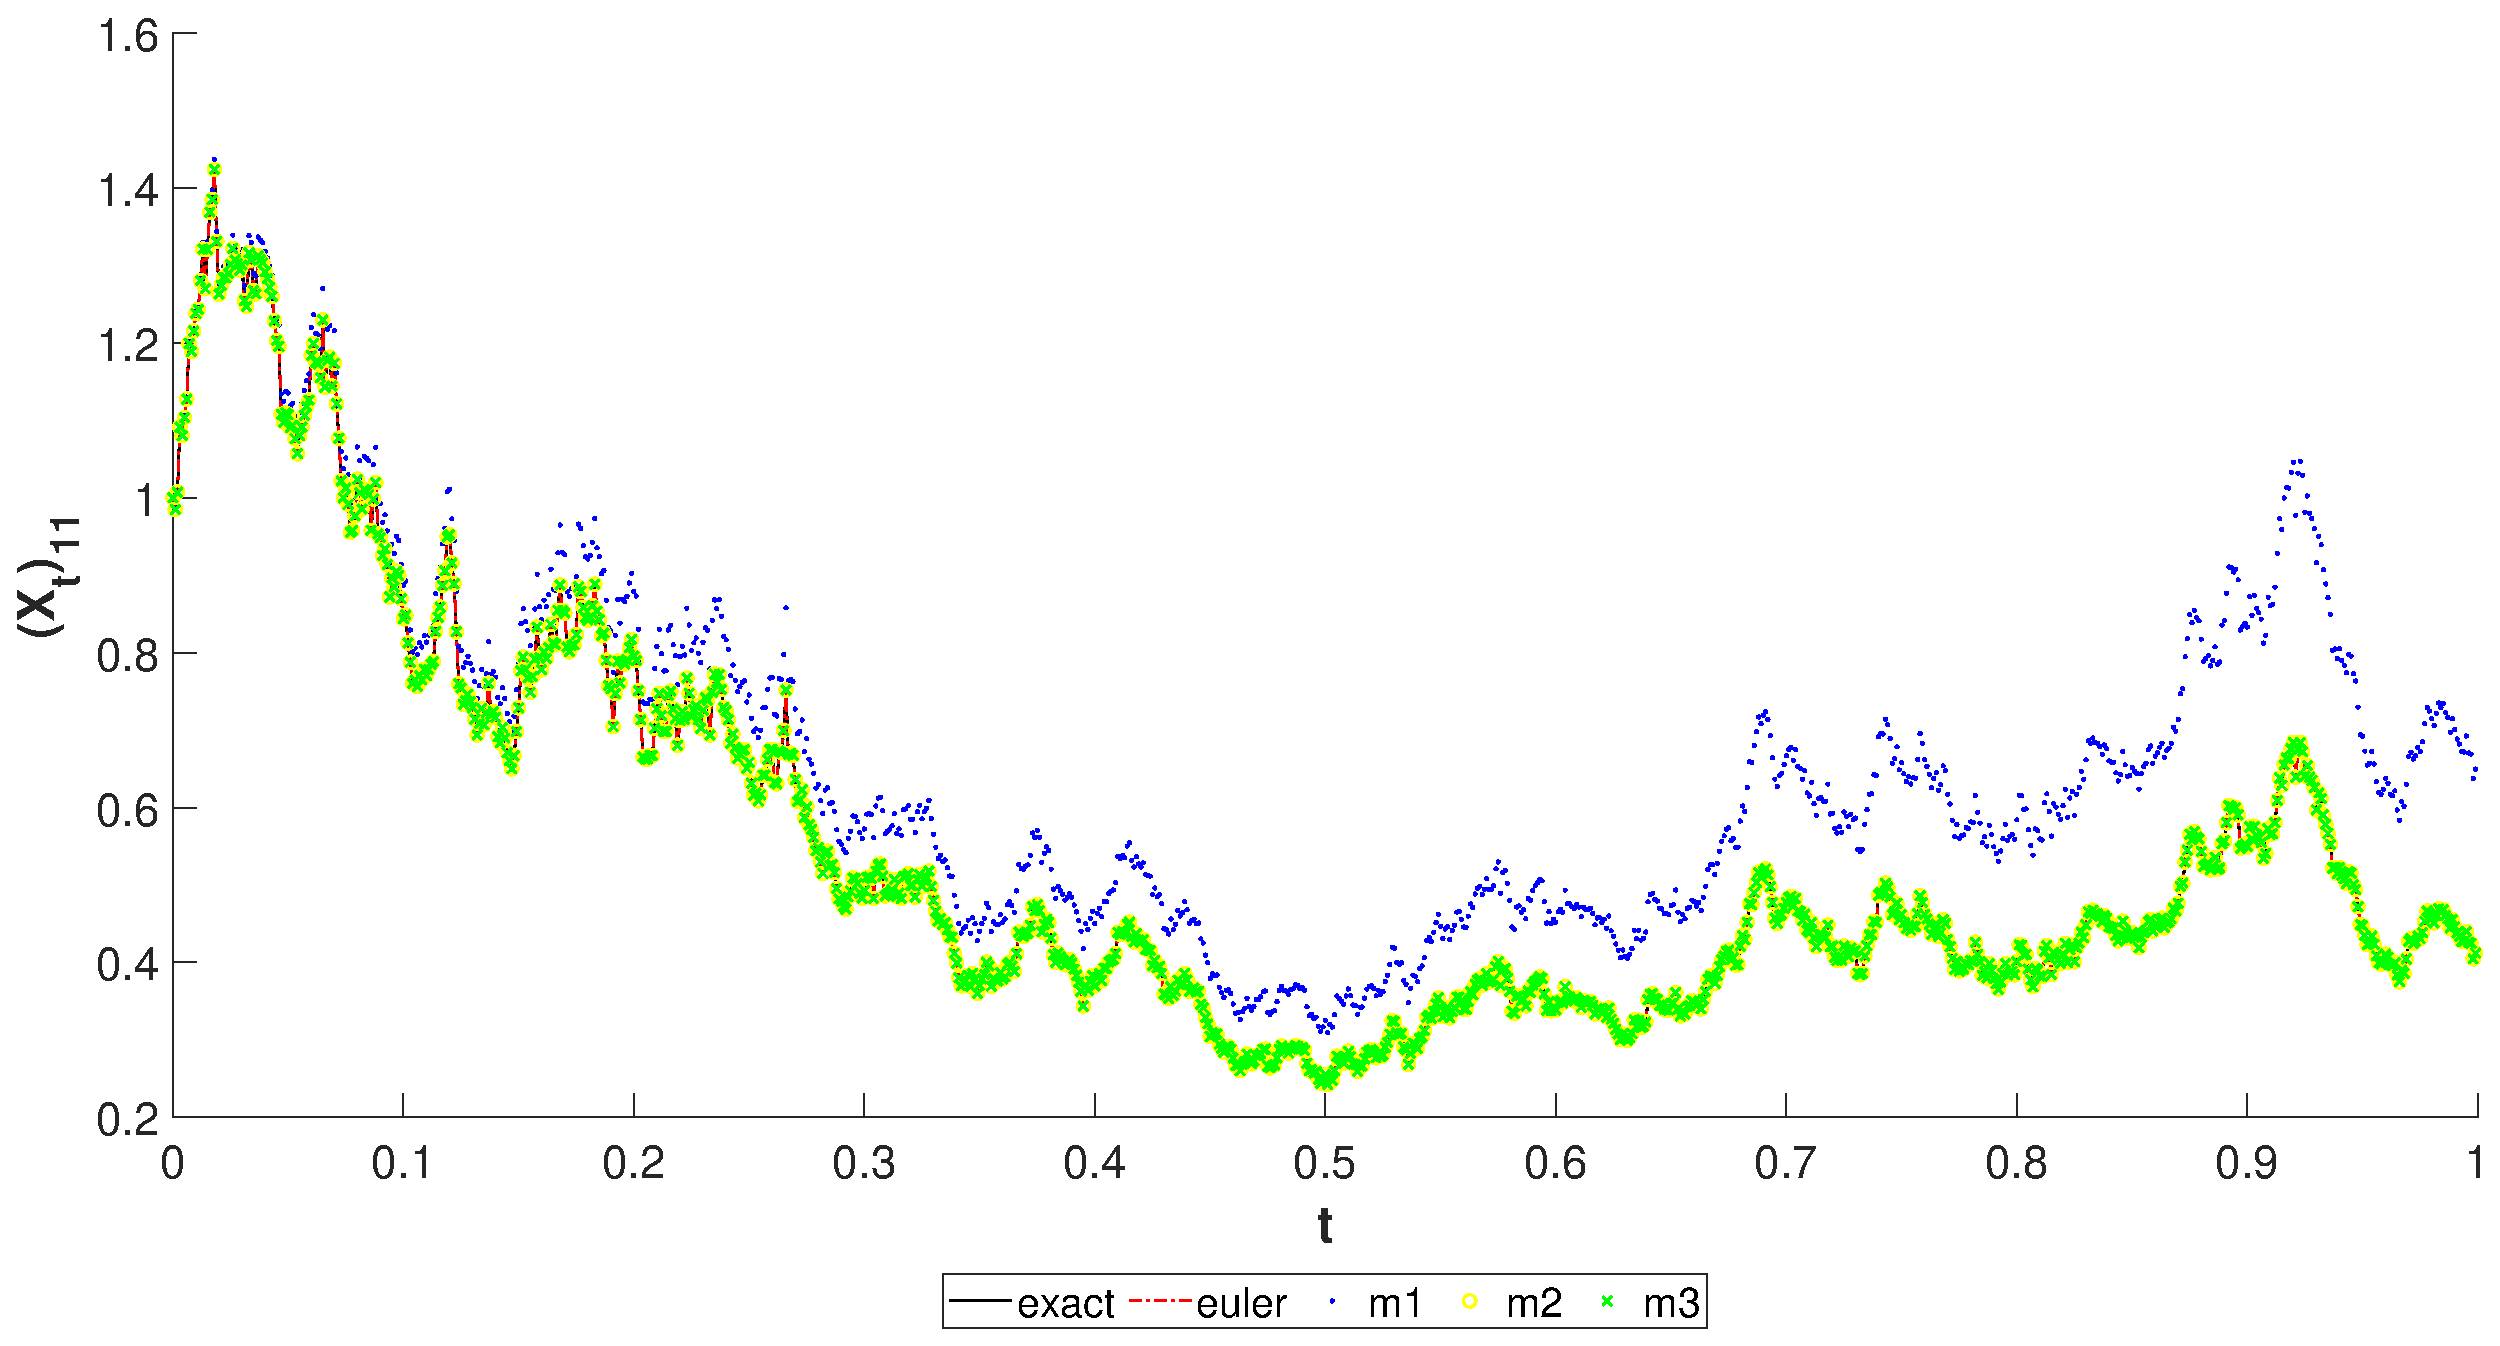
\includegraphics[width=.95\columnwidth]{C:/Users/kevin/Documents/MATLAB/PhD/Magnus/Final/Correction/B0_var/Pdf/temp/plot_1.eps}
\end{landscape}
\begin{landscape}
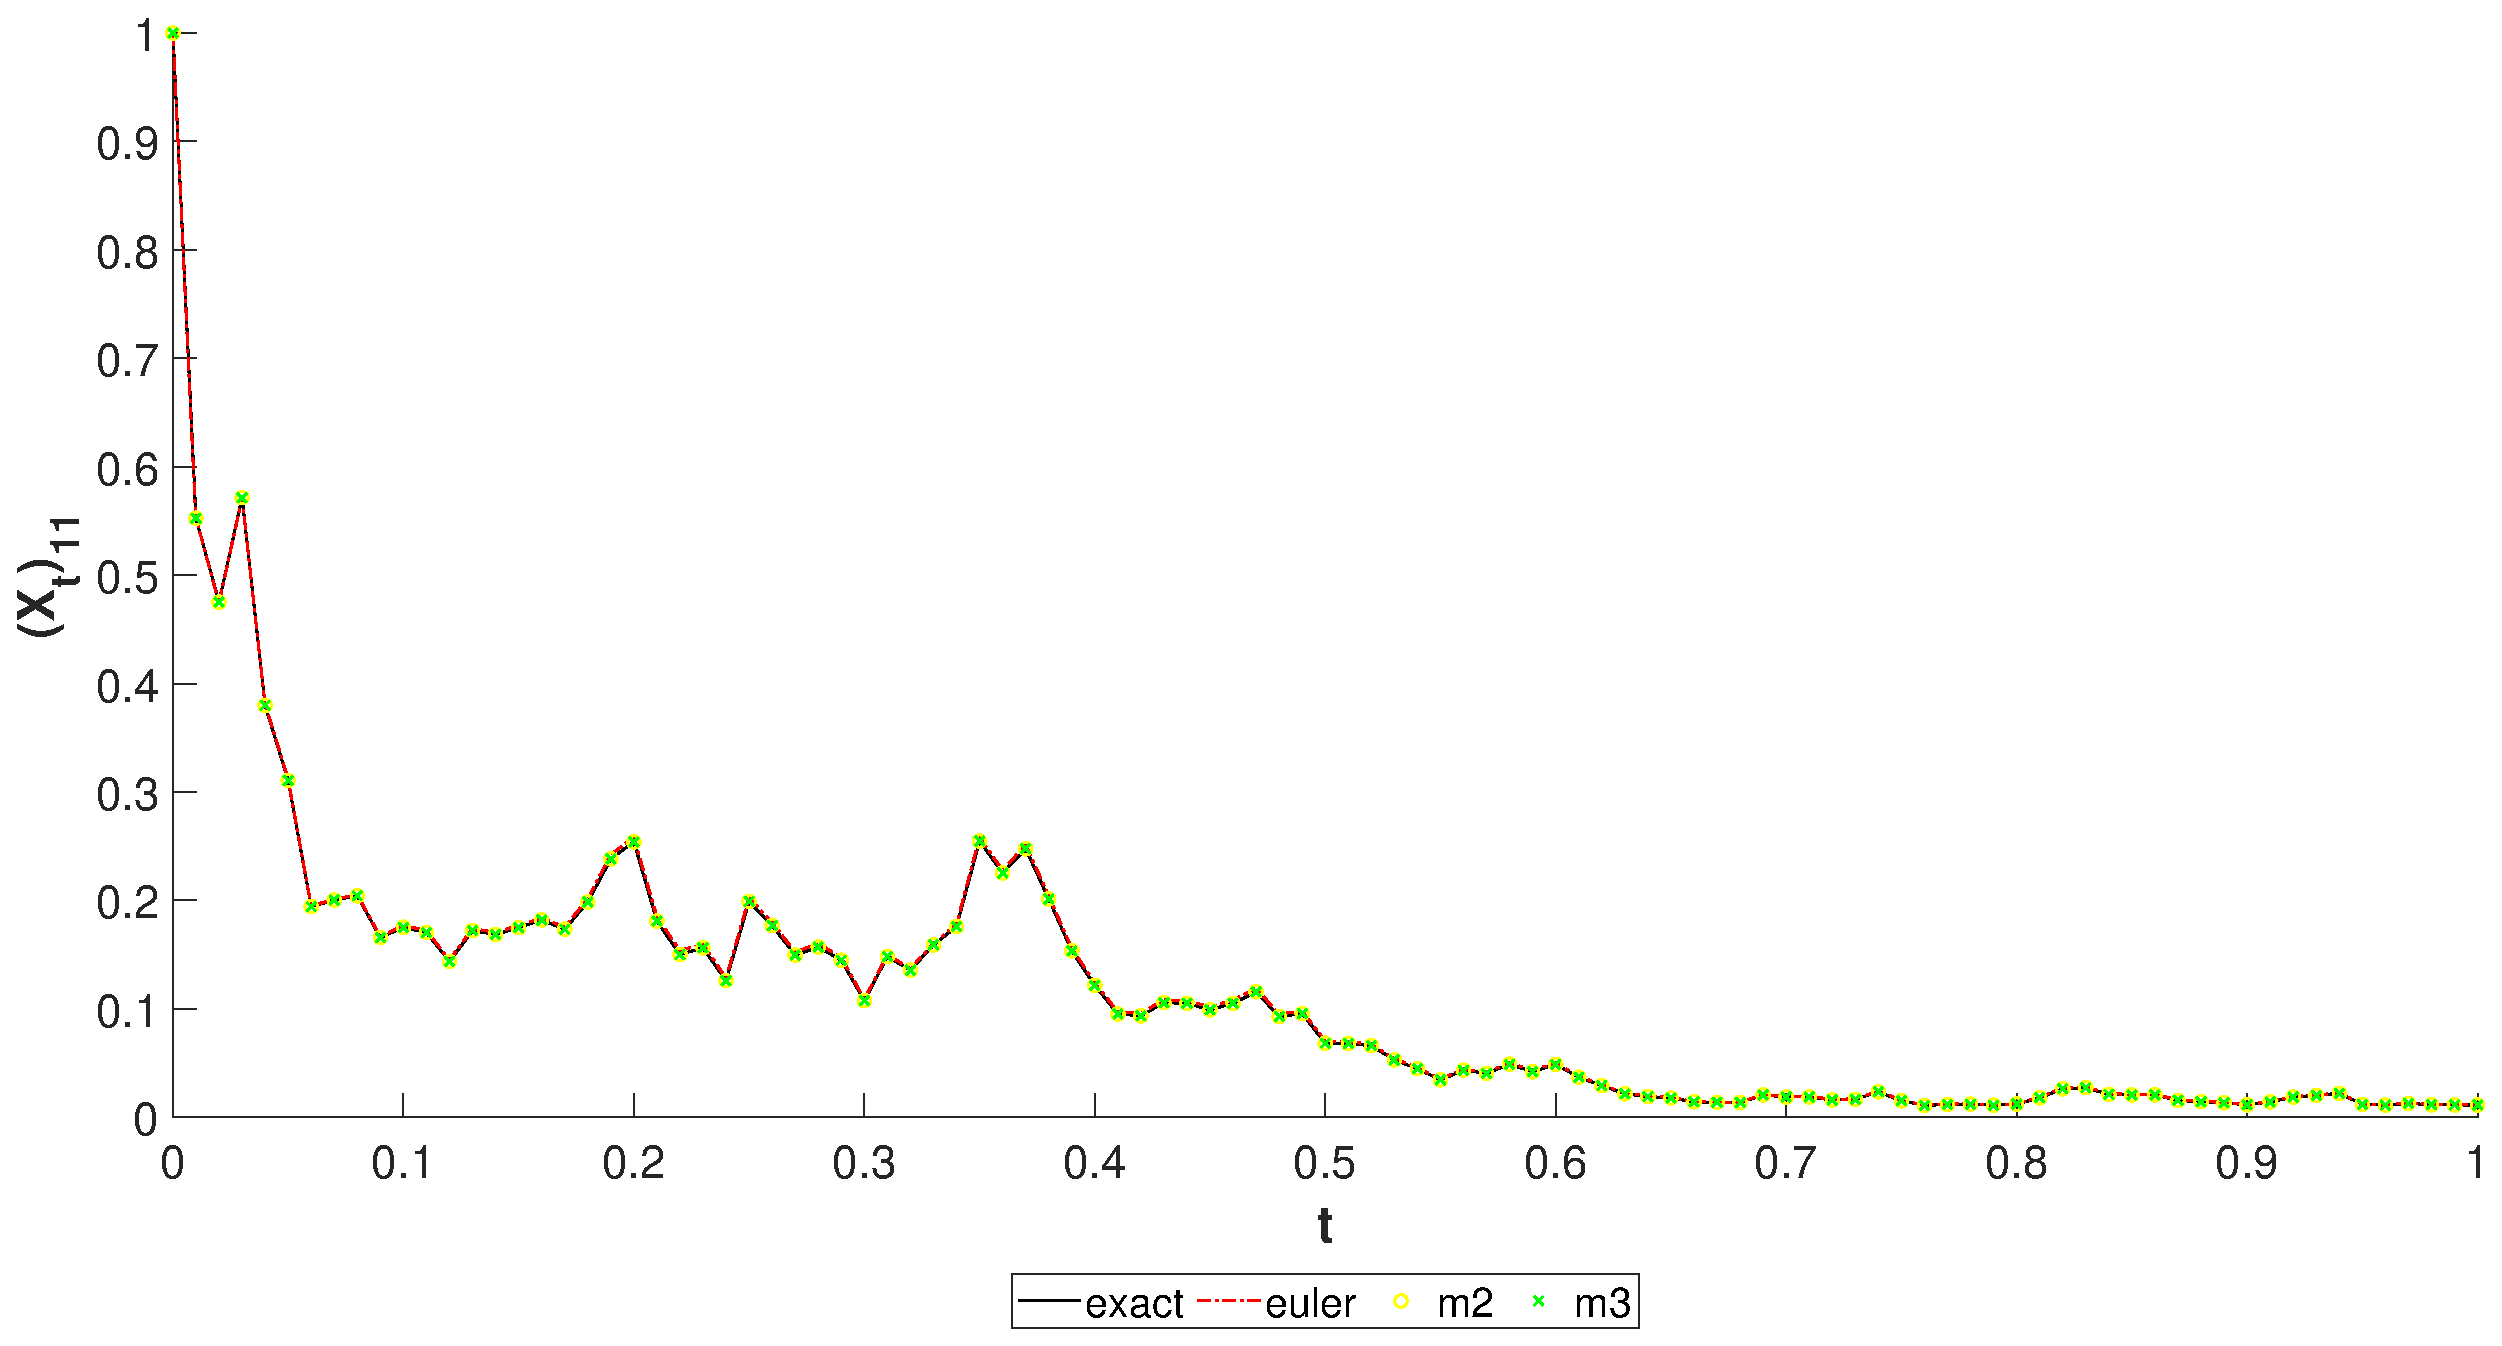
\includegraphics[width=.95\columnwidth]{C:/Users/kevin/Documents/MATLAB/PhD/Magnus/Final/Correction/B0_var/Pdf/temp/plot_2.eps}
\end{landscape}
\begin{landscape}
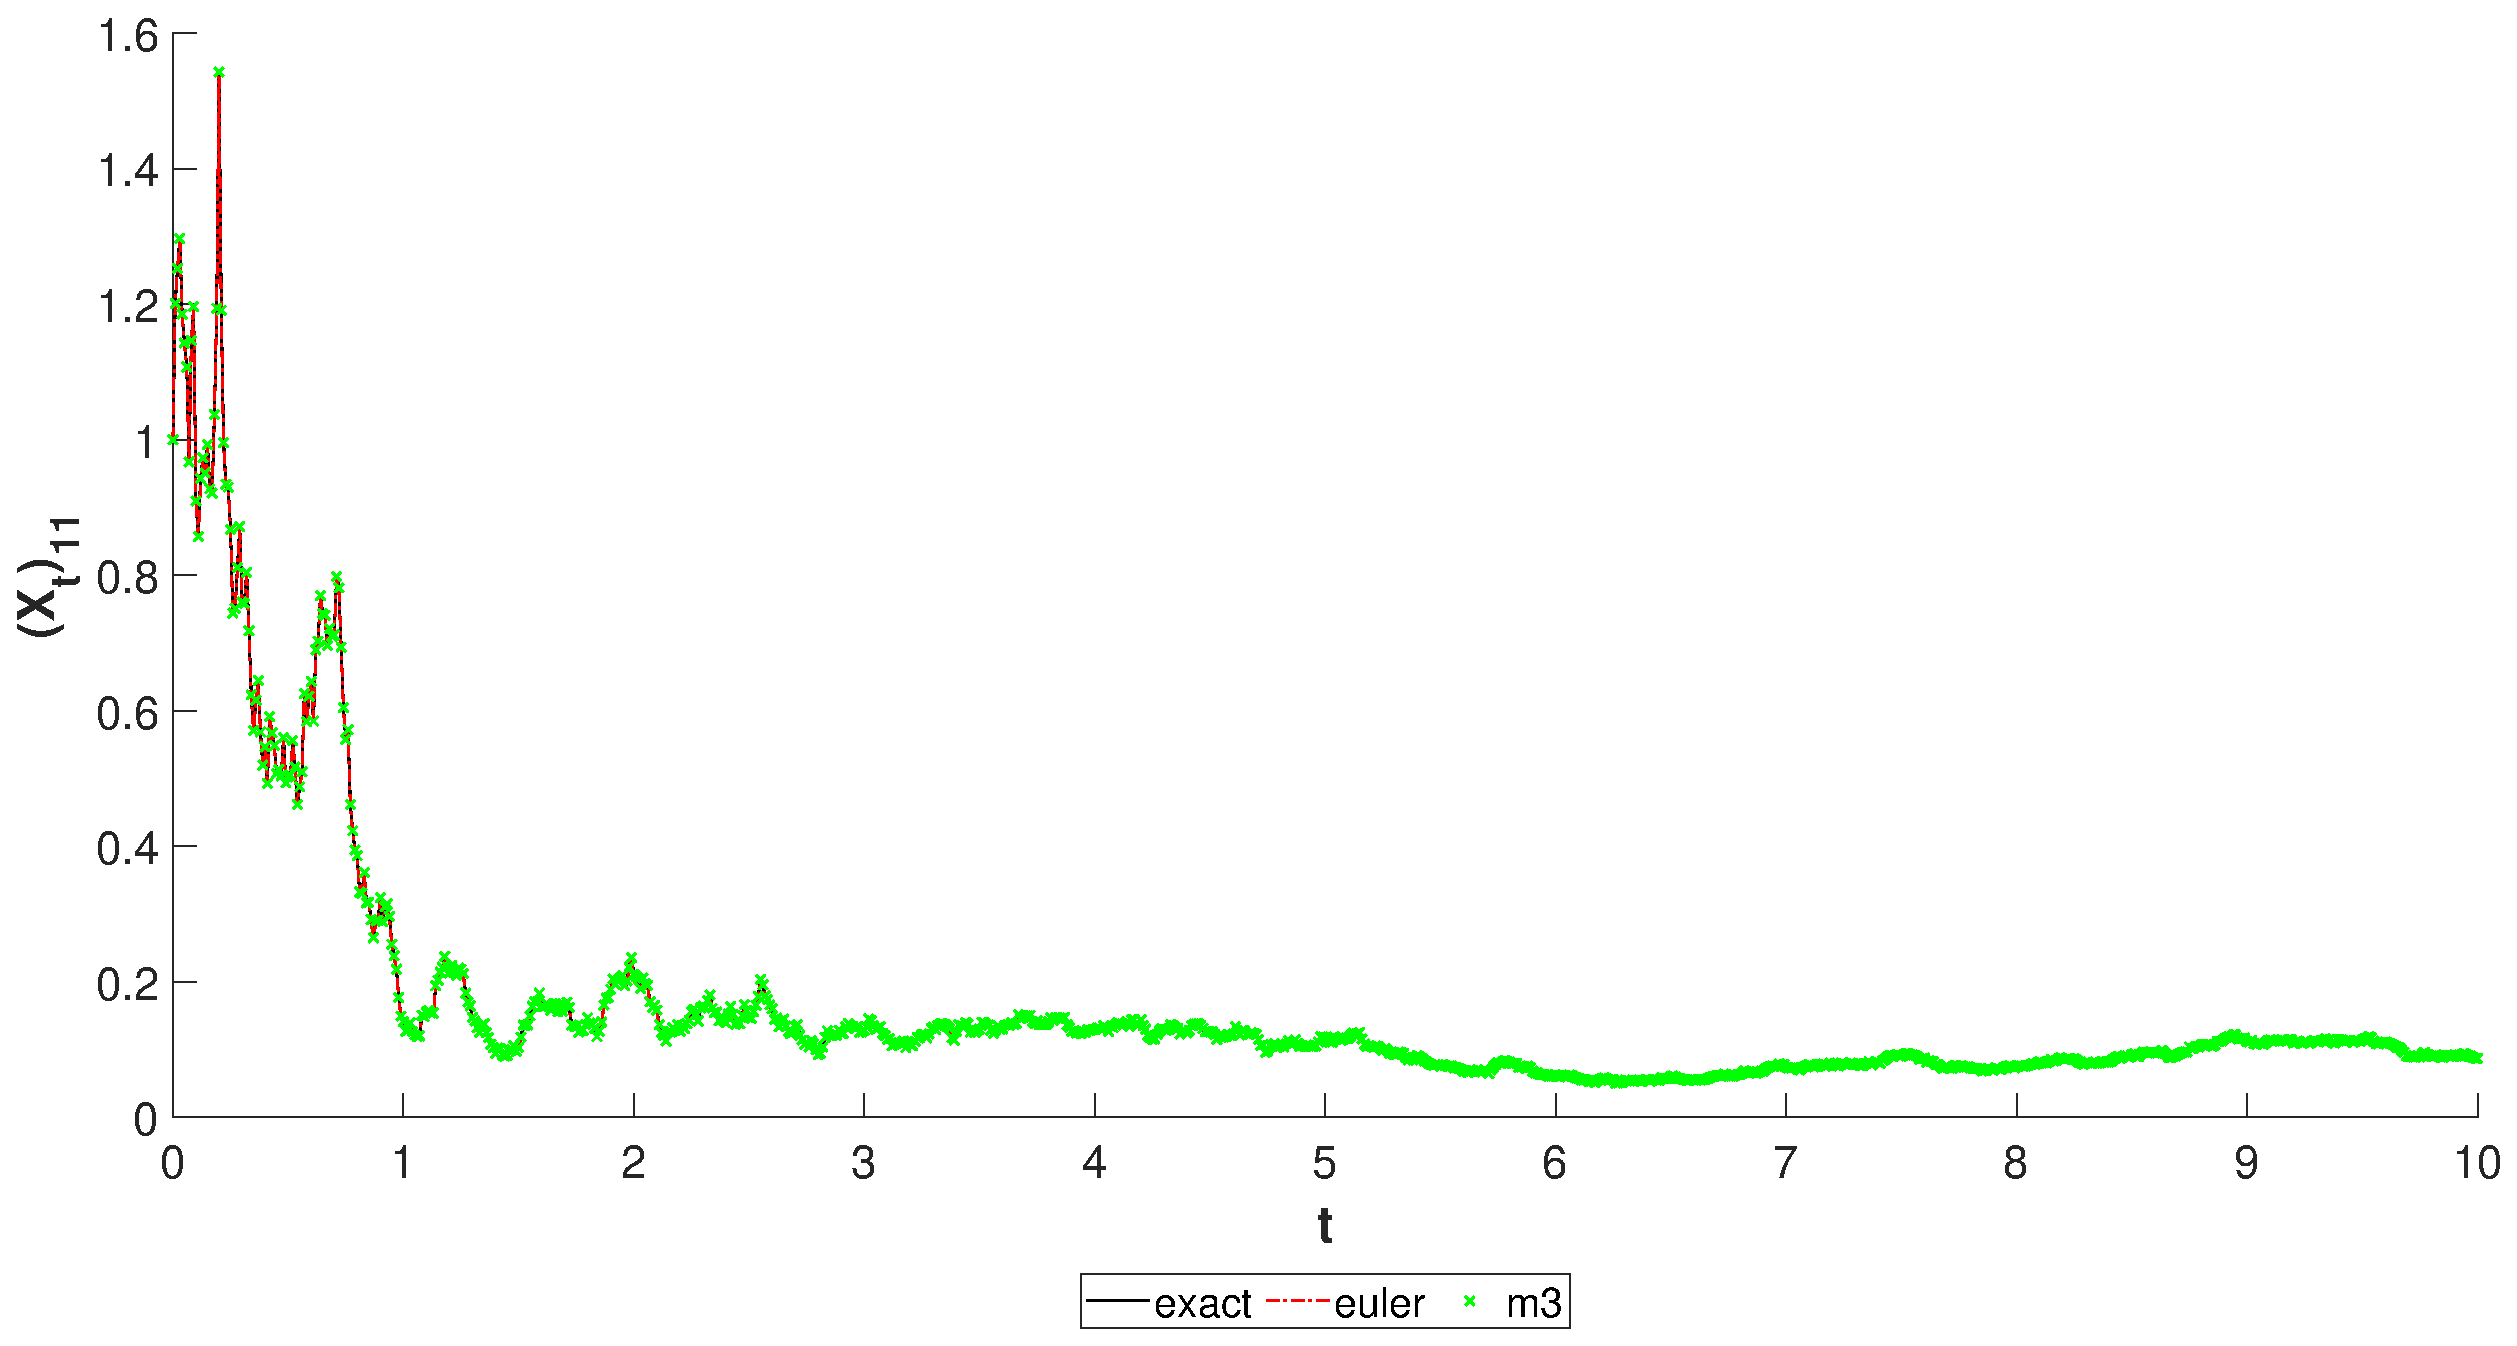
\includegraphics[width=.95\columnwidth]{C:/Users/kevin/Documents/MATLAB/PhD/Magnus/Final/Correction/B0_var/Pdf/temp/plot_3.eps}
\end{landscape}
\begin{landscape}
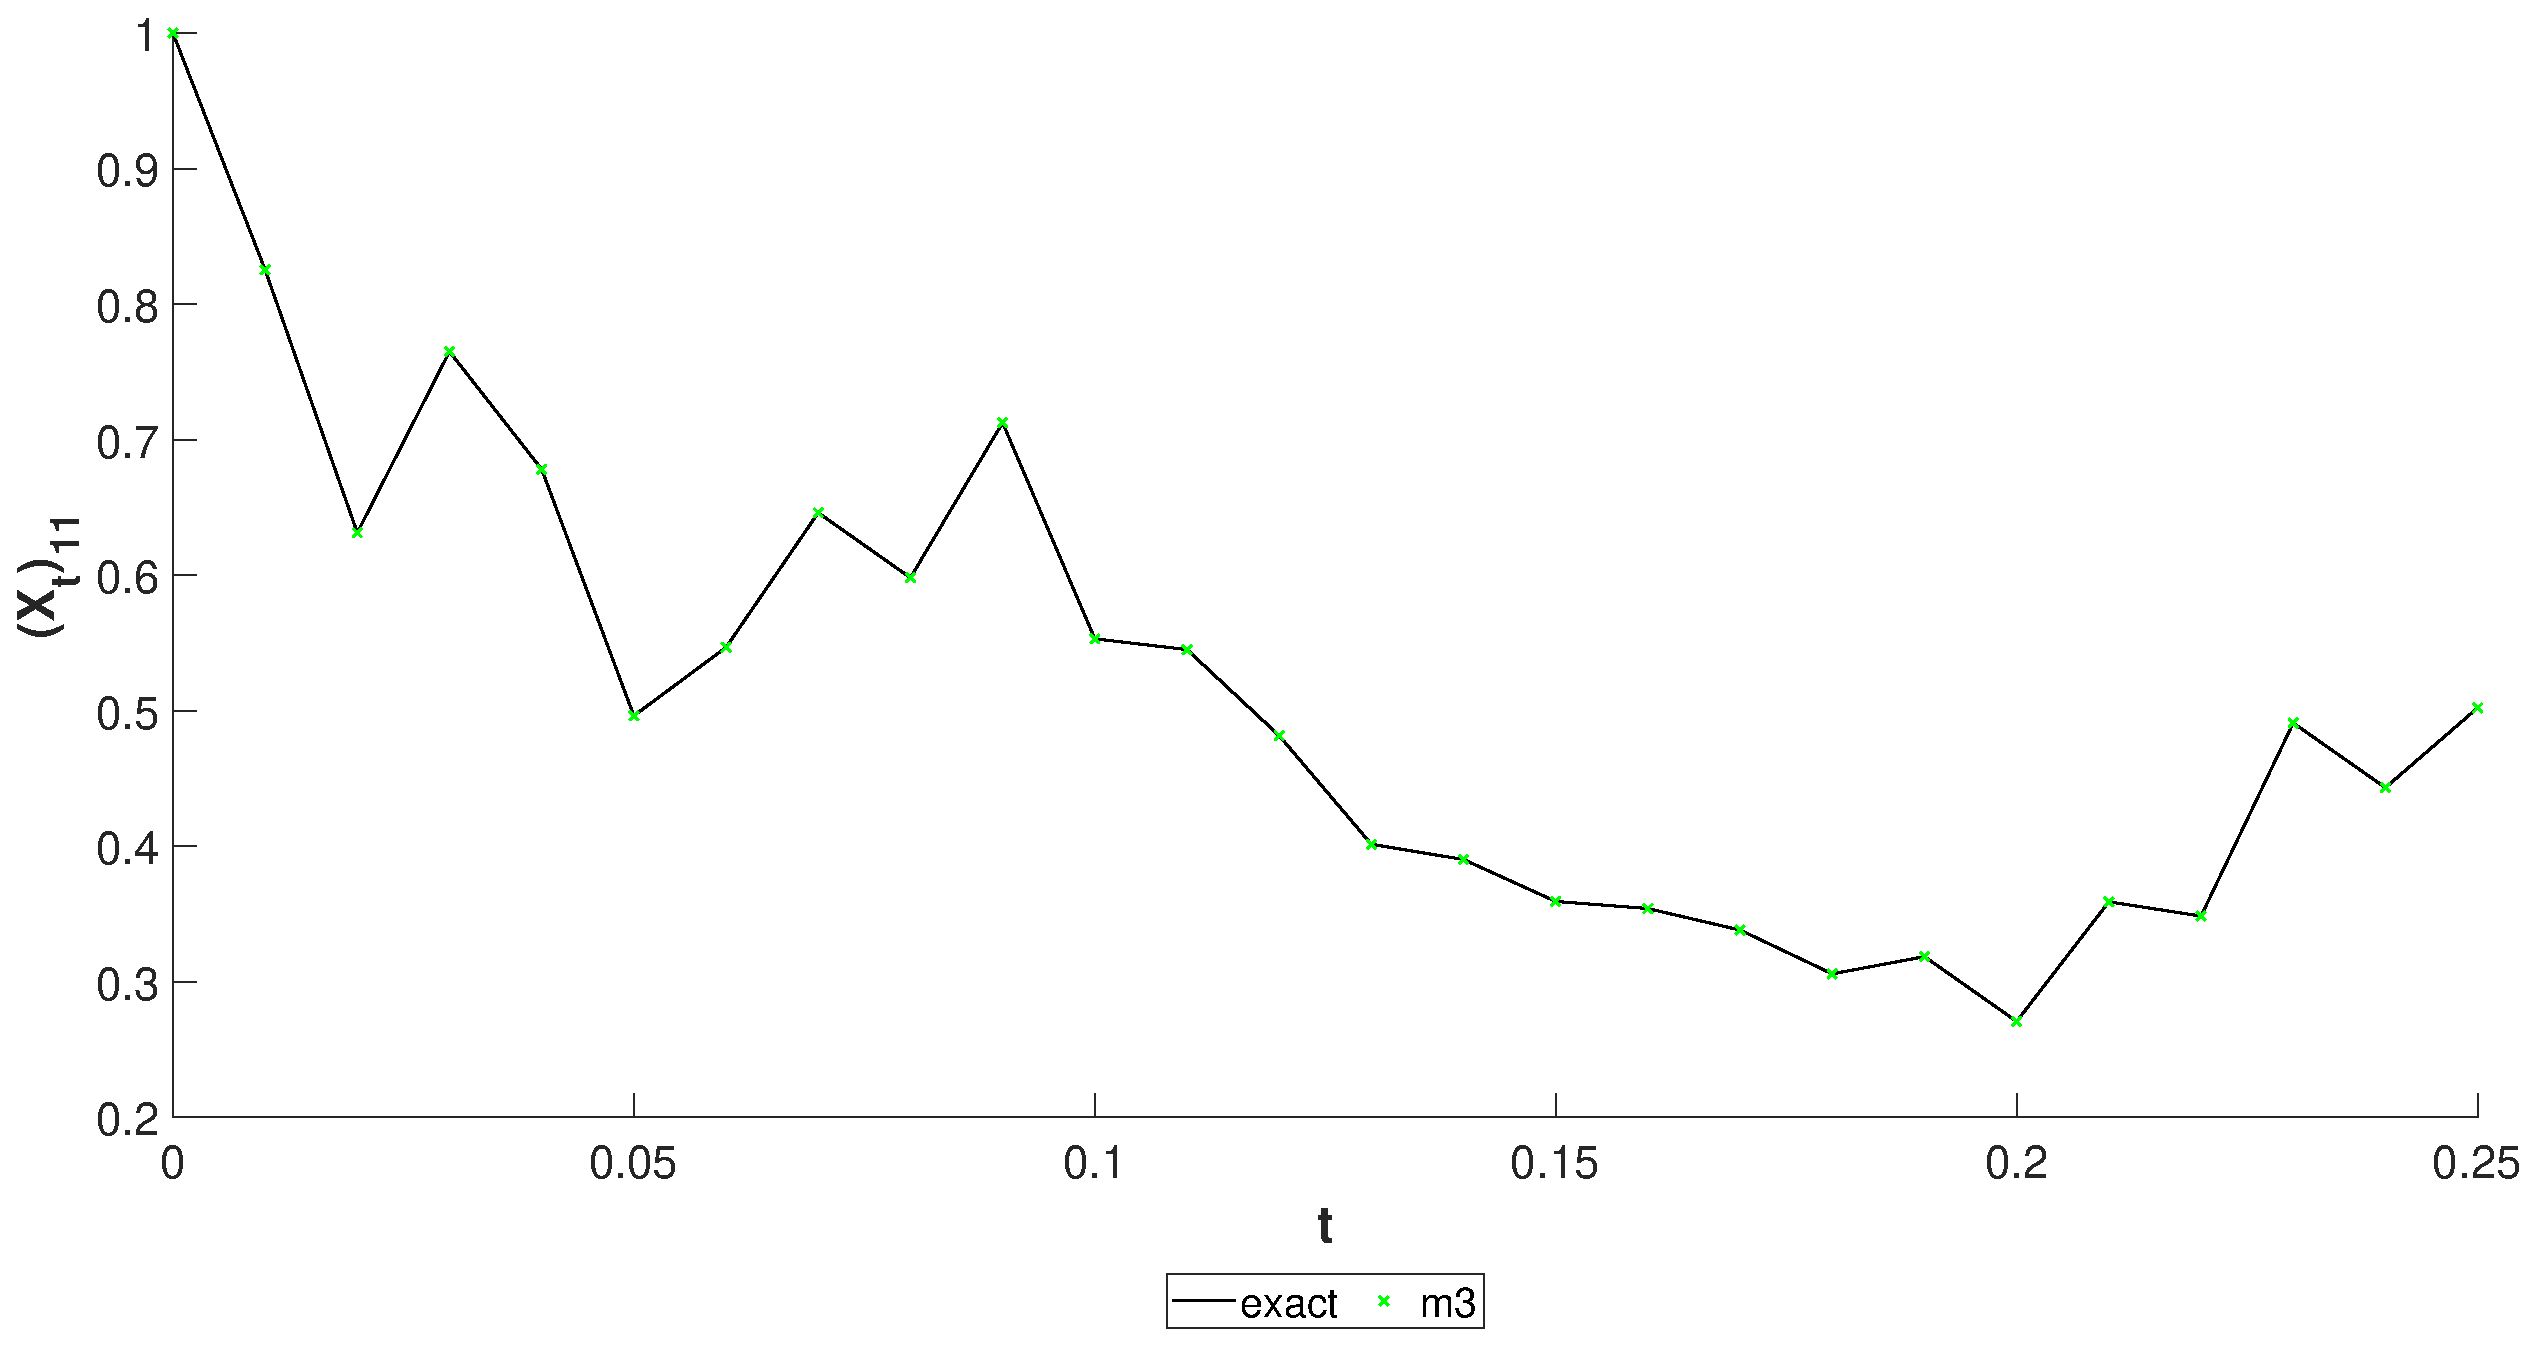
\includegraphics[width=.95\columnwidth]{C:/Users/kevin/Documents/MATLAB/PhD/Magnus/Final/Correction/B0_var/Pdf/temp/plot_4.eps}
\end{landscape}
\begin{landscape}
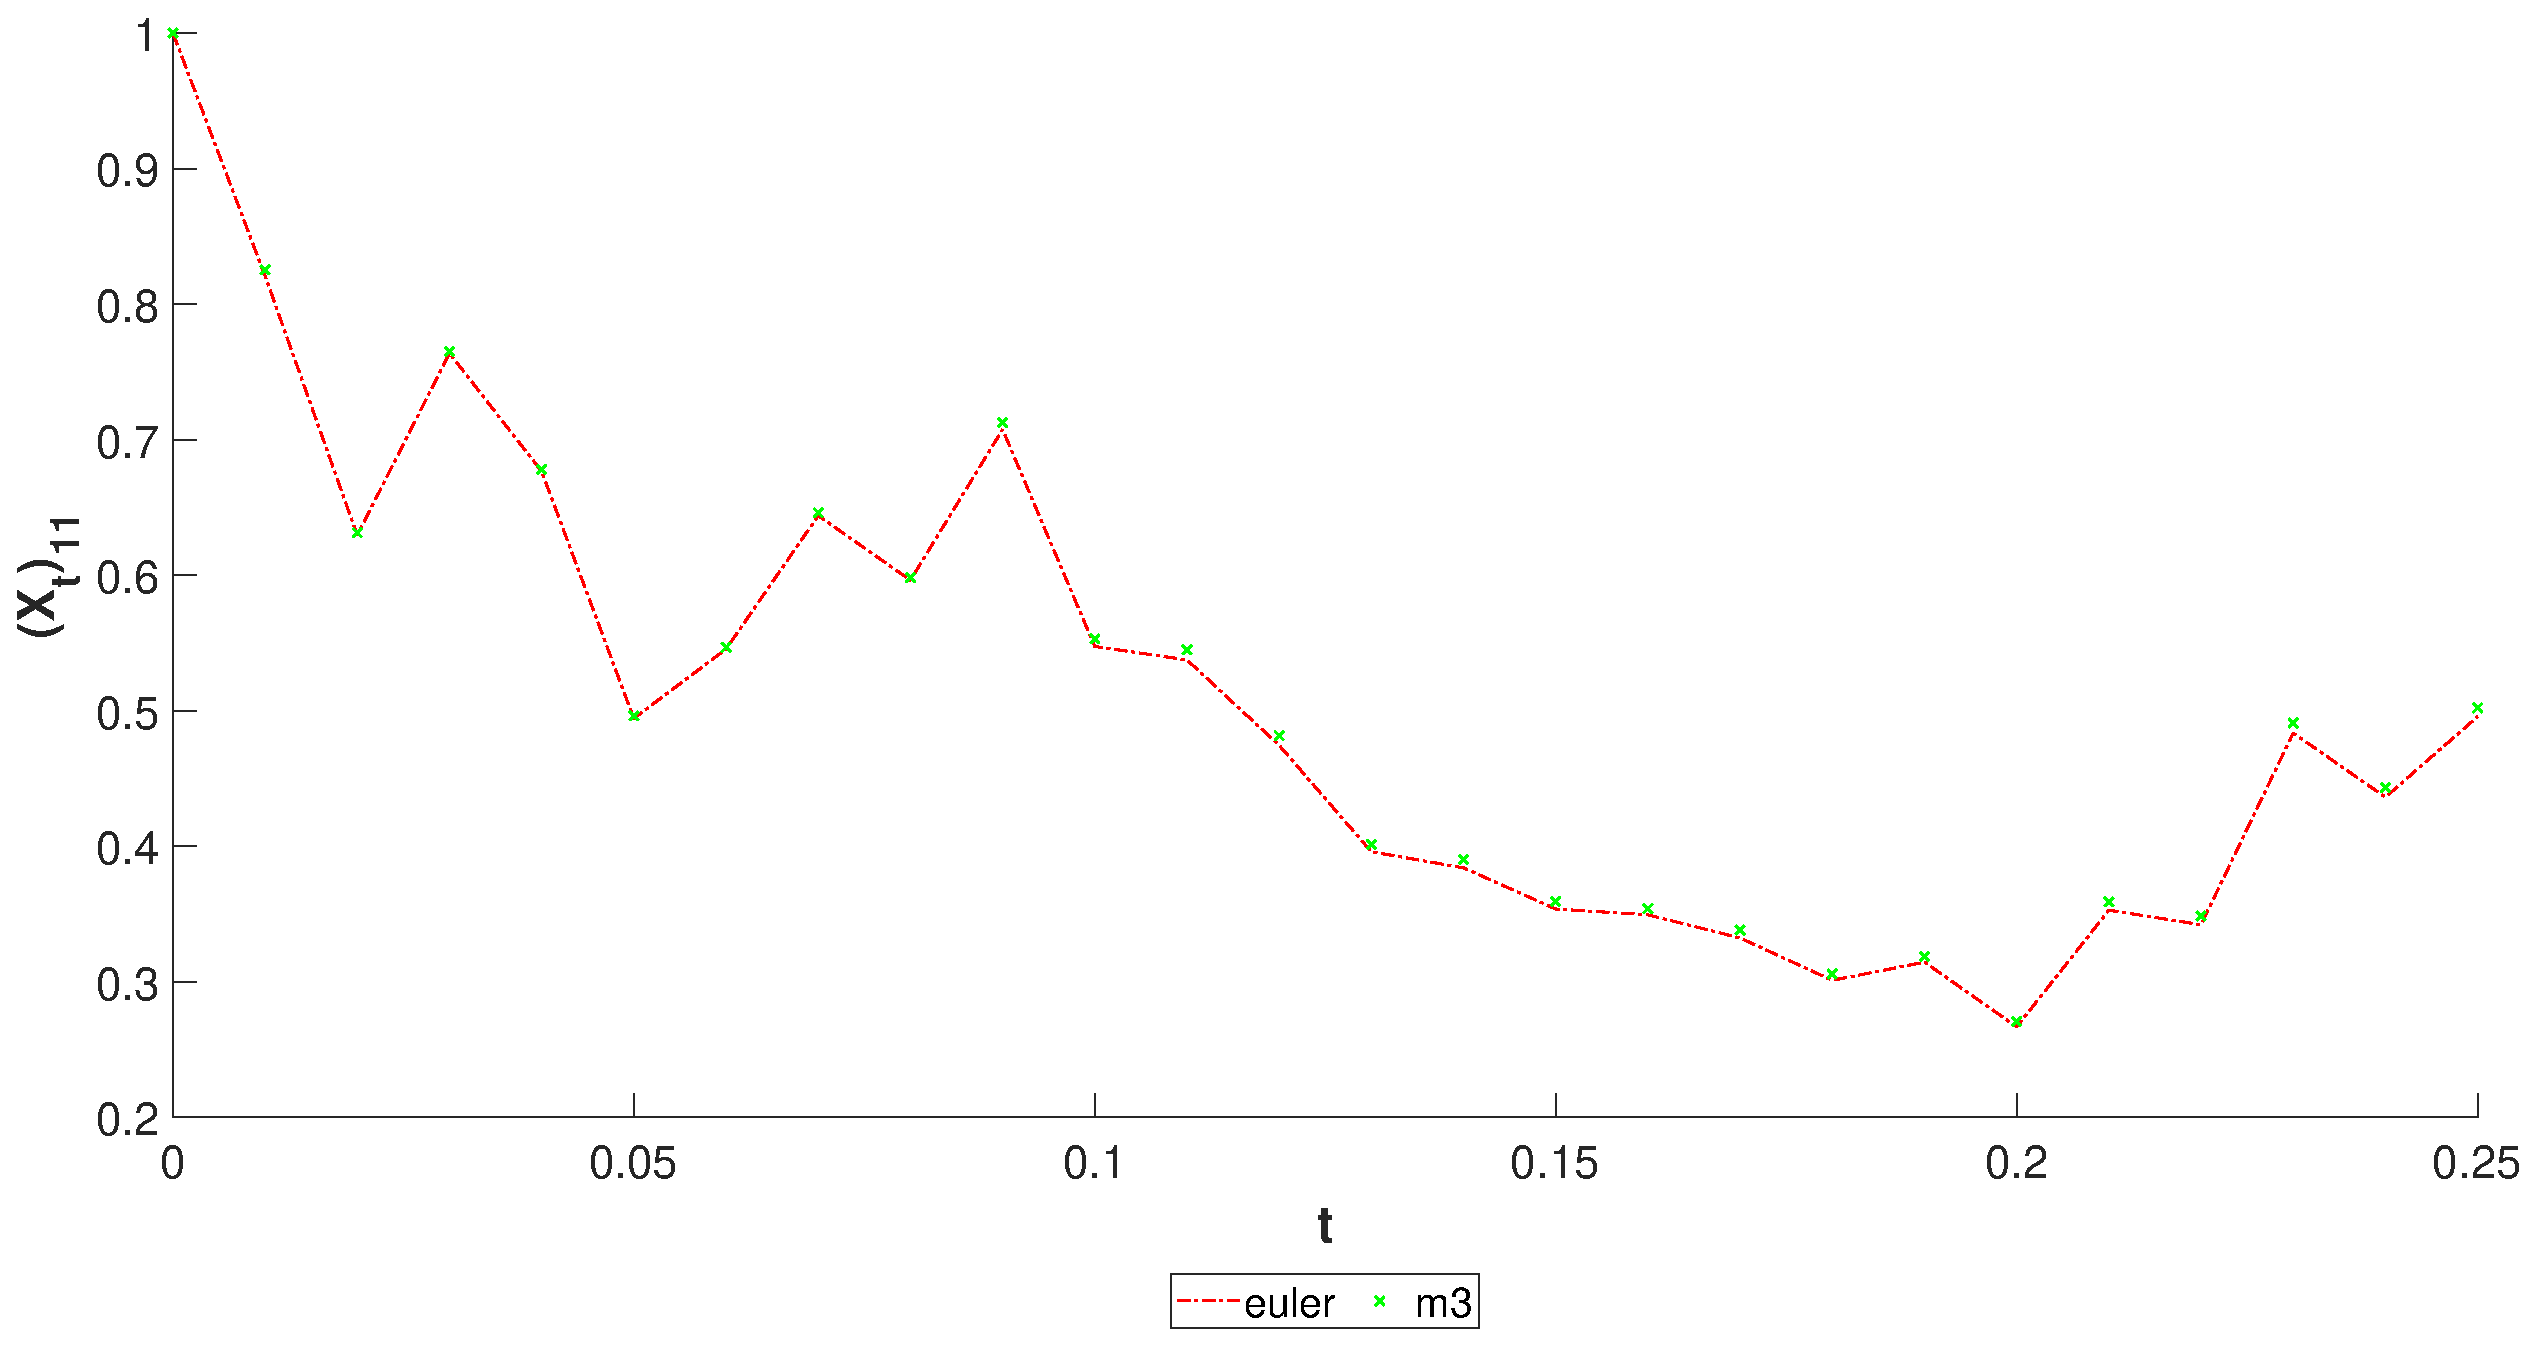
\includegraphics[width=.95\columnwidth]{C:/Users/kevin/Documents/MATLAB/PhD/Magnus/Final/Correction/B0_var/Pdf/temp/plot_5.eps}
\end{landscape}
\begin{landscape}
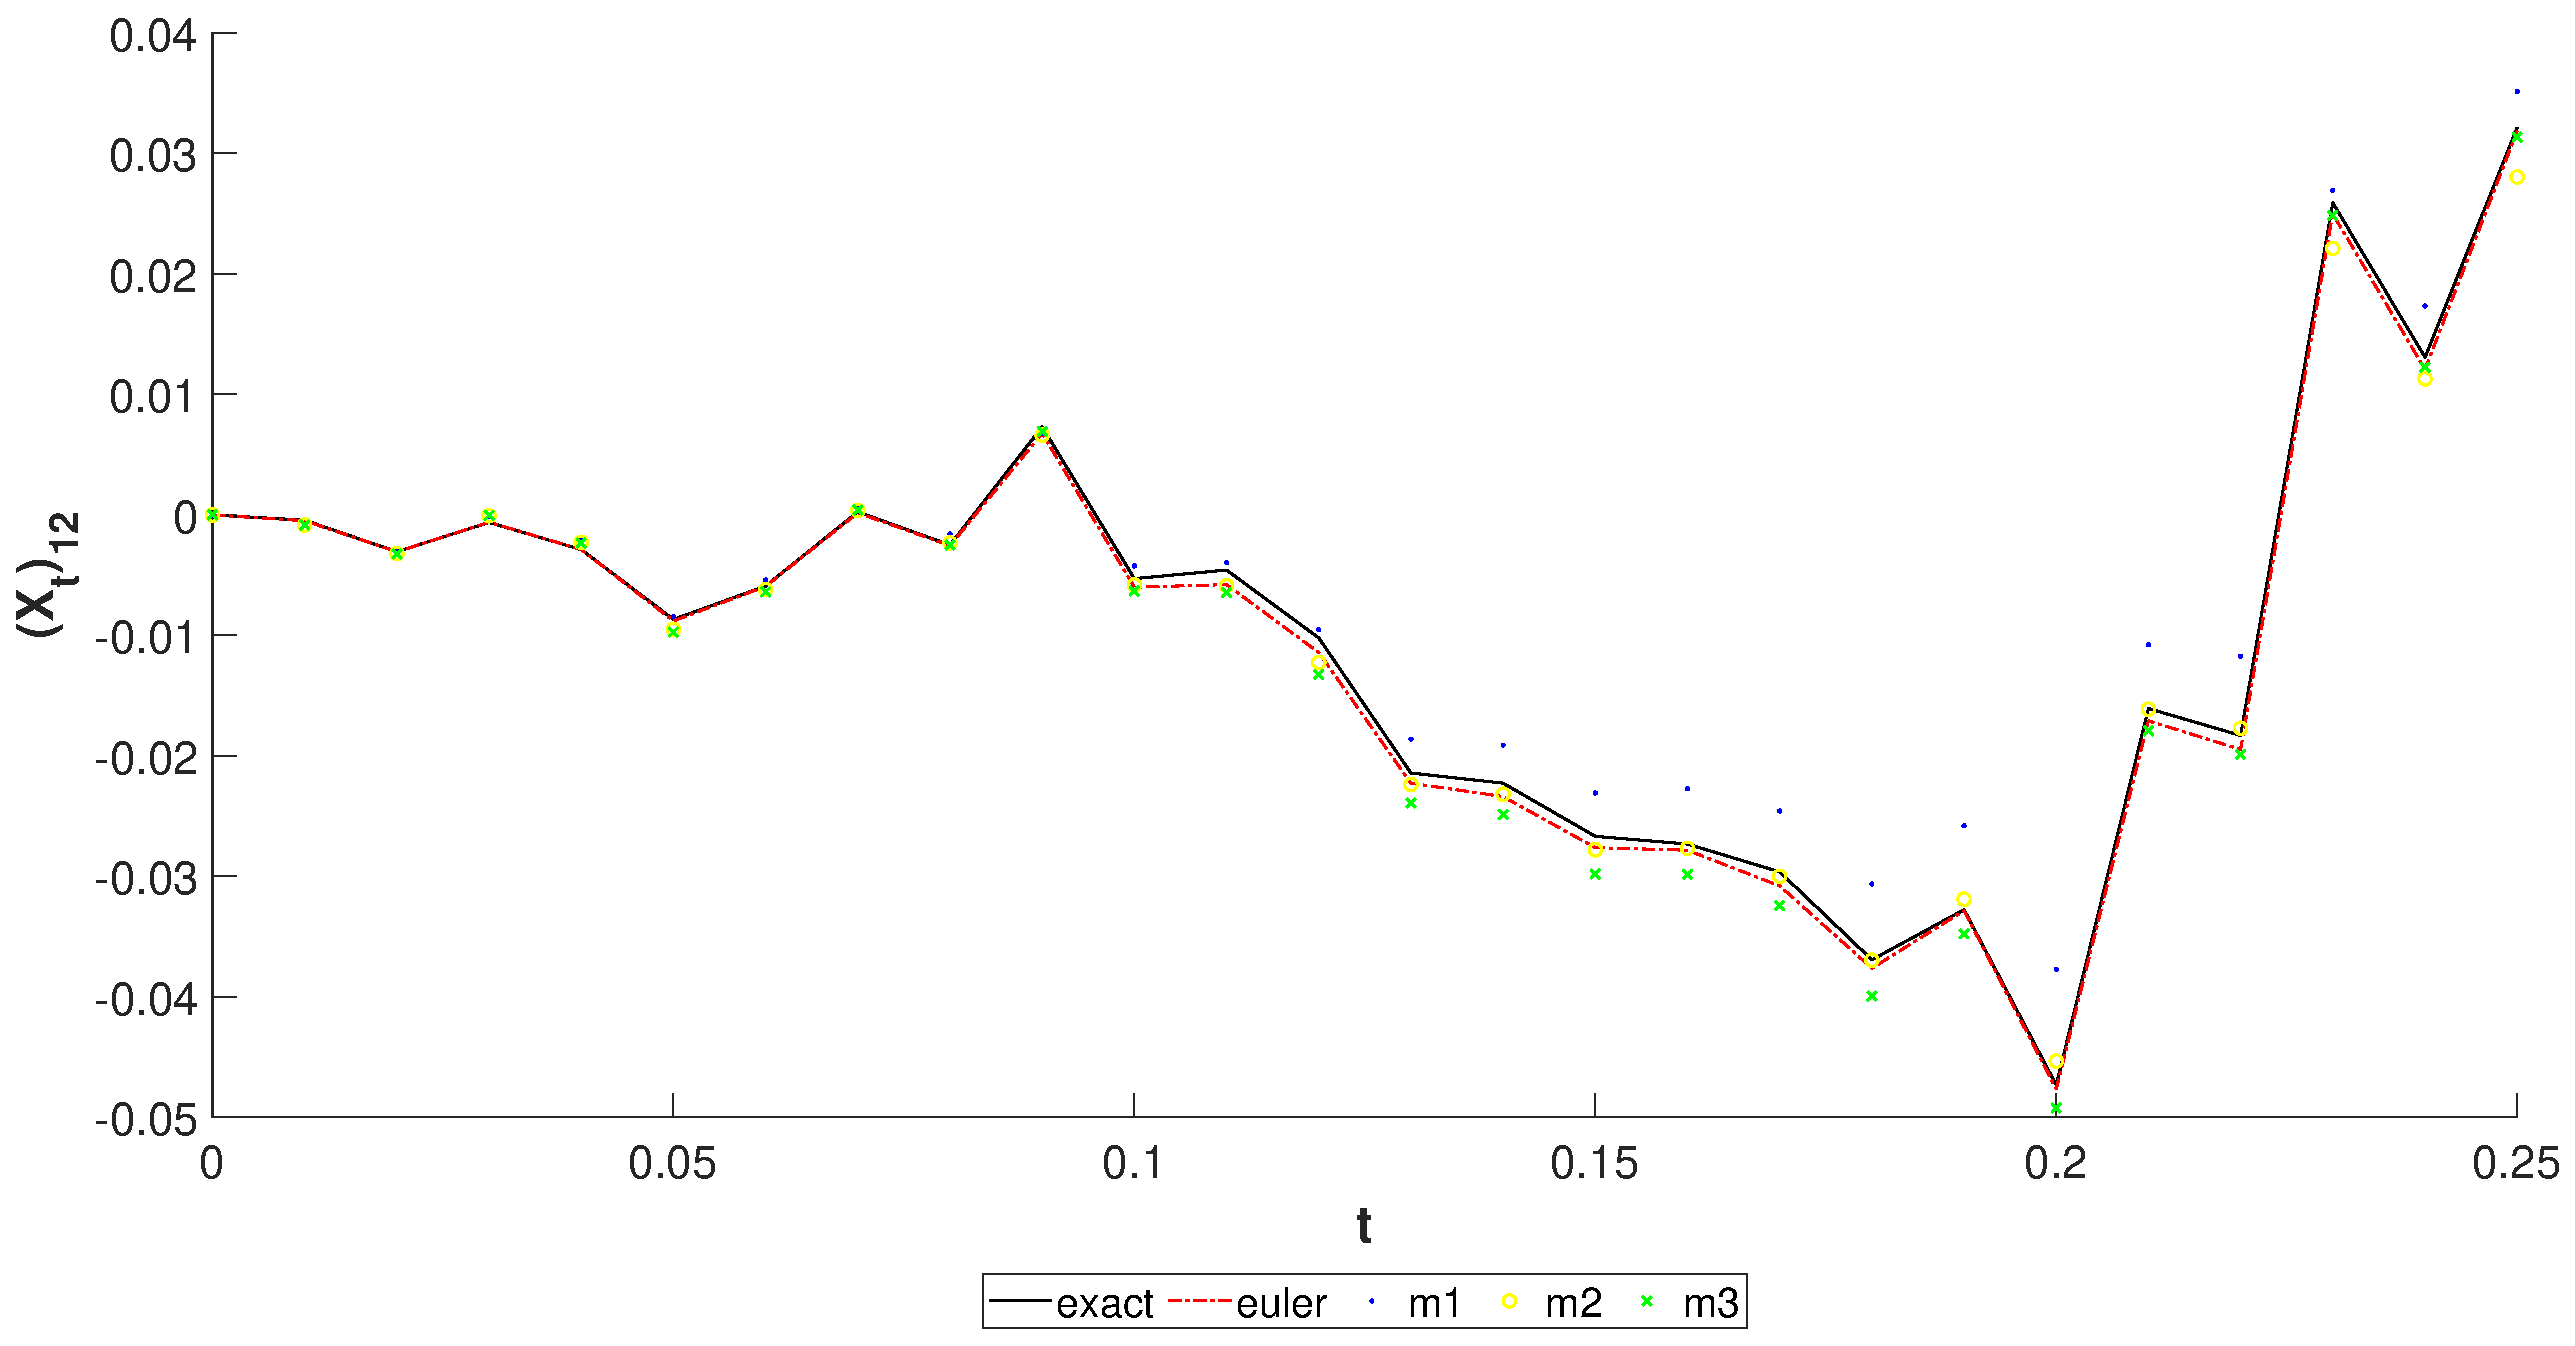
\includegraphics[width=.95\columnwidth]{C:/Users/kevin/Documents/MATLAB/PhD/Magnus/Final/Correction/B0_var/Pdf/temp/plot_6.eps}
\end{landscape}
\begin{landscape}
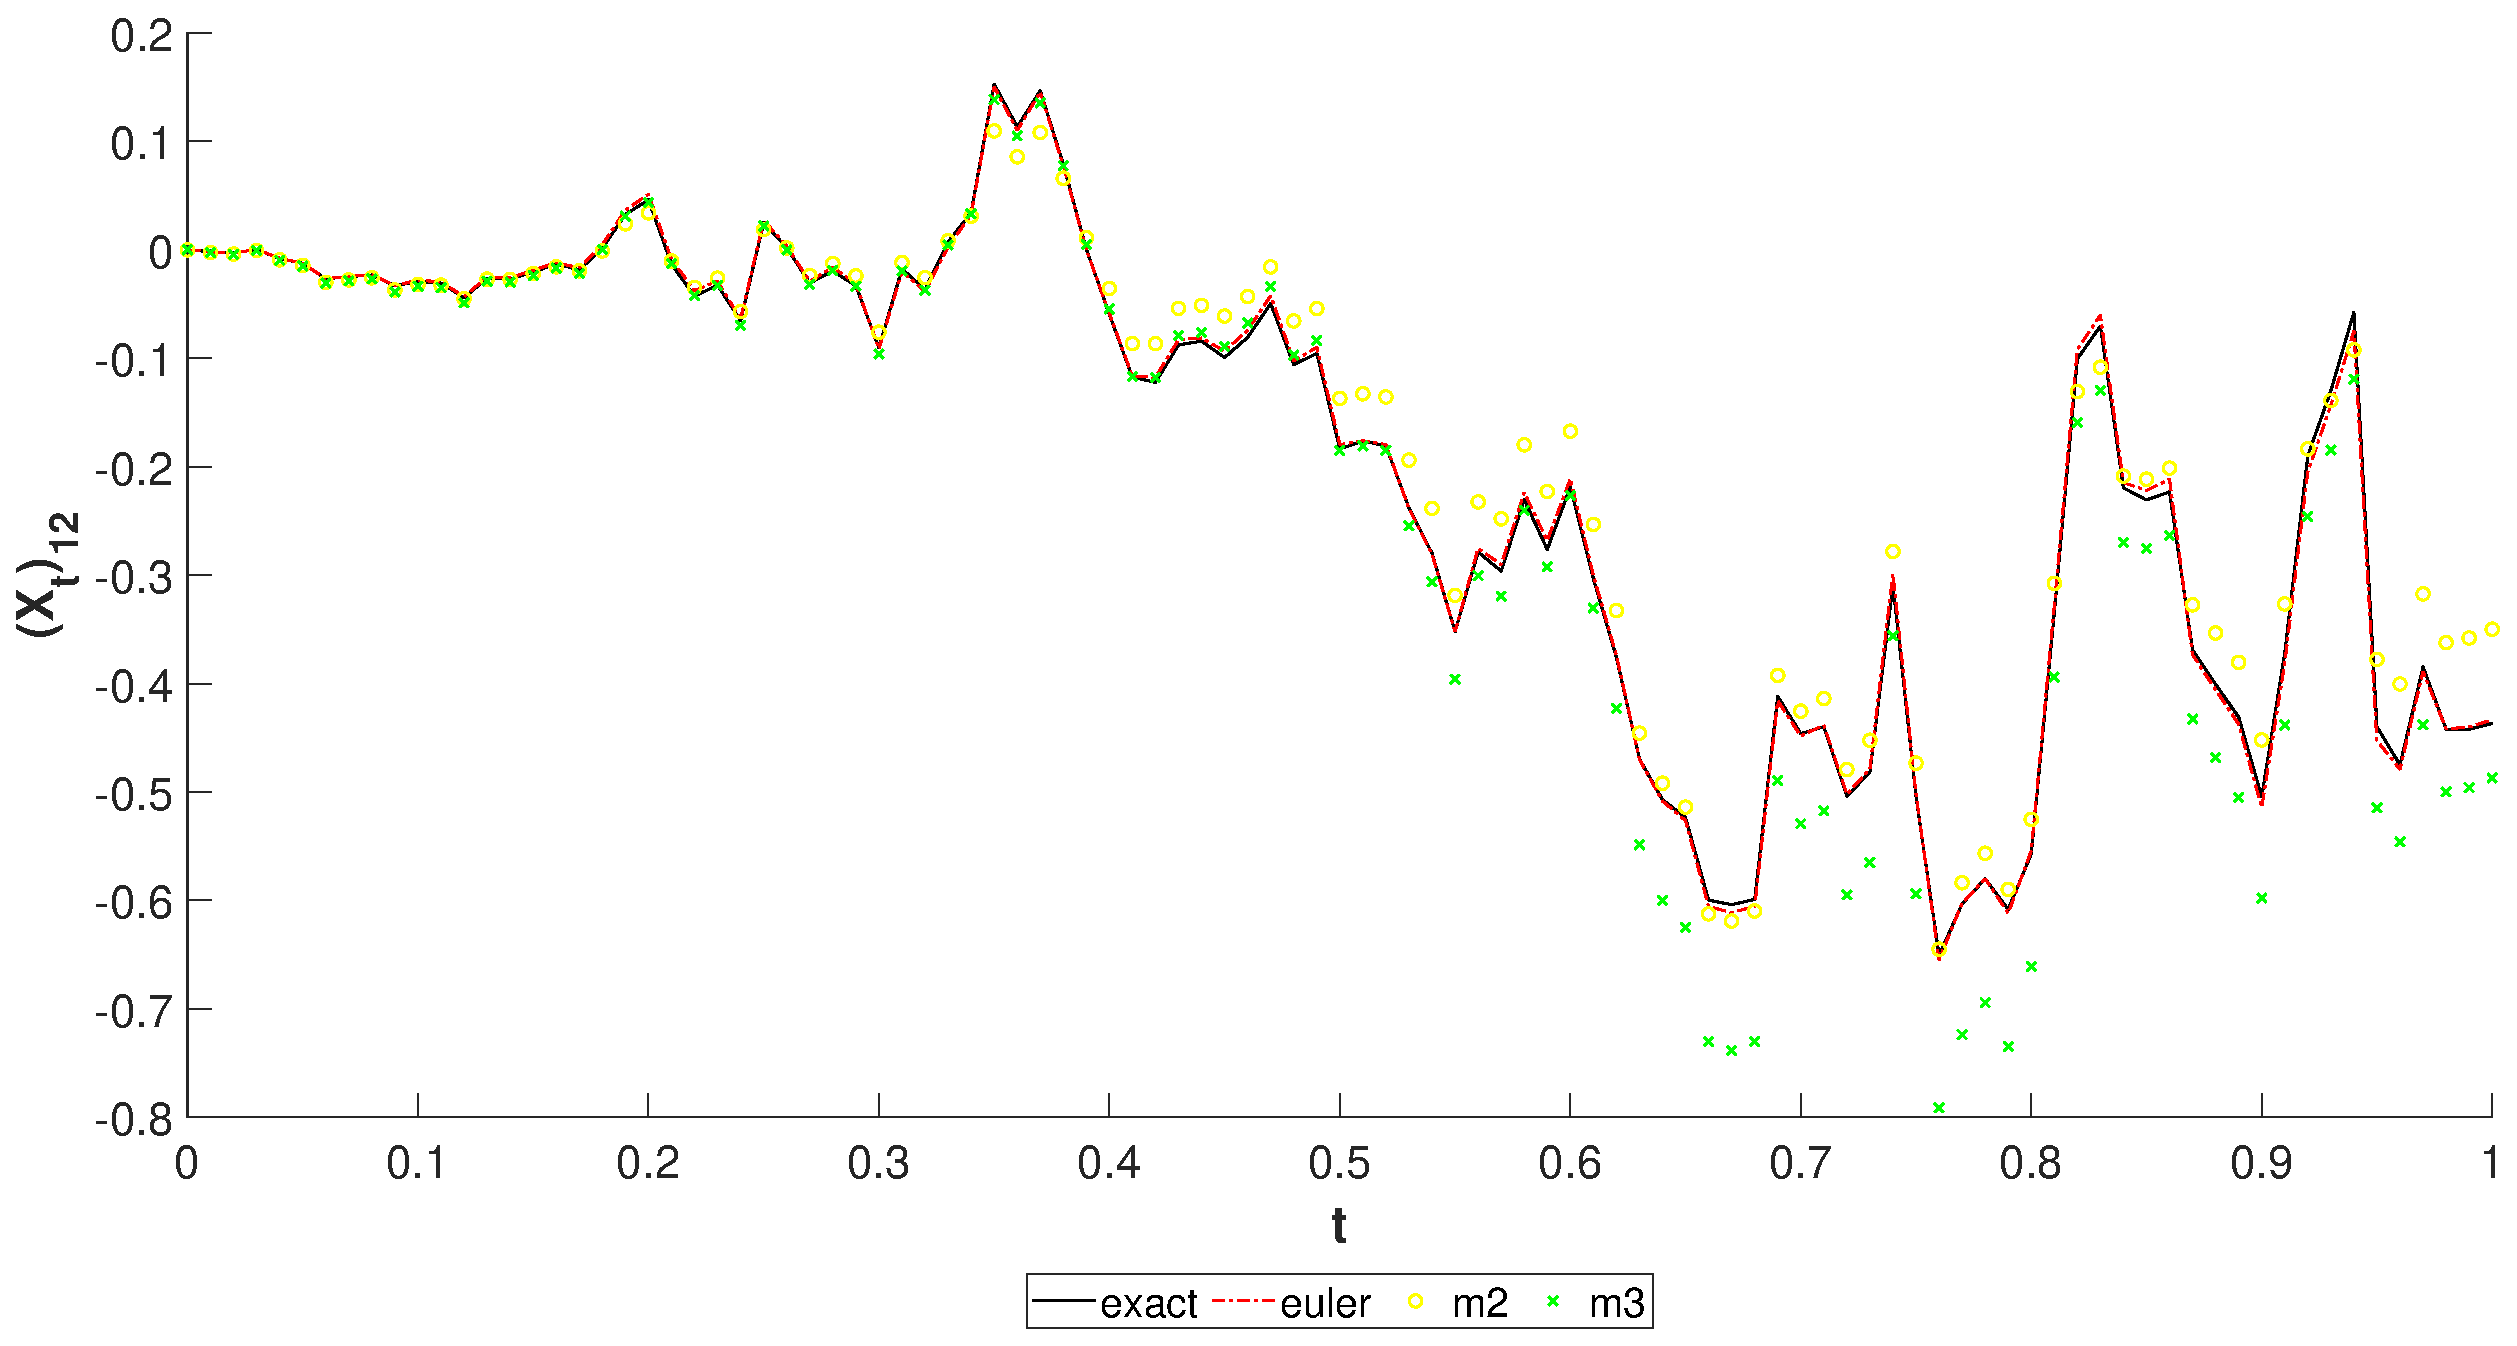
\includegraphics[width=.95\columnwidth]{C:/Users/kevin/Documents/MATLAB/PhD/Magnus/Final/Correction/B0_var/Pdf/temp/plot_7.eps}
\end{landscape}
\begin{landscape}
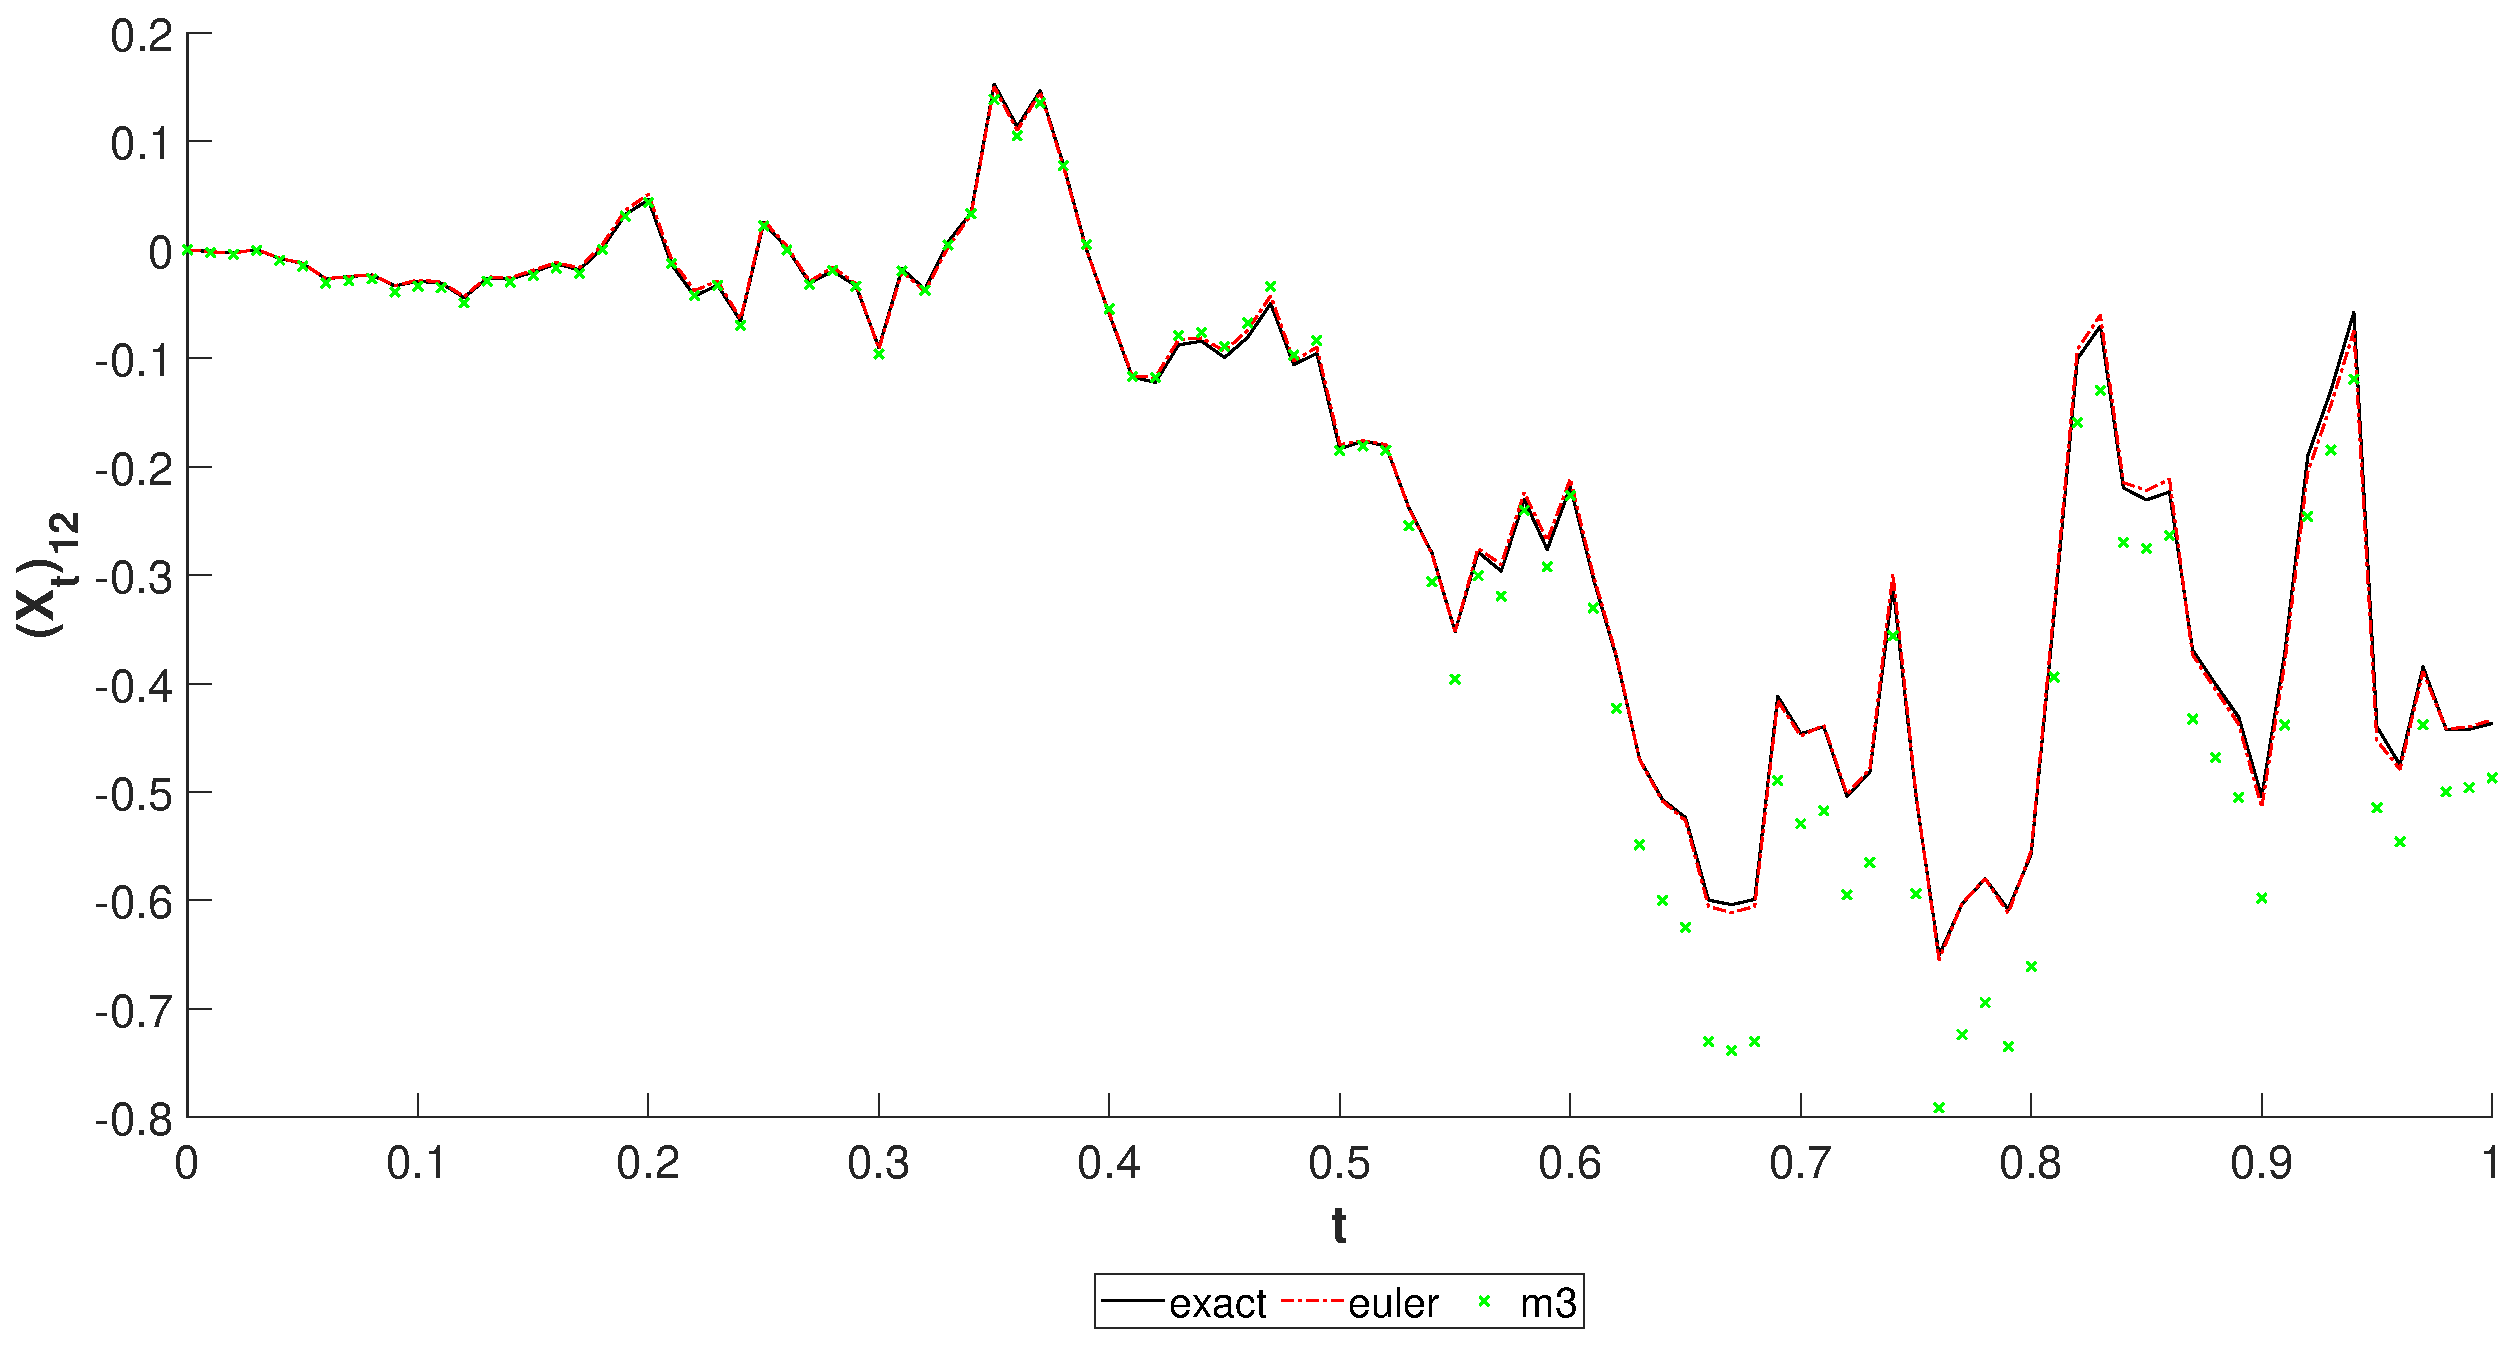
\includegraphics[width=.95\columnwidth]{C:/Users/kevin/Documents/MATLAB/PhD/Magnus/Final/Correction/B0_var/Pdf/temp/plot_8.eps}
\end{landscape}
\begin{landscape}
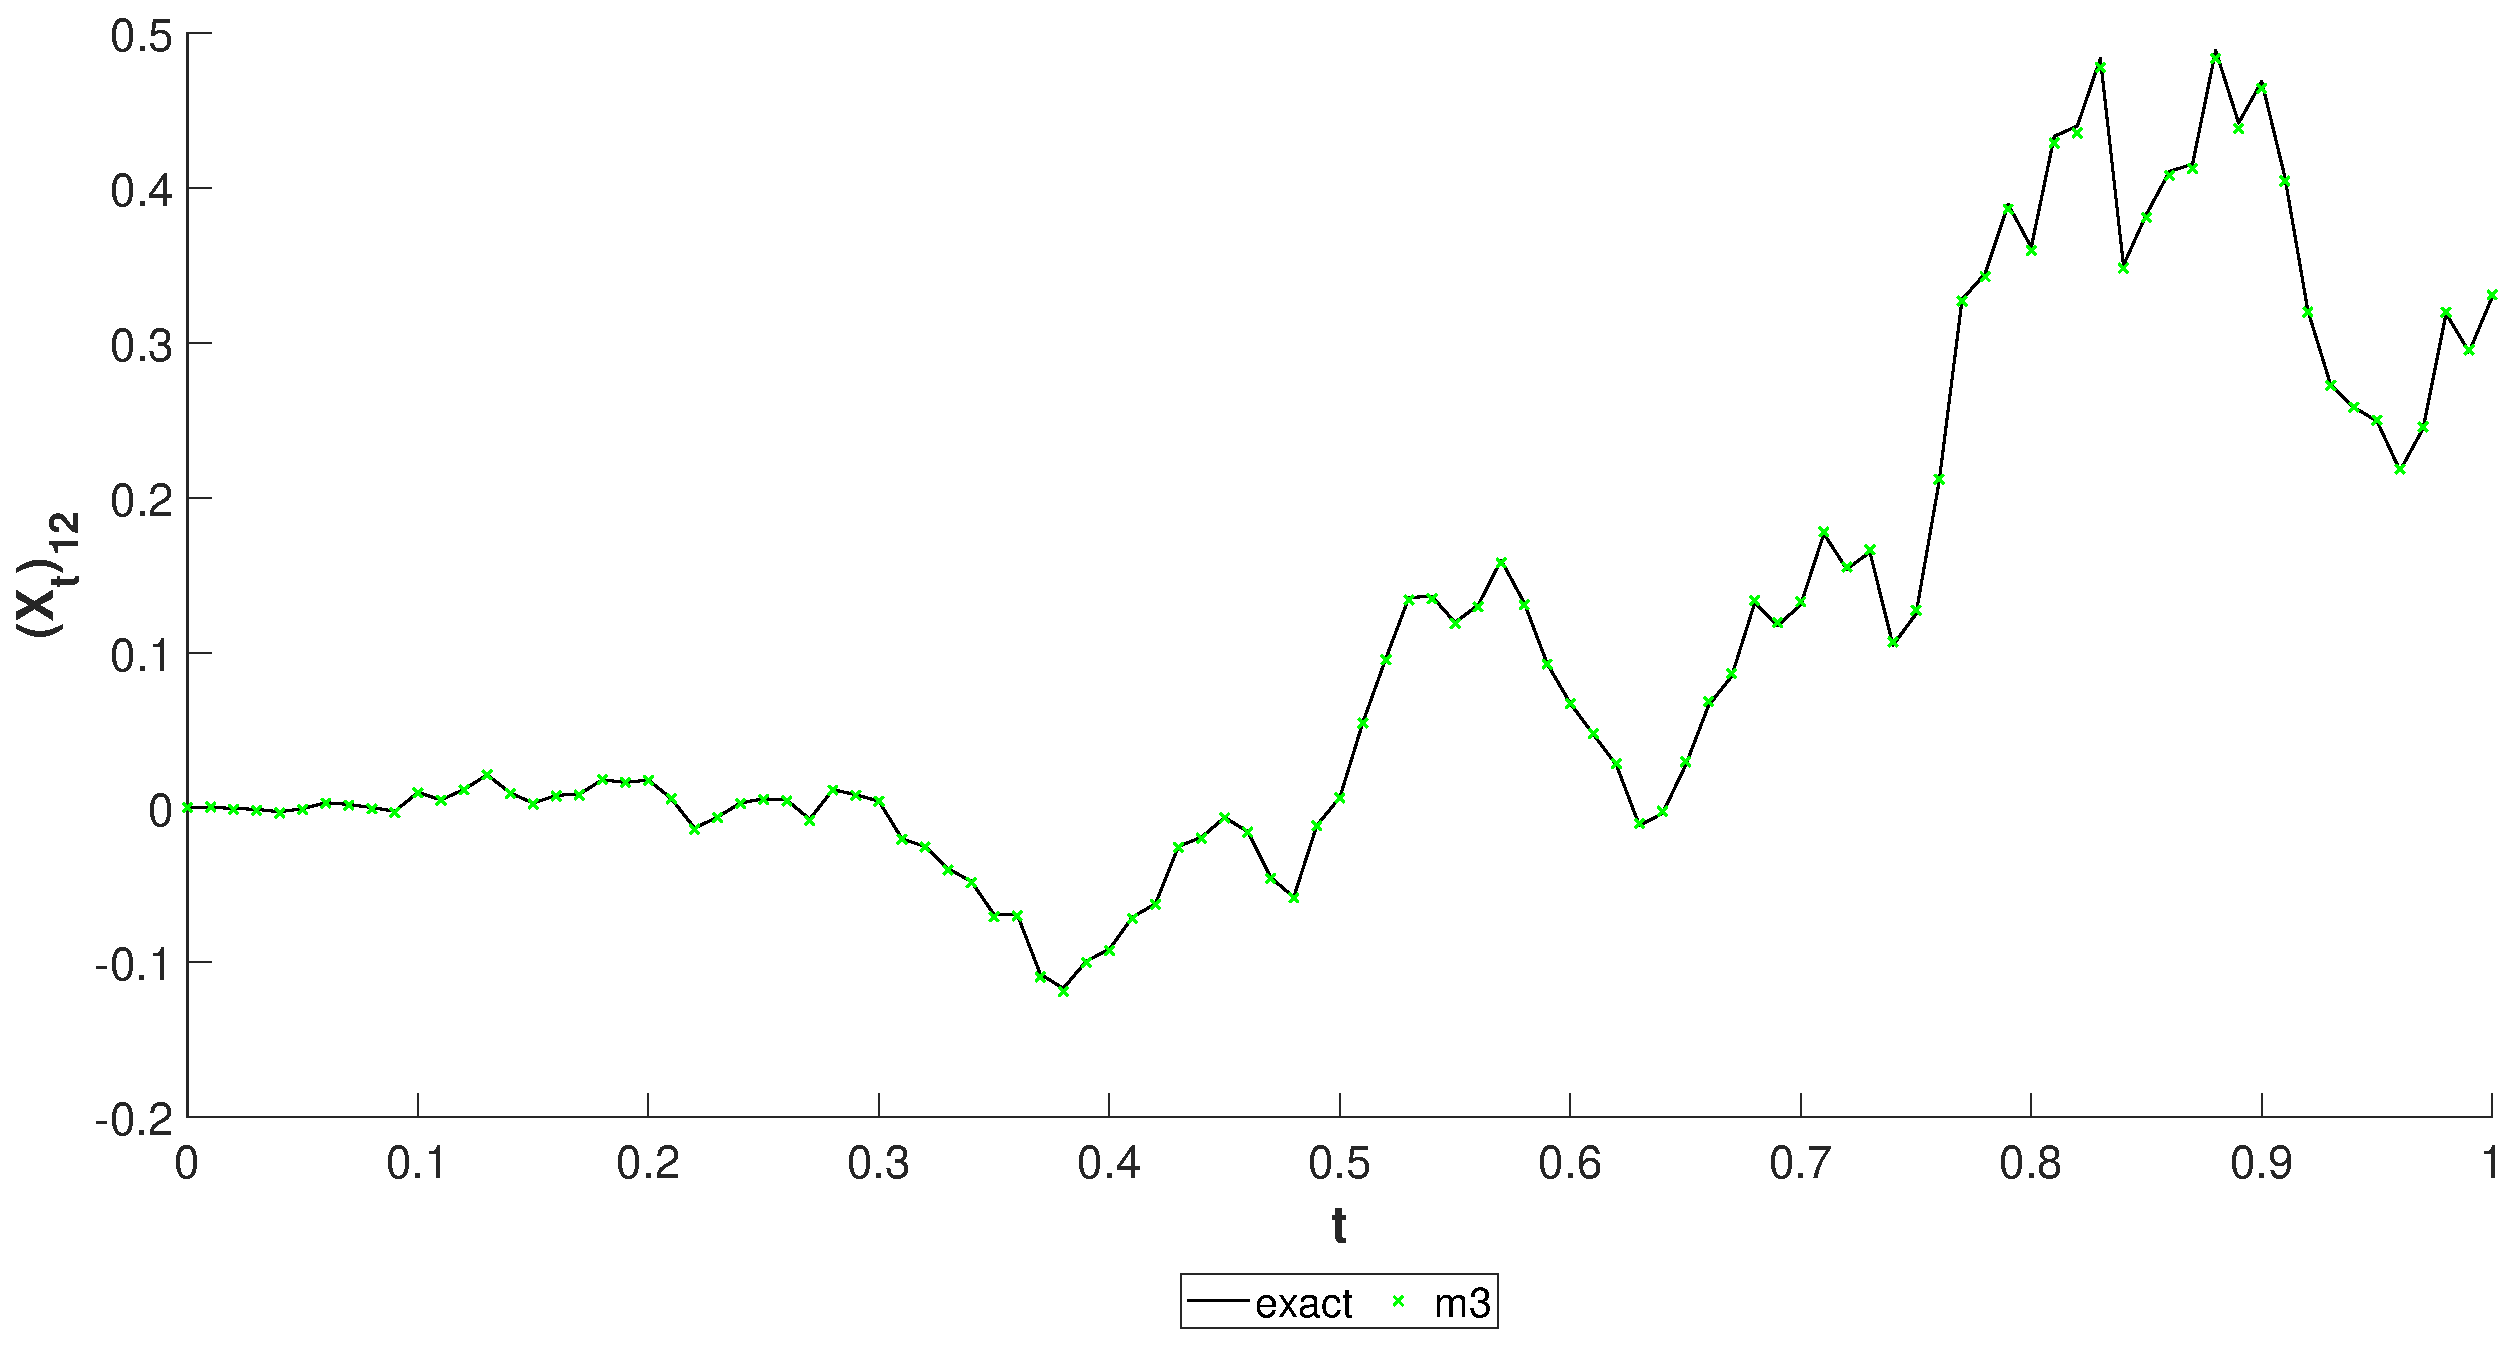
\includegraphics[width=.95\columnwidth]{C:/Users/kevin/Documents/MATLAB/PhD/Magnus/Final/Correction/B0_var/Pdf/temp/plot_9.eps}
\end{landscape}
\begin{landscape}
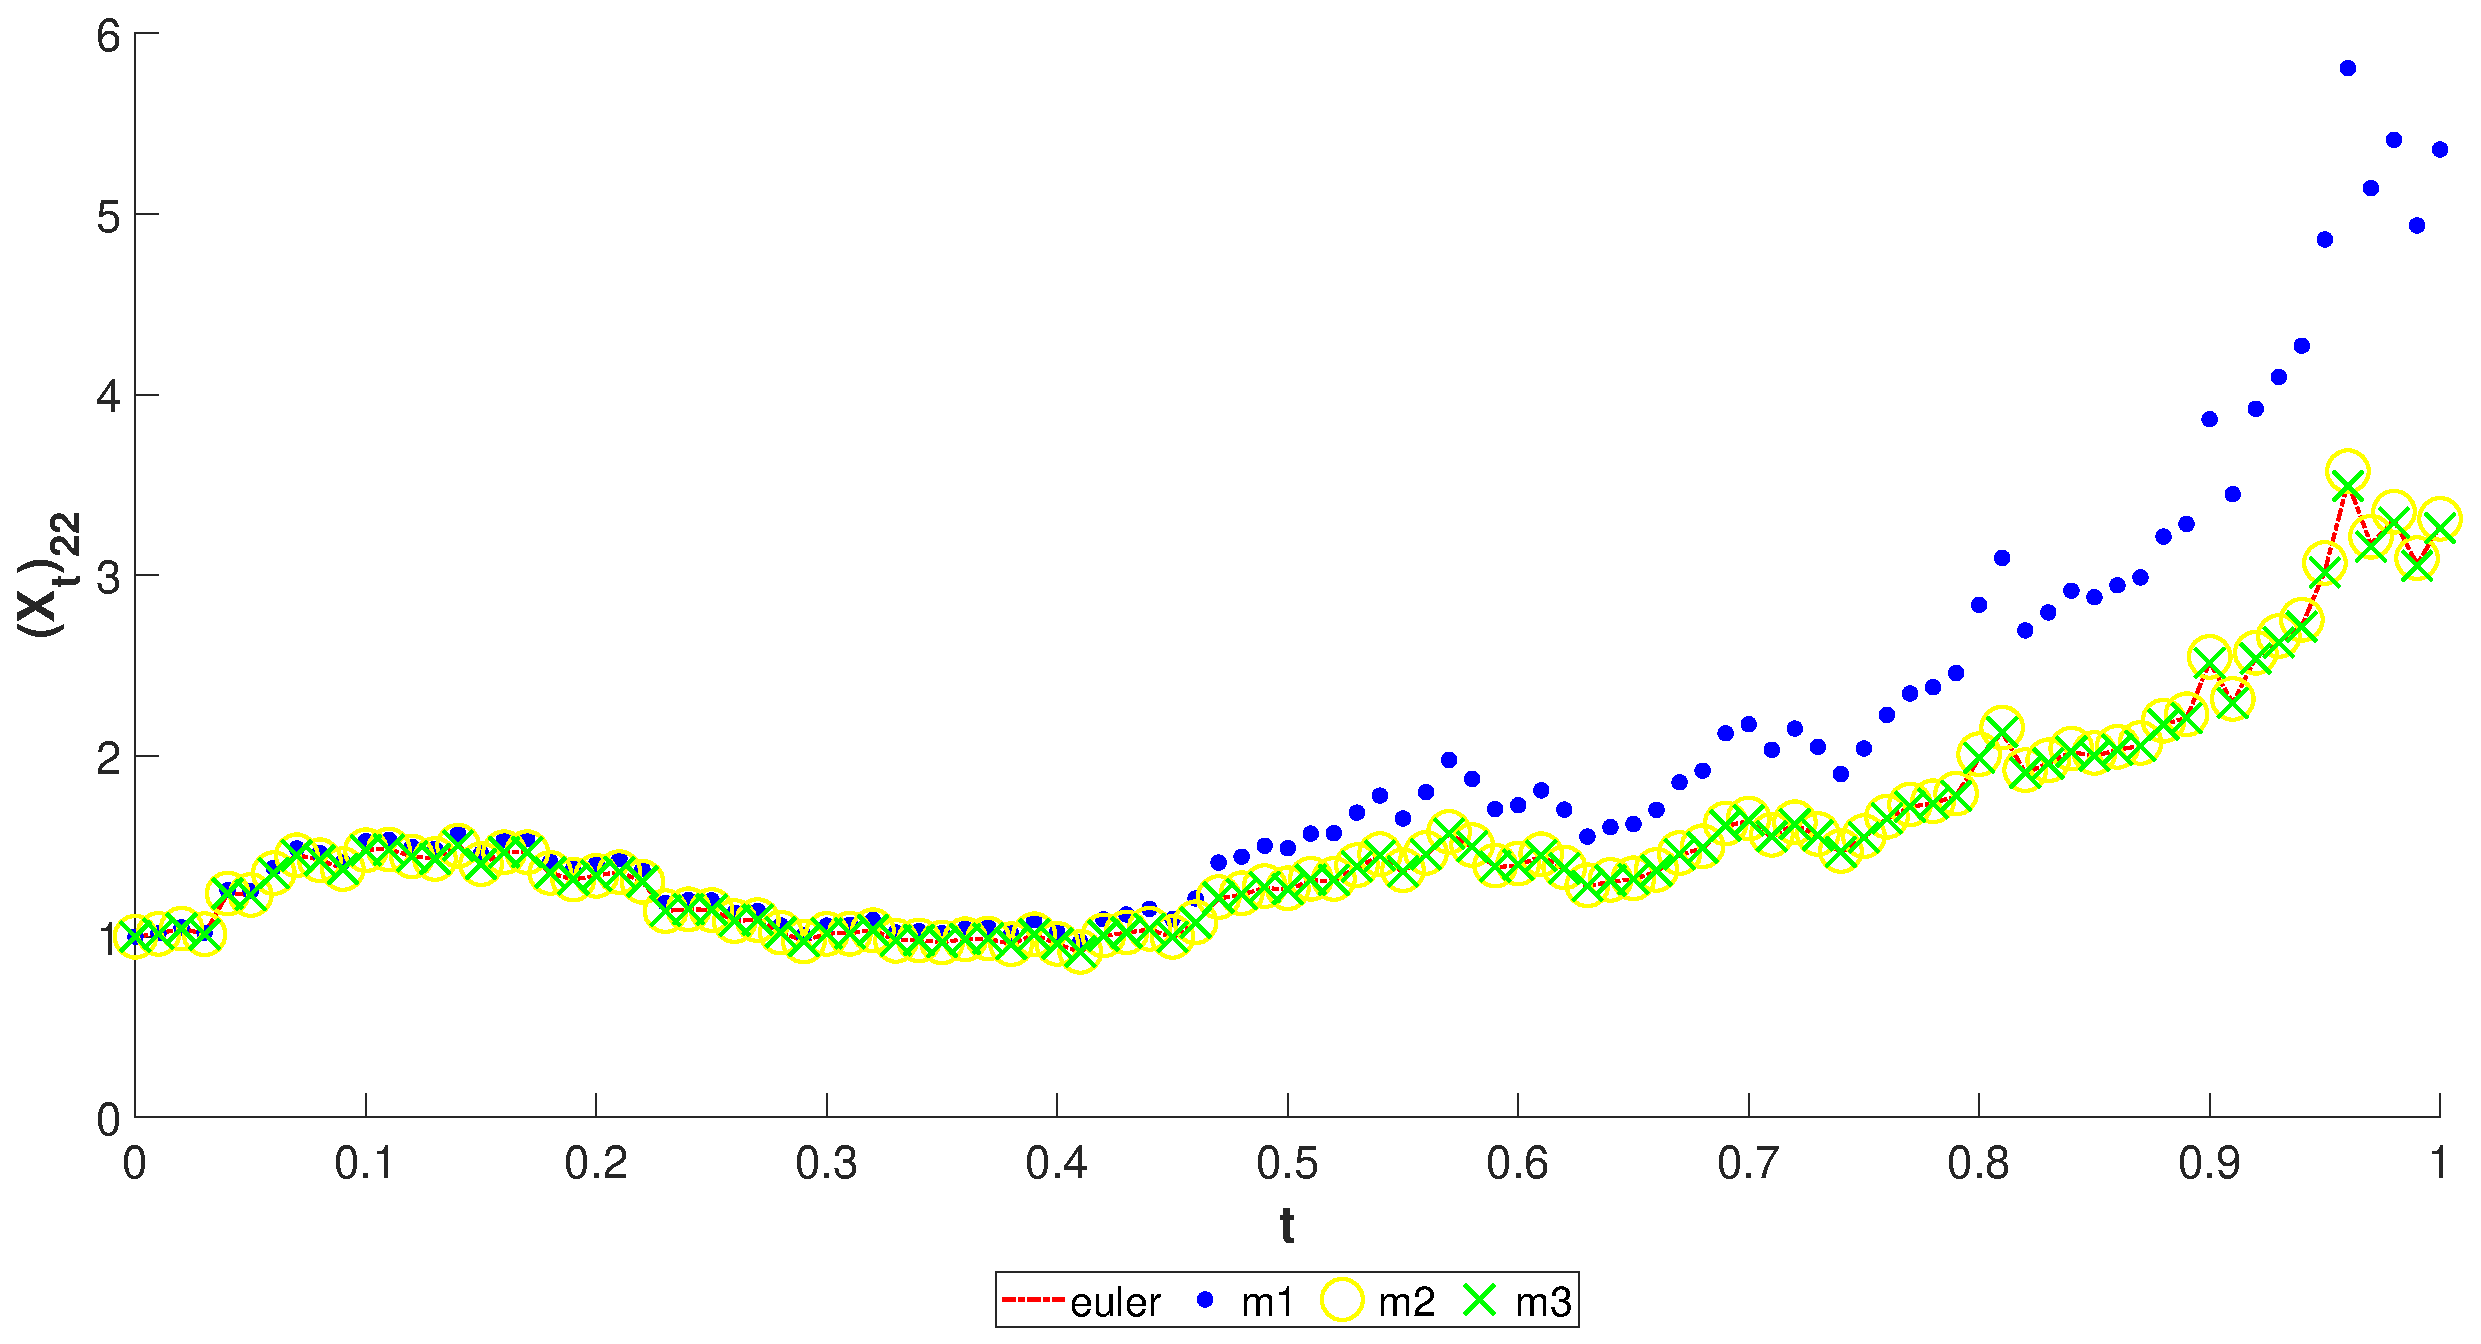
\includegraphics[width=.95\columnwidth]{C:/Users/kevin/Documents/MATLAB/PhD/Magnus/Final/Correction/B0_var/Pdf/temp/plot_10.eps}
\end{landscape}
\begin{landscape}
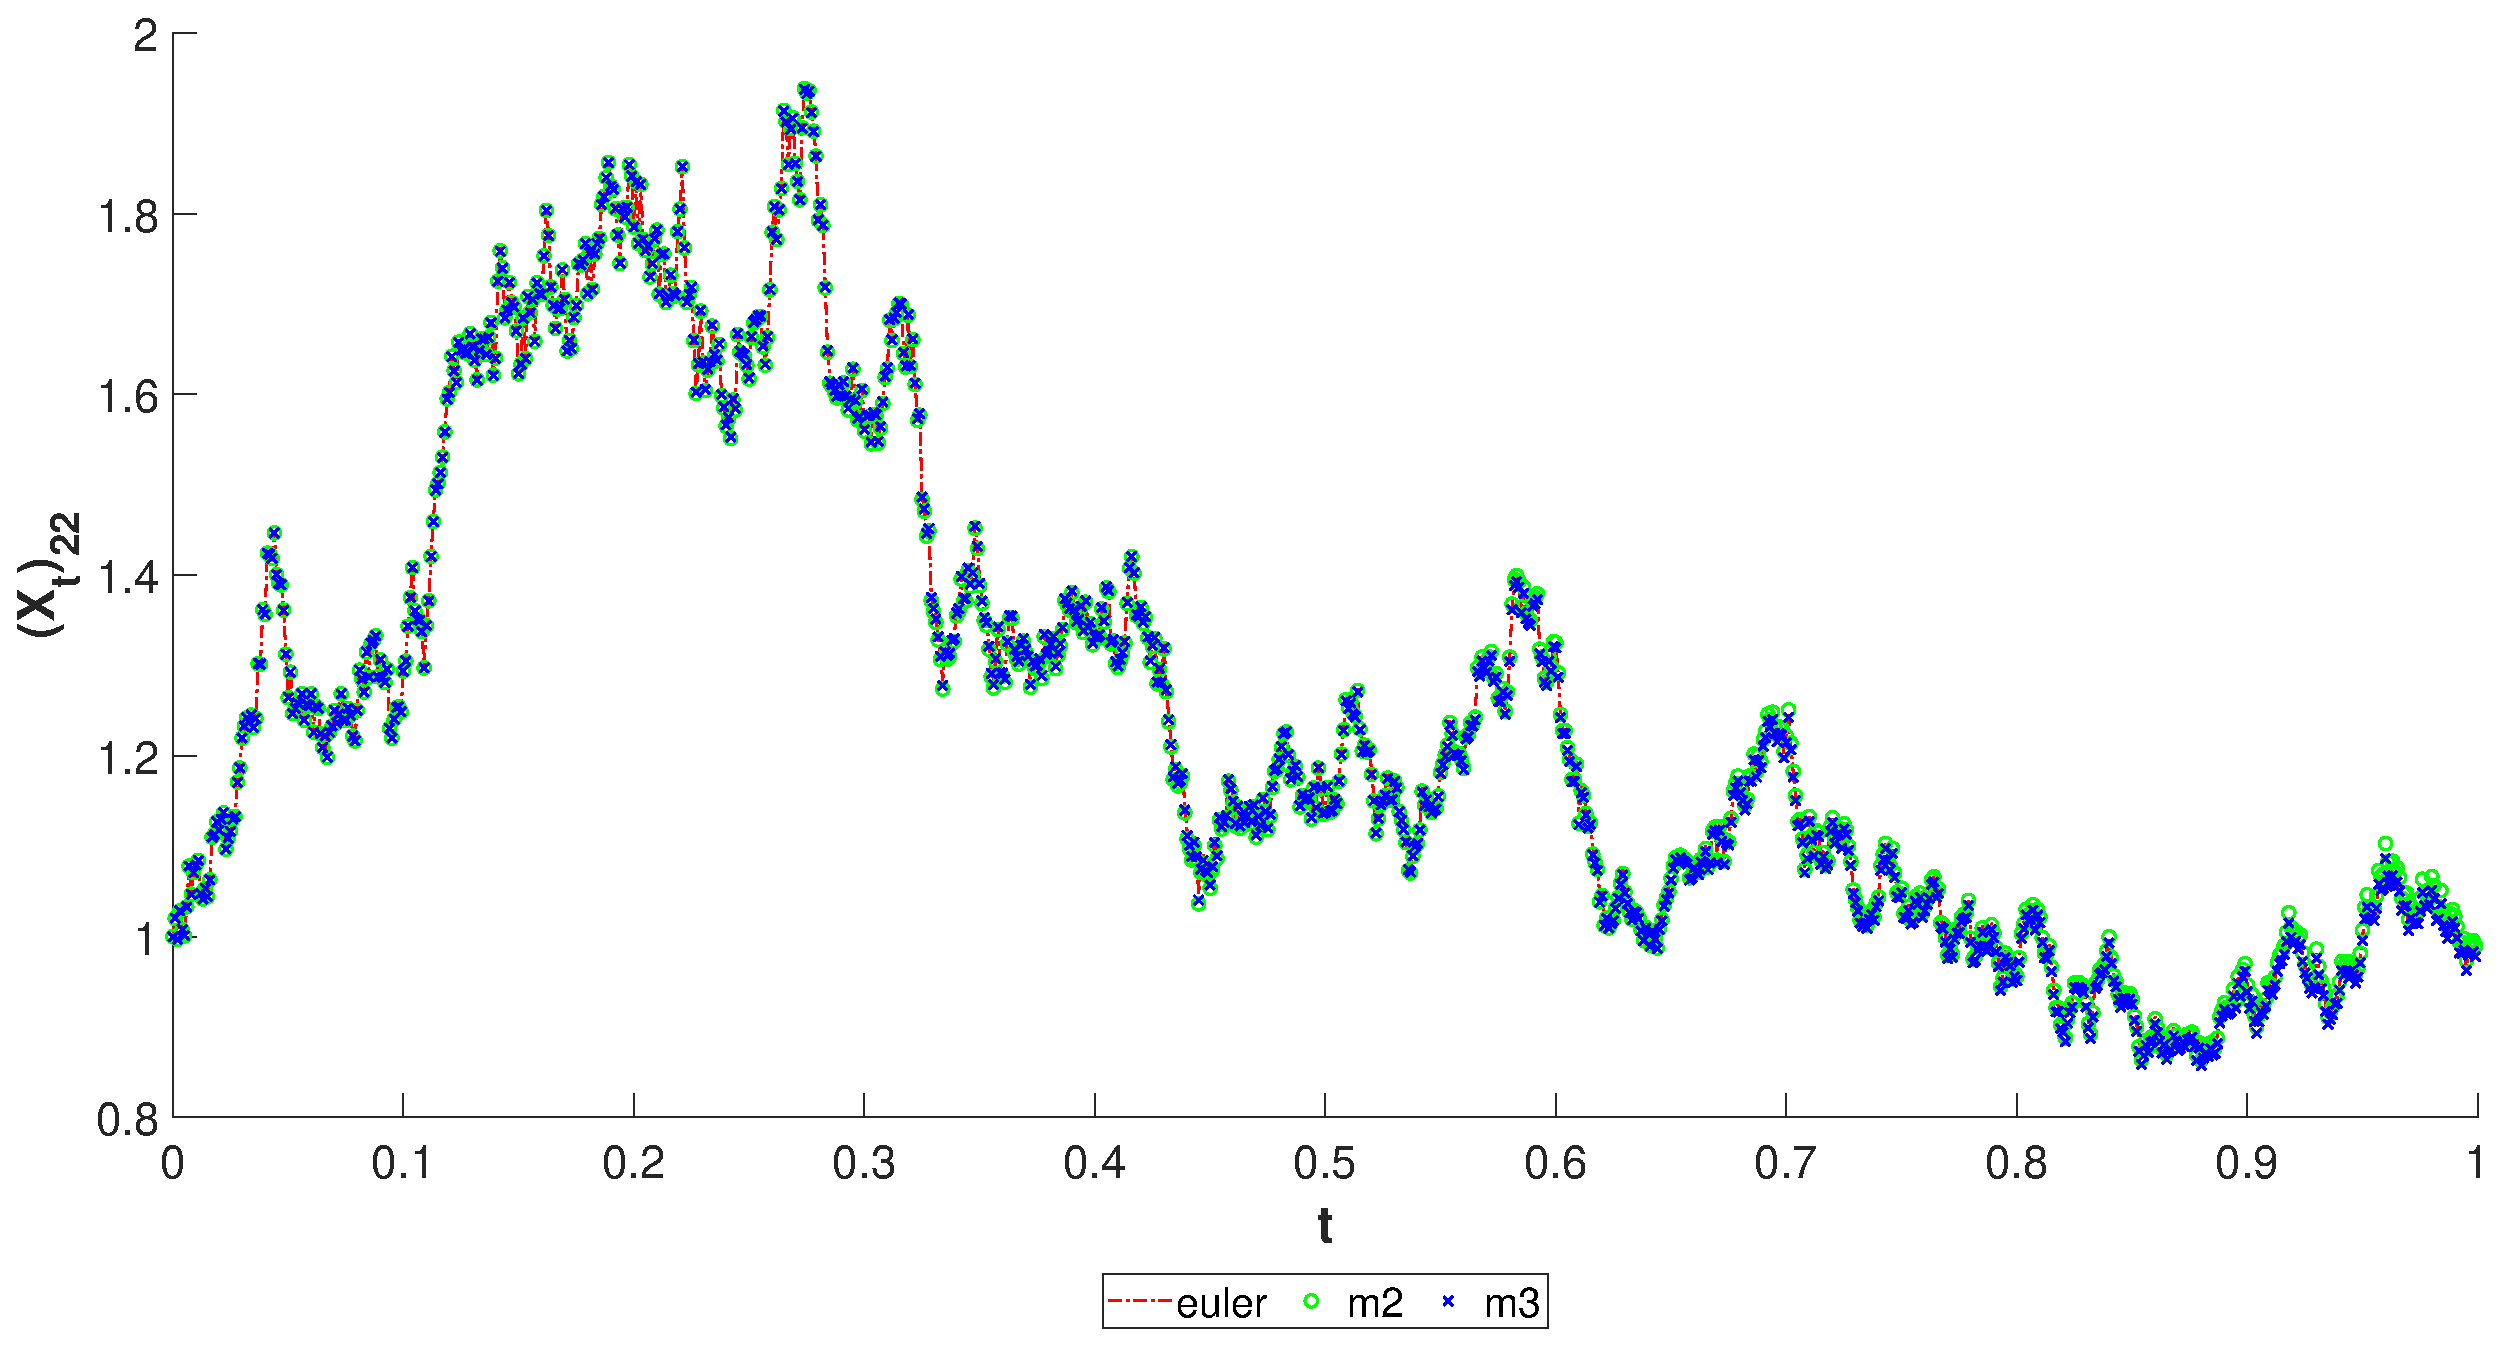
\includegraphics[width=.95\columnwidth]{C:/Users/kevin/Documents/MATLAB/PhD/Magnus/Final/Correction/B0_var/Pdf/temp/plot_11.eps}
\end{landscape}
\begin{landscape}
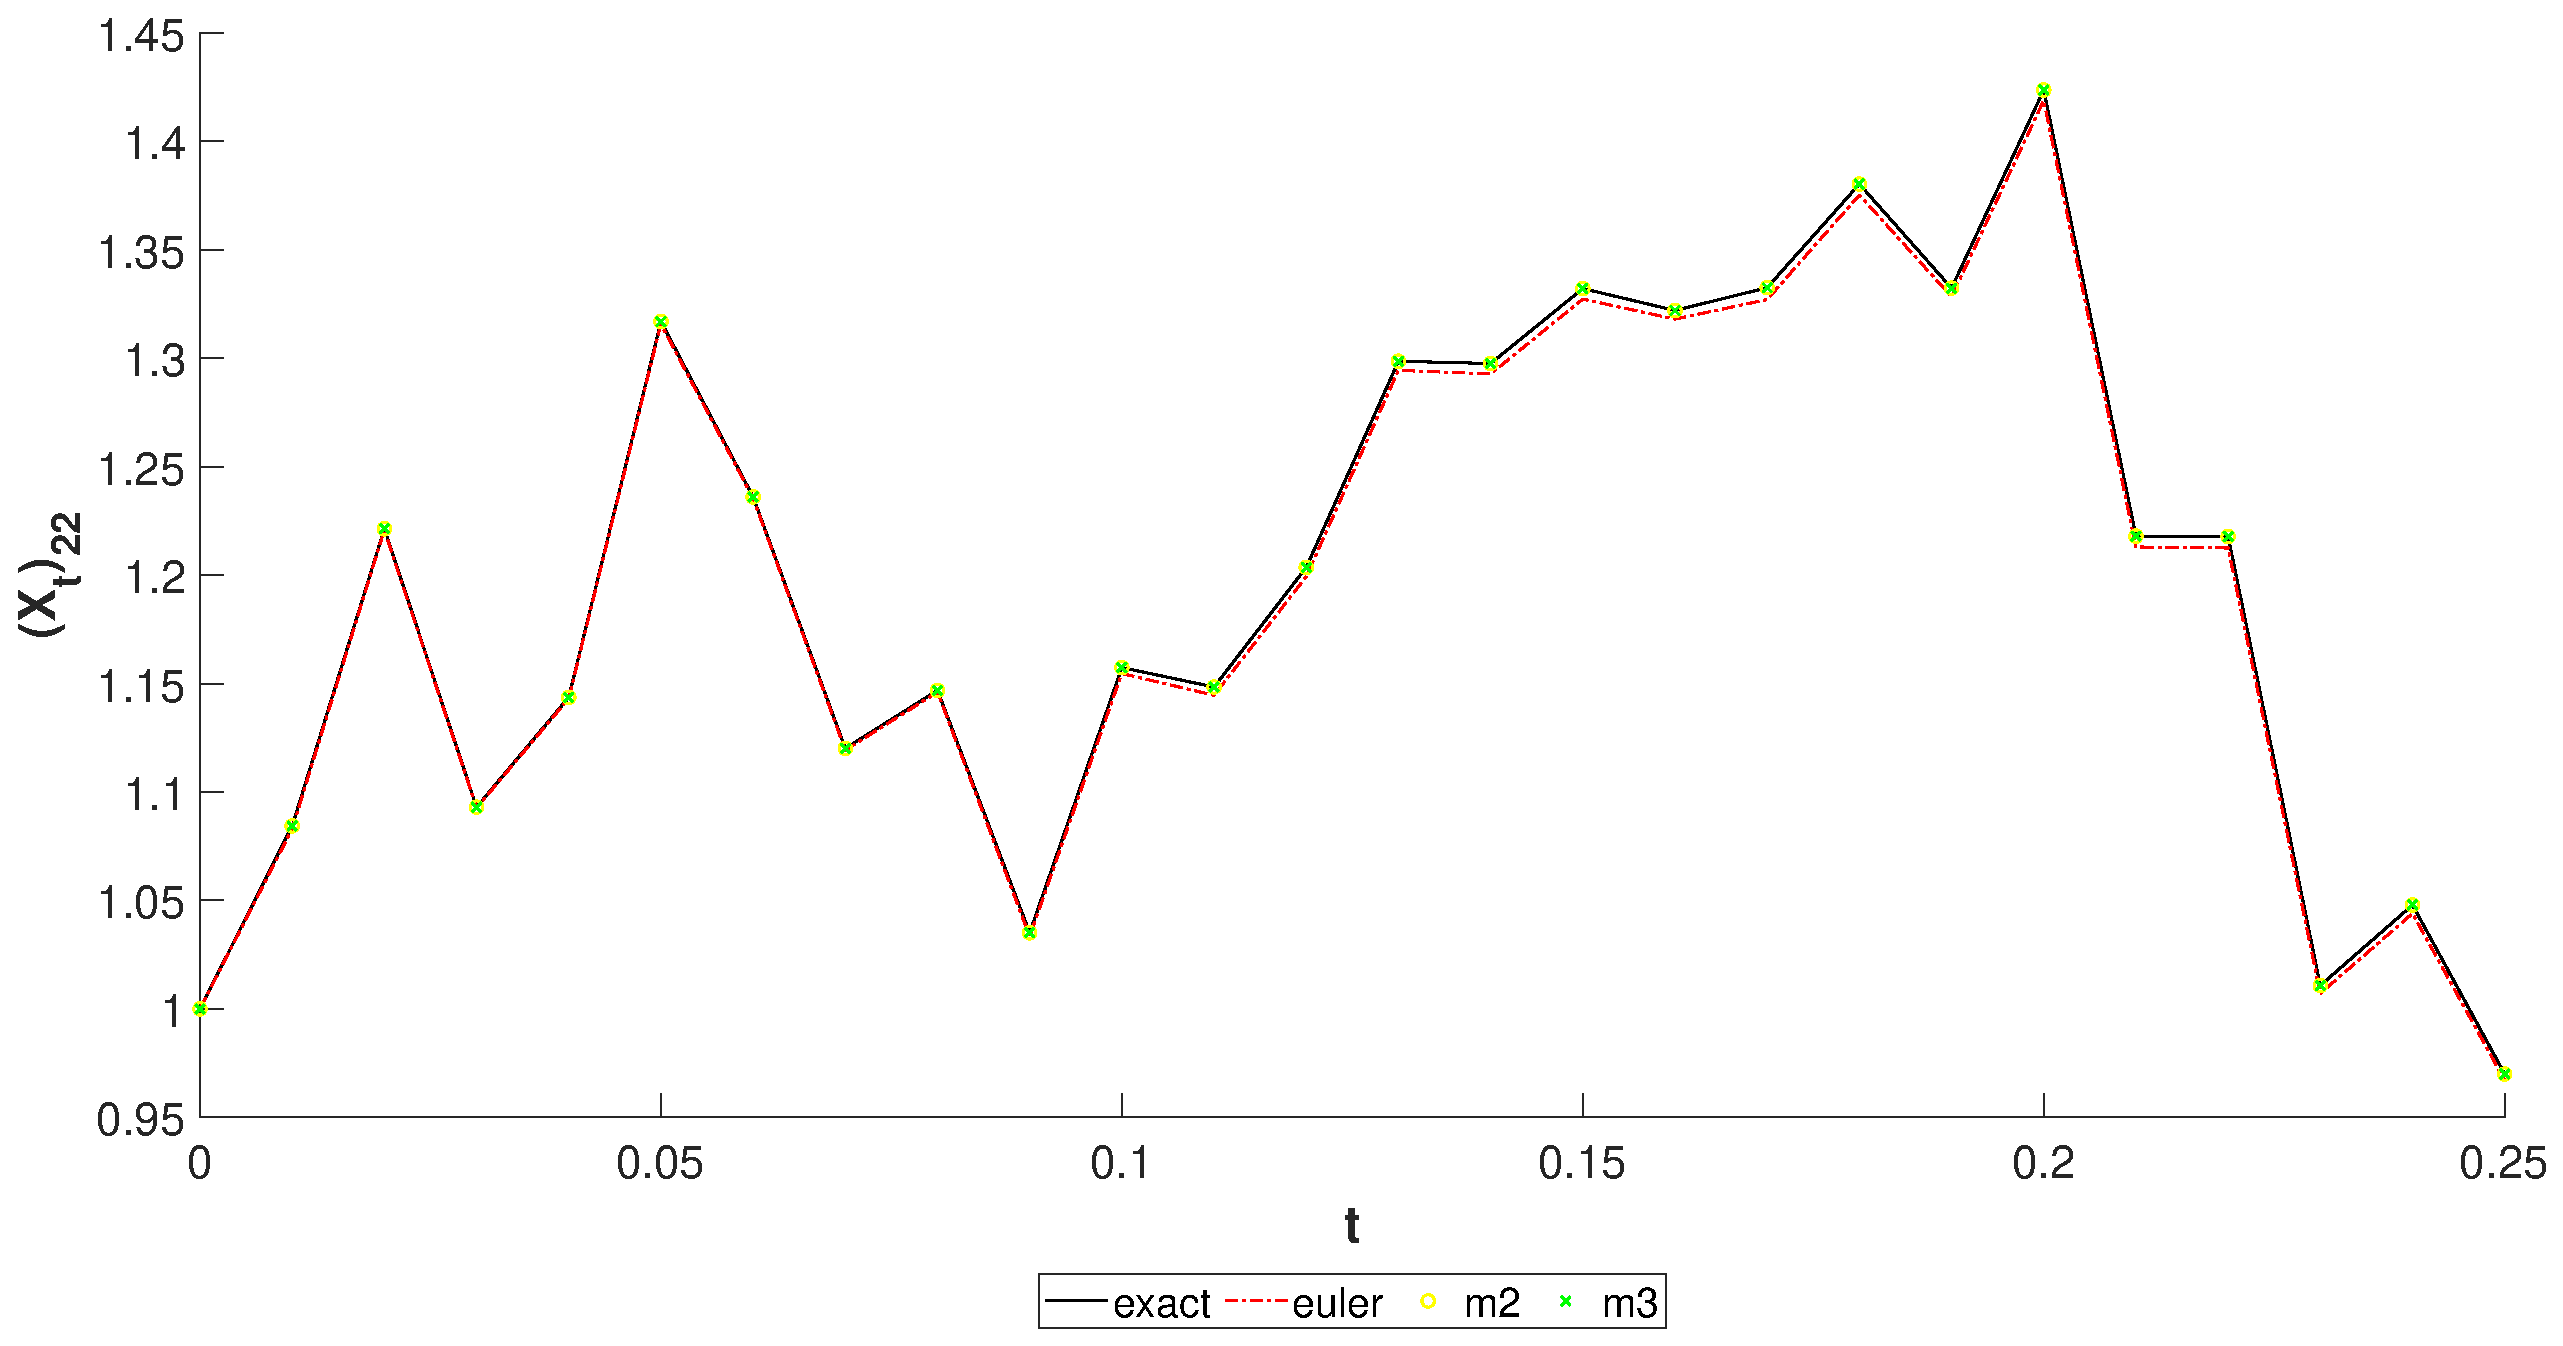
\includegraphics[width=.95\columnwidth]{C:/Users/kevin/Documents/MATLAB/PhD/Magnus/Final/Correction/B0_var/Pdf/temp/plot_12.eps}
\end{landscape}
\begin{landscape}
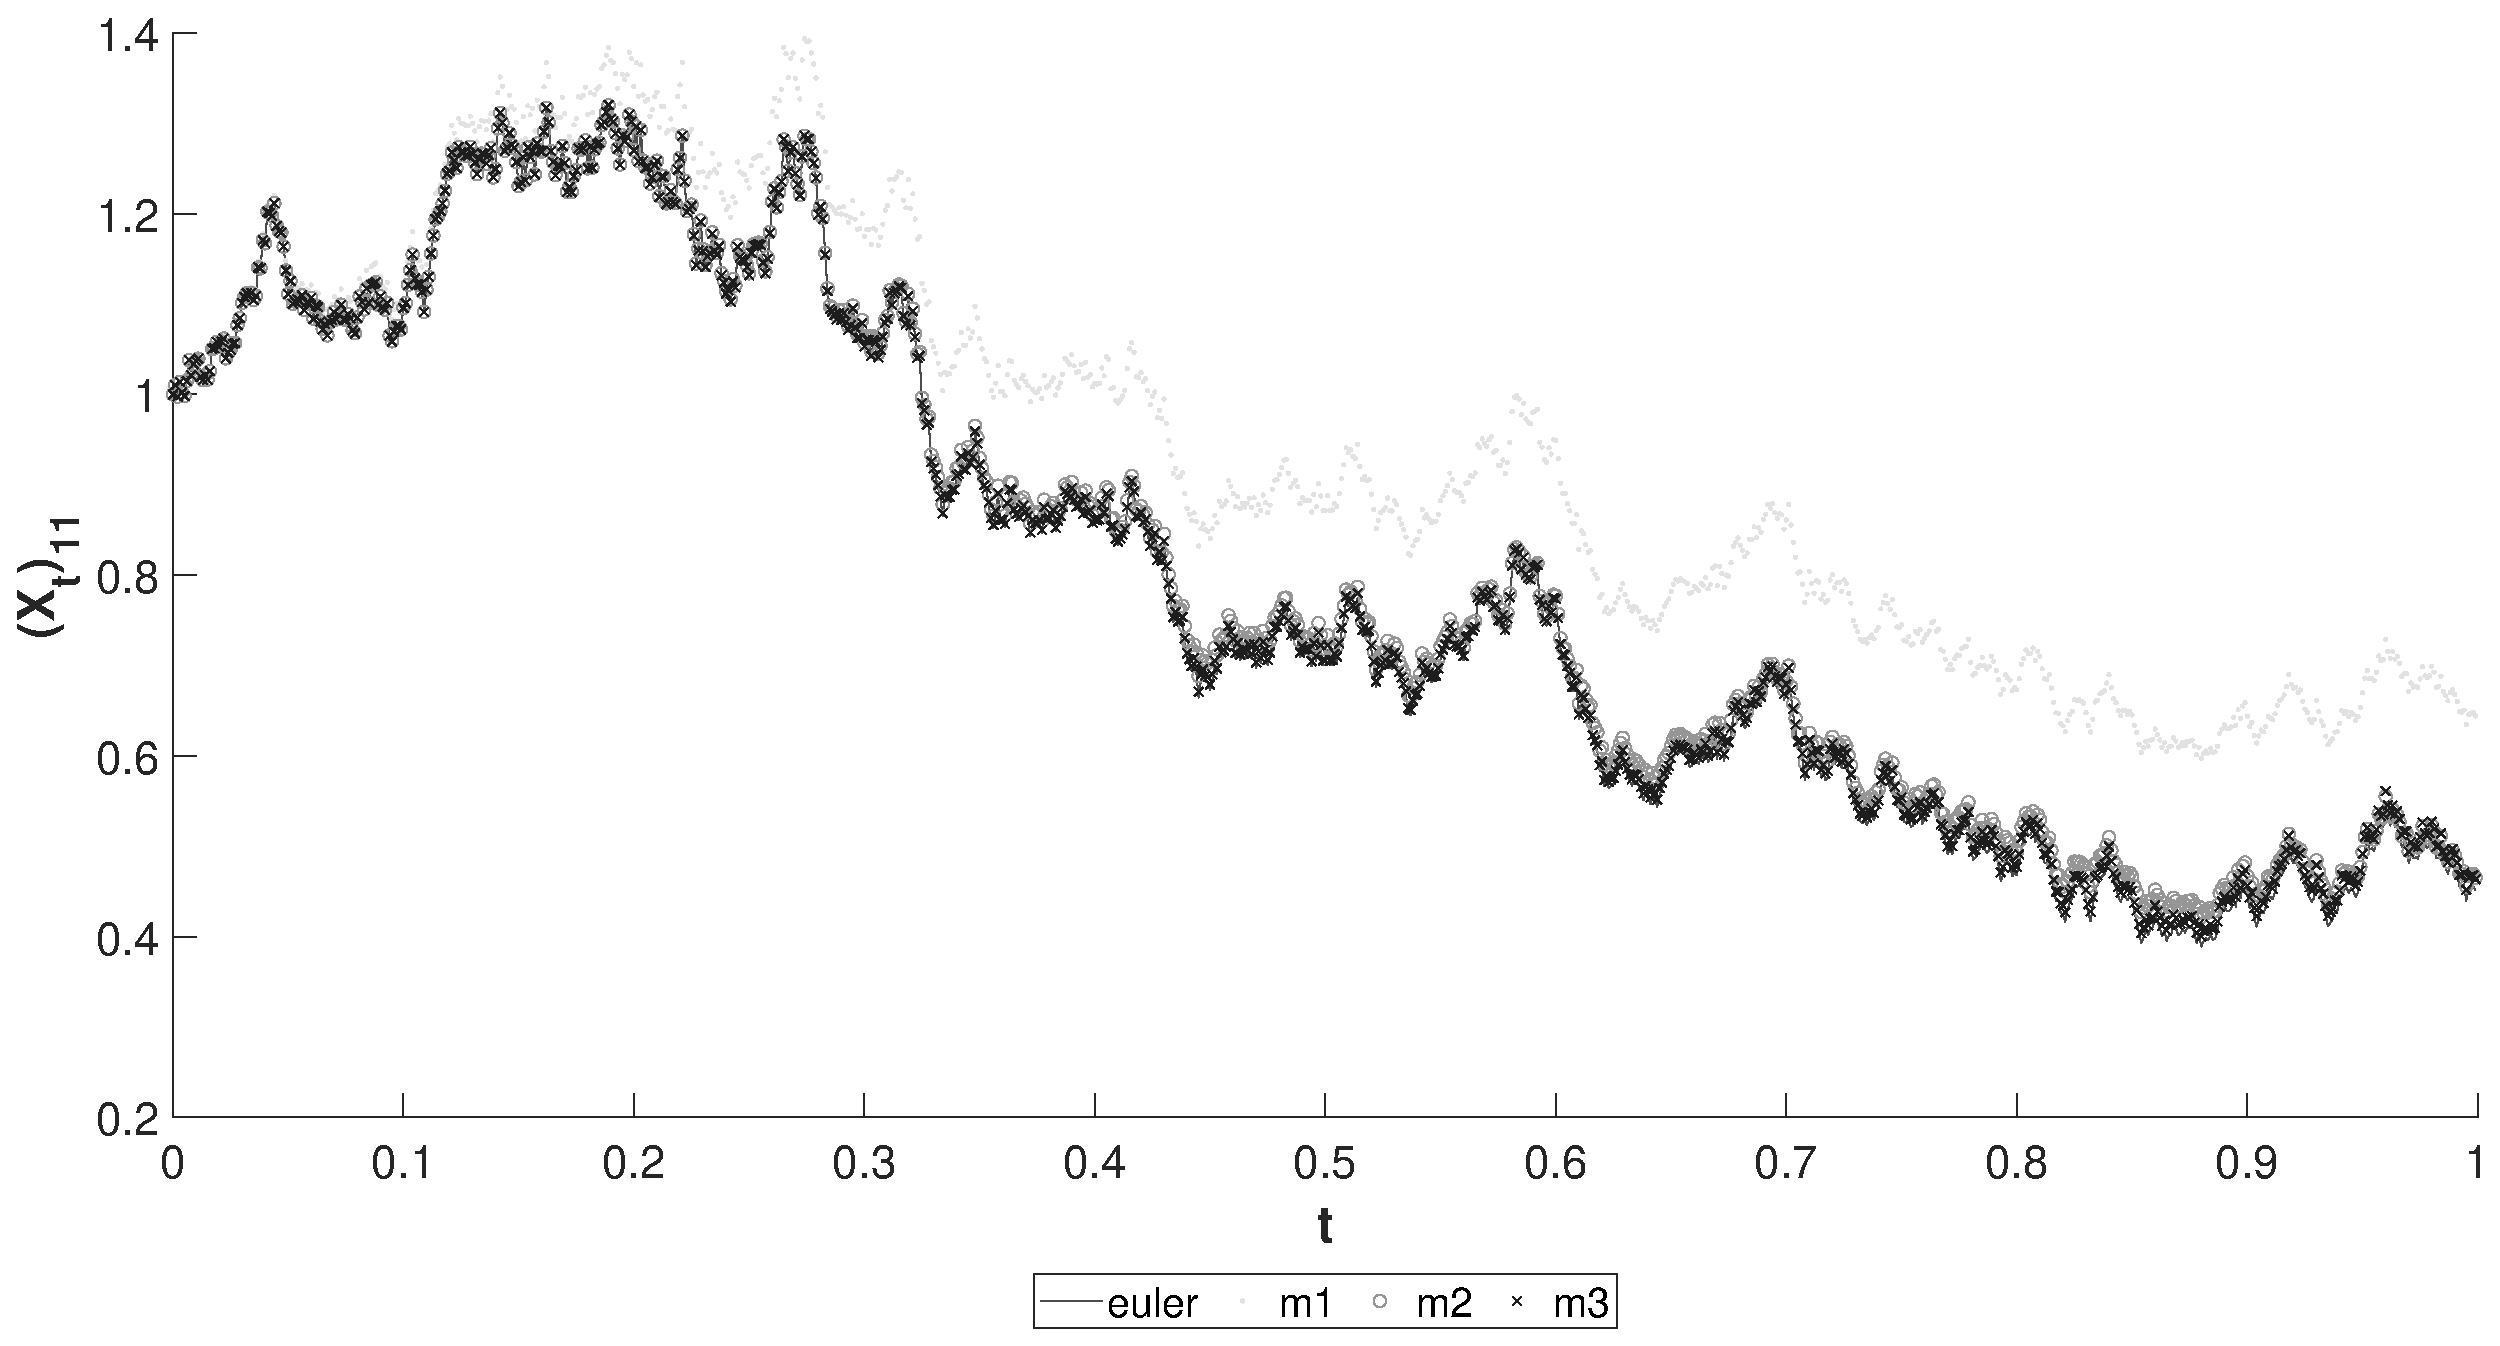
\includegraphics[width=.95\columnwidth]{C:/Users/kevin/Documents/MATLAB/PhD/Magnus/Final/Correction/B0_var/Pdf/temp/plot_13.eps}
\end{landscape}
\begin{landscape}
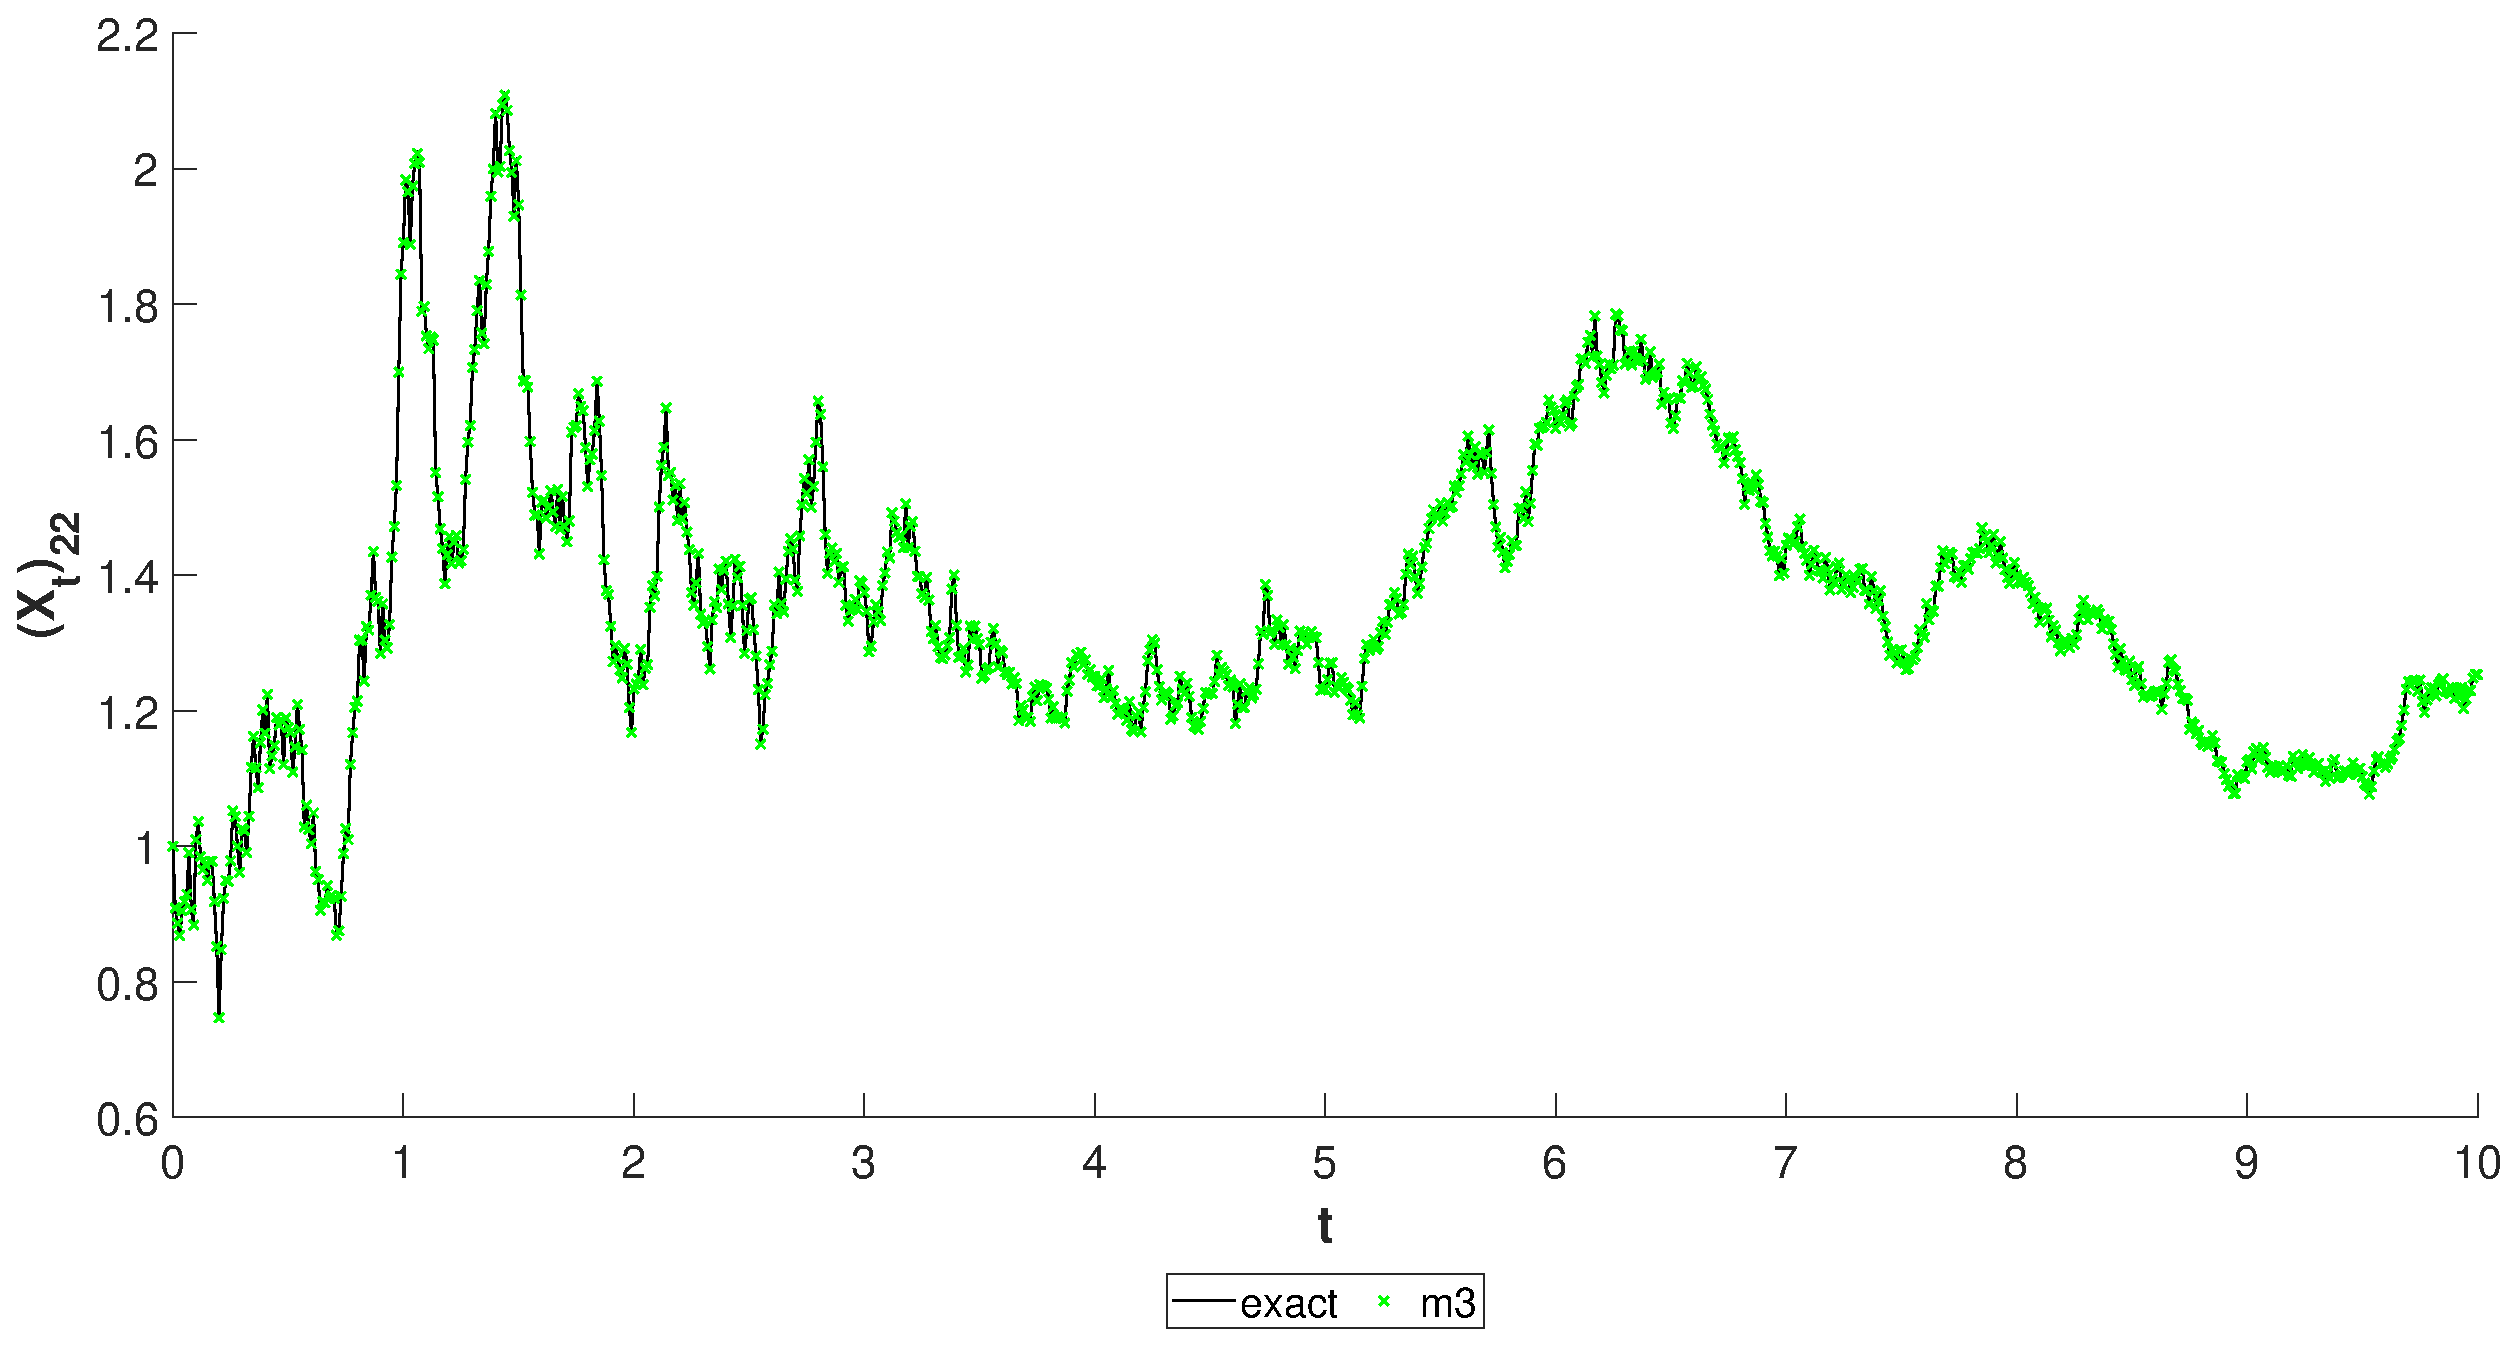
\includegraphics[width=.95\columnwidth]{C:/Users/kevin/Documents/MATLAB/PhD/Magnus/Final/Correction/B0_var/Pdf/temp/plot_14.eps}
\end{landscape}
\begin{landscape}
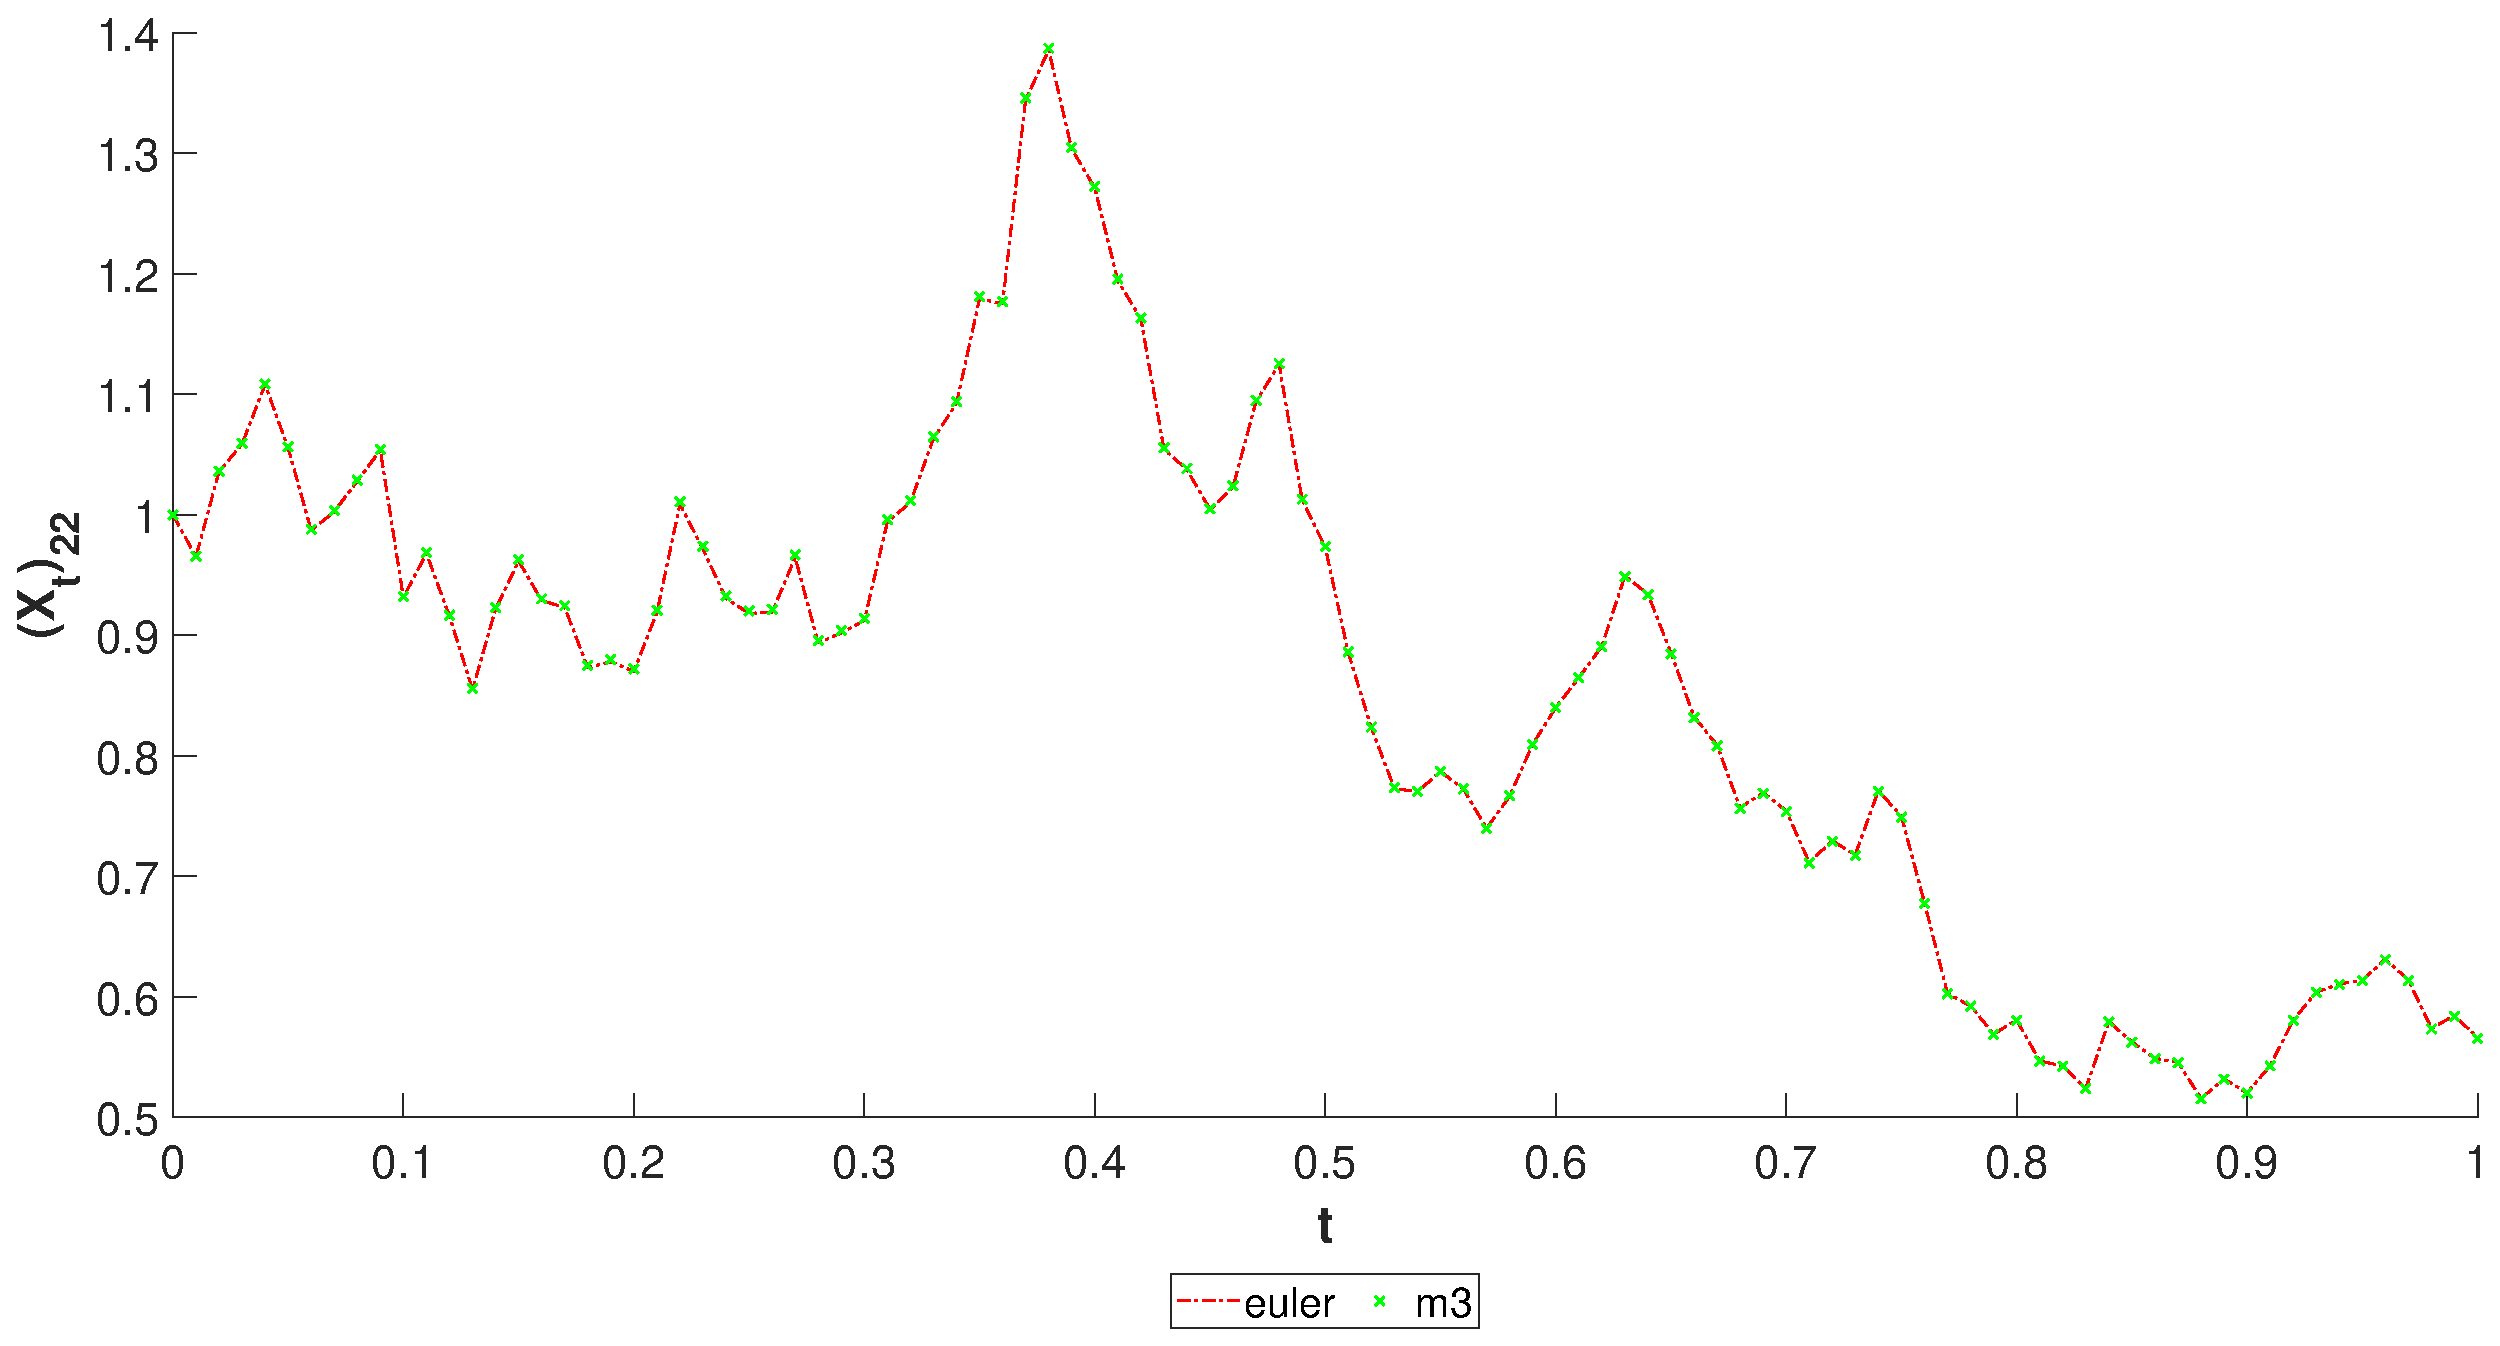
\includegraphics[width=.95\columnwidth]{C:/Users/kevin/Documents/MATLAB/PhD/Magnus/Final/Correction/B0_var/Pdf/temp/plot_15.eps}
\end{landscape}

\subsection{Error Plots}
	\begin{landscape}
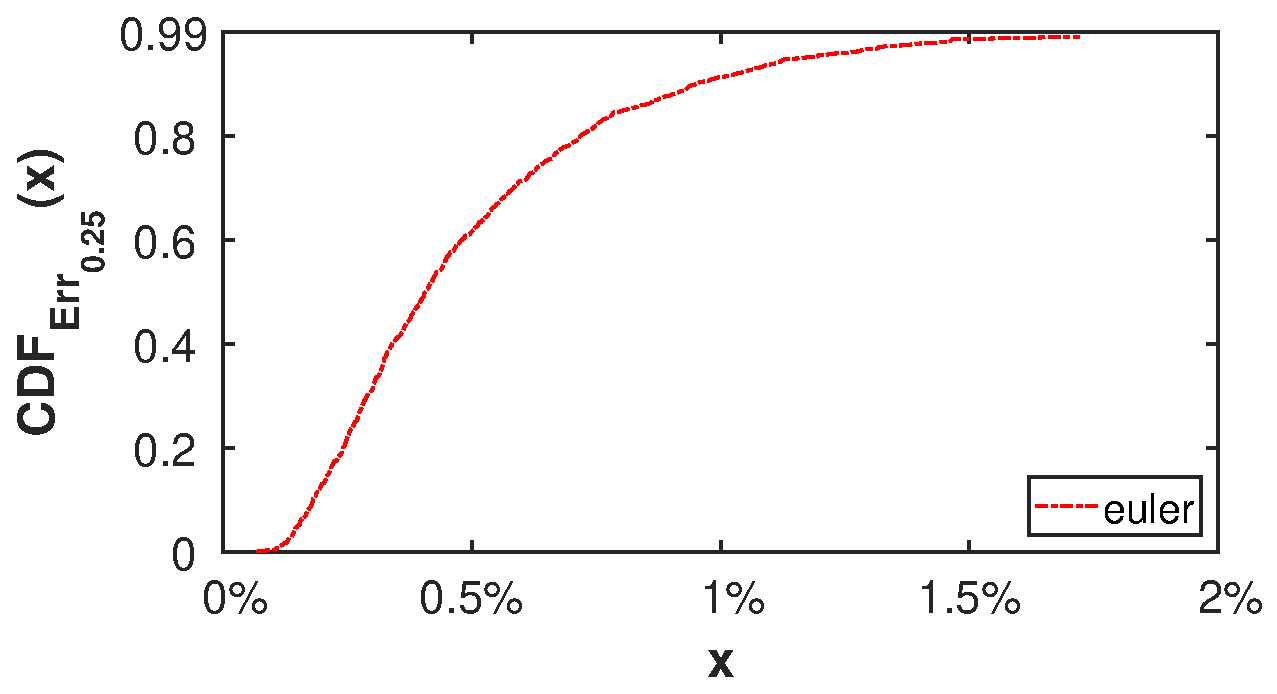
\includegraphics[width=.95\columnwidth]{C:/Users/kevin/Documents/MATLAB/PhD/Magnus/Final/Correction/B0_var/Pdf/temp/error_plot_1.eps}
\end{landscape}
\begin{landscape}
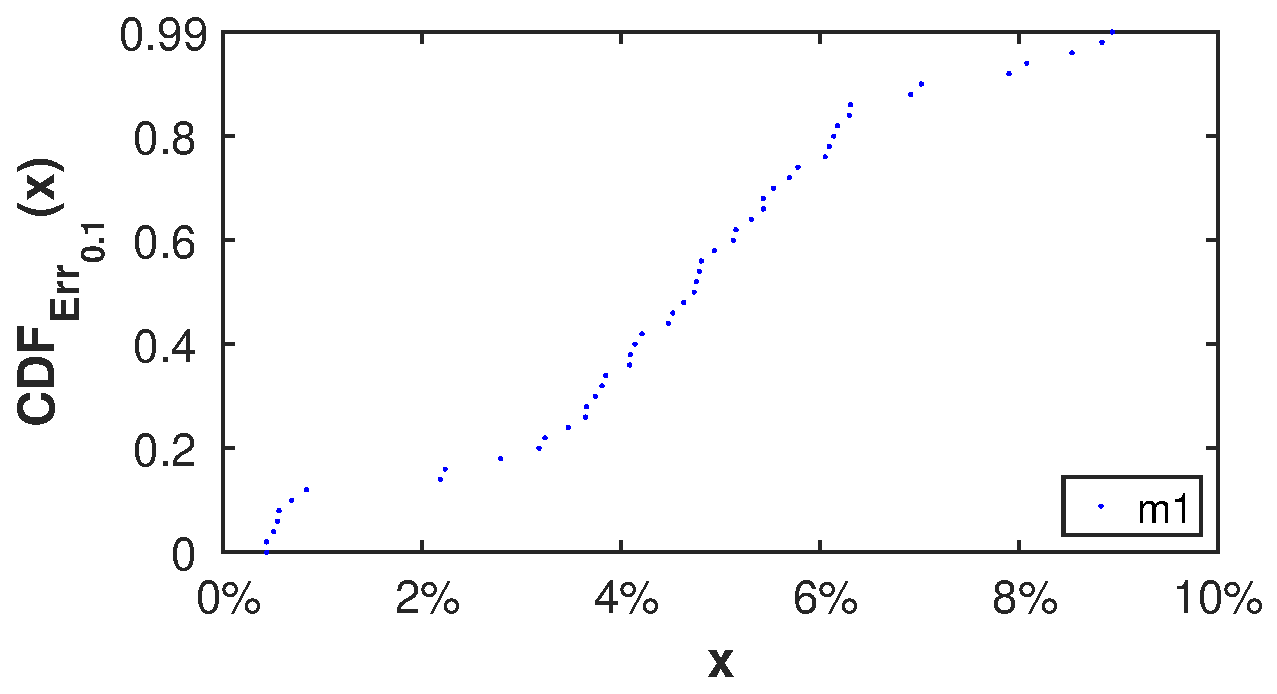
\includegraphics[width=.95\columnwidth]{C:/Users/kevin/Documents/MATLAB/PhD/Magnus/Final/Correction/B0_var/Pdf/temp/error_plot_2.eps}
\end{landscape}
\begin{landscape}
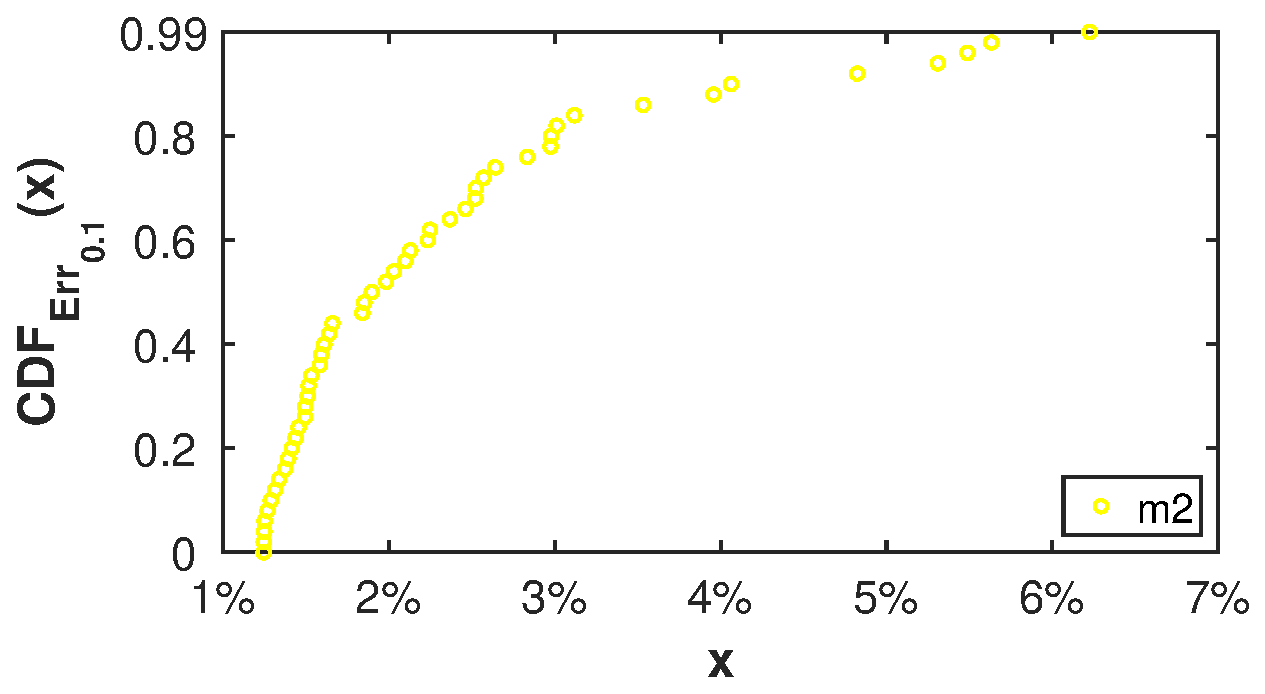
\includegraphics[width=.95\columnwidth]{C:/Users/kevin/Documents/MATLAB/PhD/Magnus/Final/Correction/B0_var/Pdf/temp/error_plot_3.eps}
\end{landscape}
\begin{landscape}
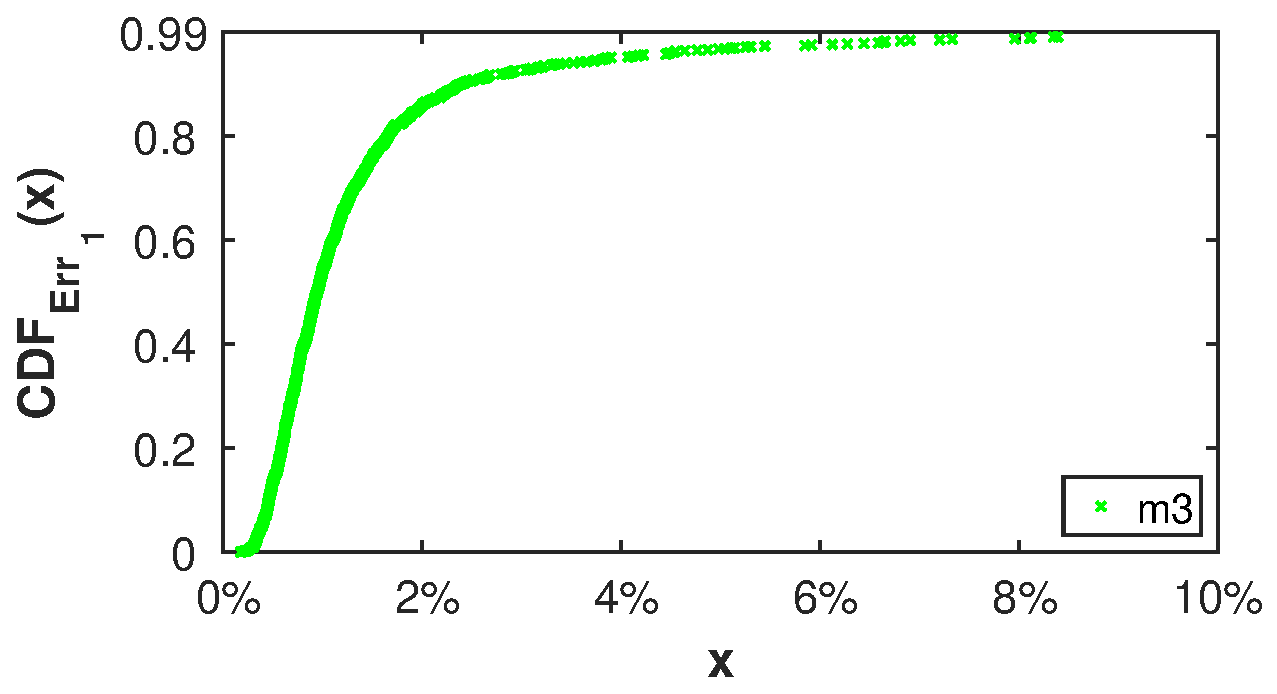
\includegraphics[width=.95\columnwidth]{C:/Users/kevin/Documents/MATLAB/PhD/Magnus/Final/Correction/B0_var/Pdf/temp/error_plot_4.eps}
\end{landscape}
\begin{landscape}
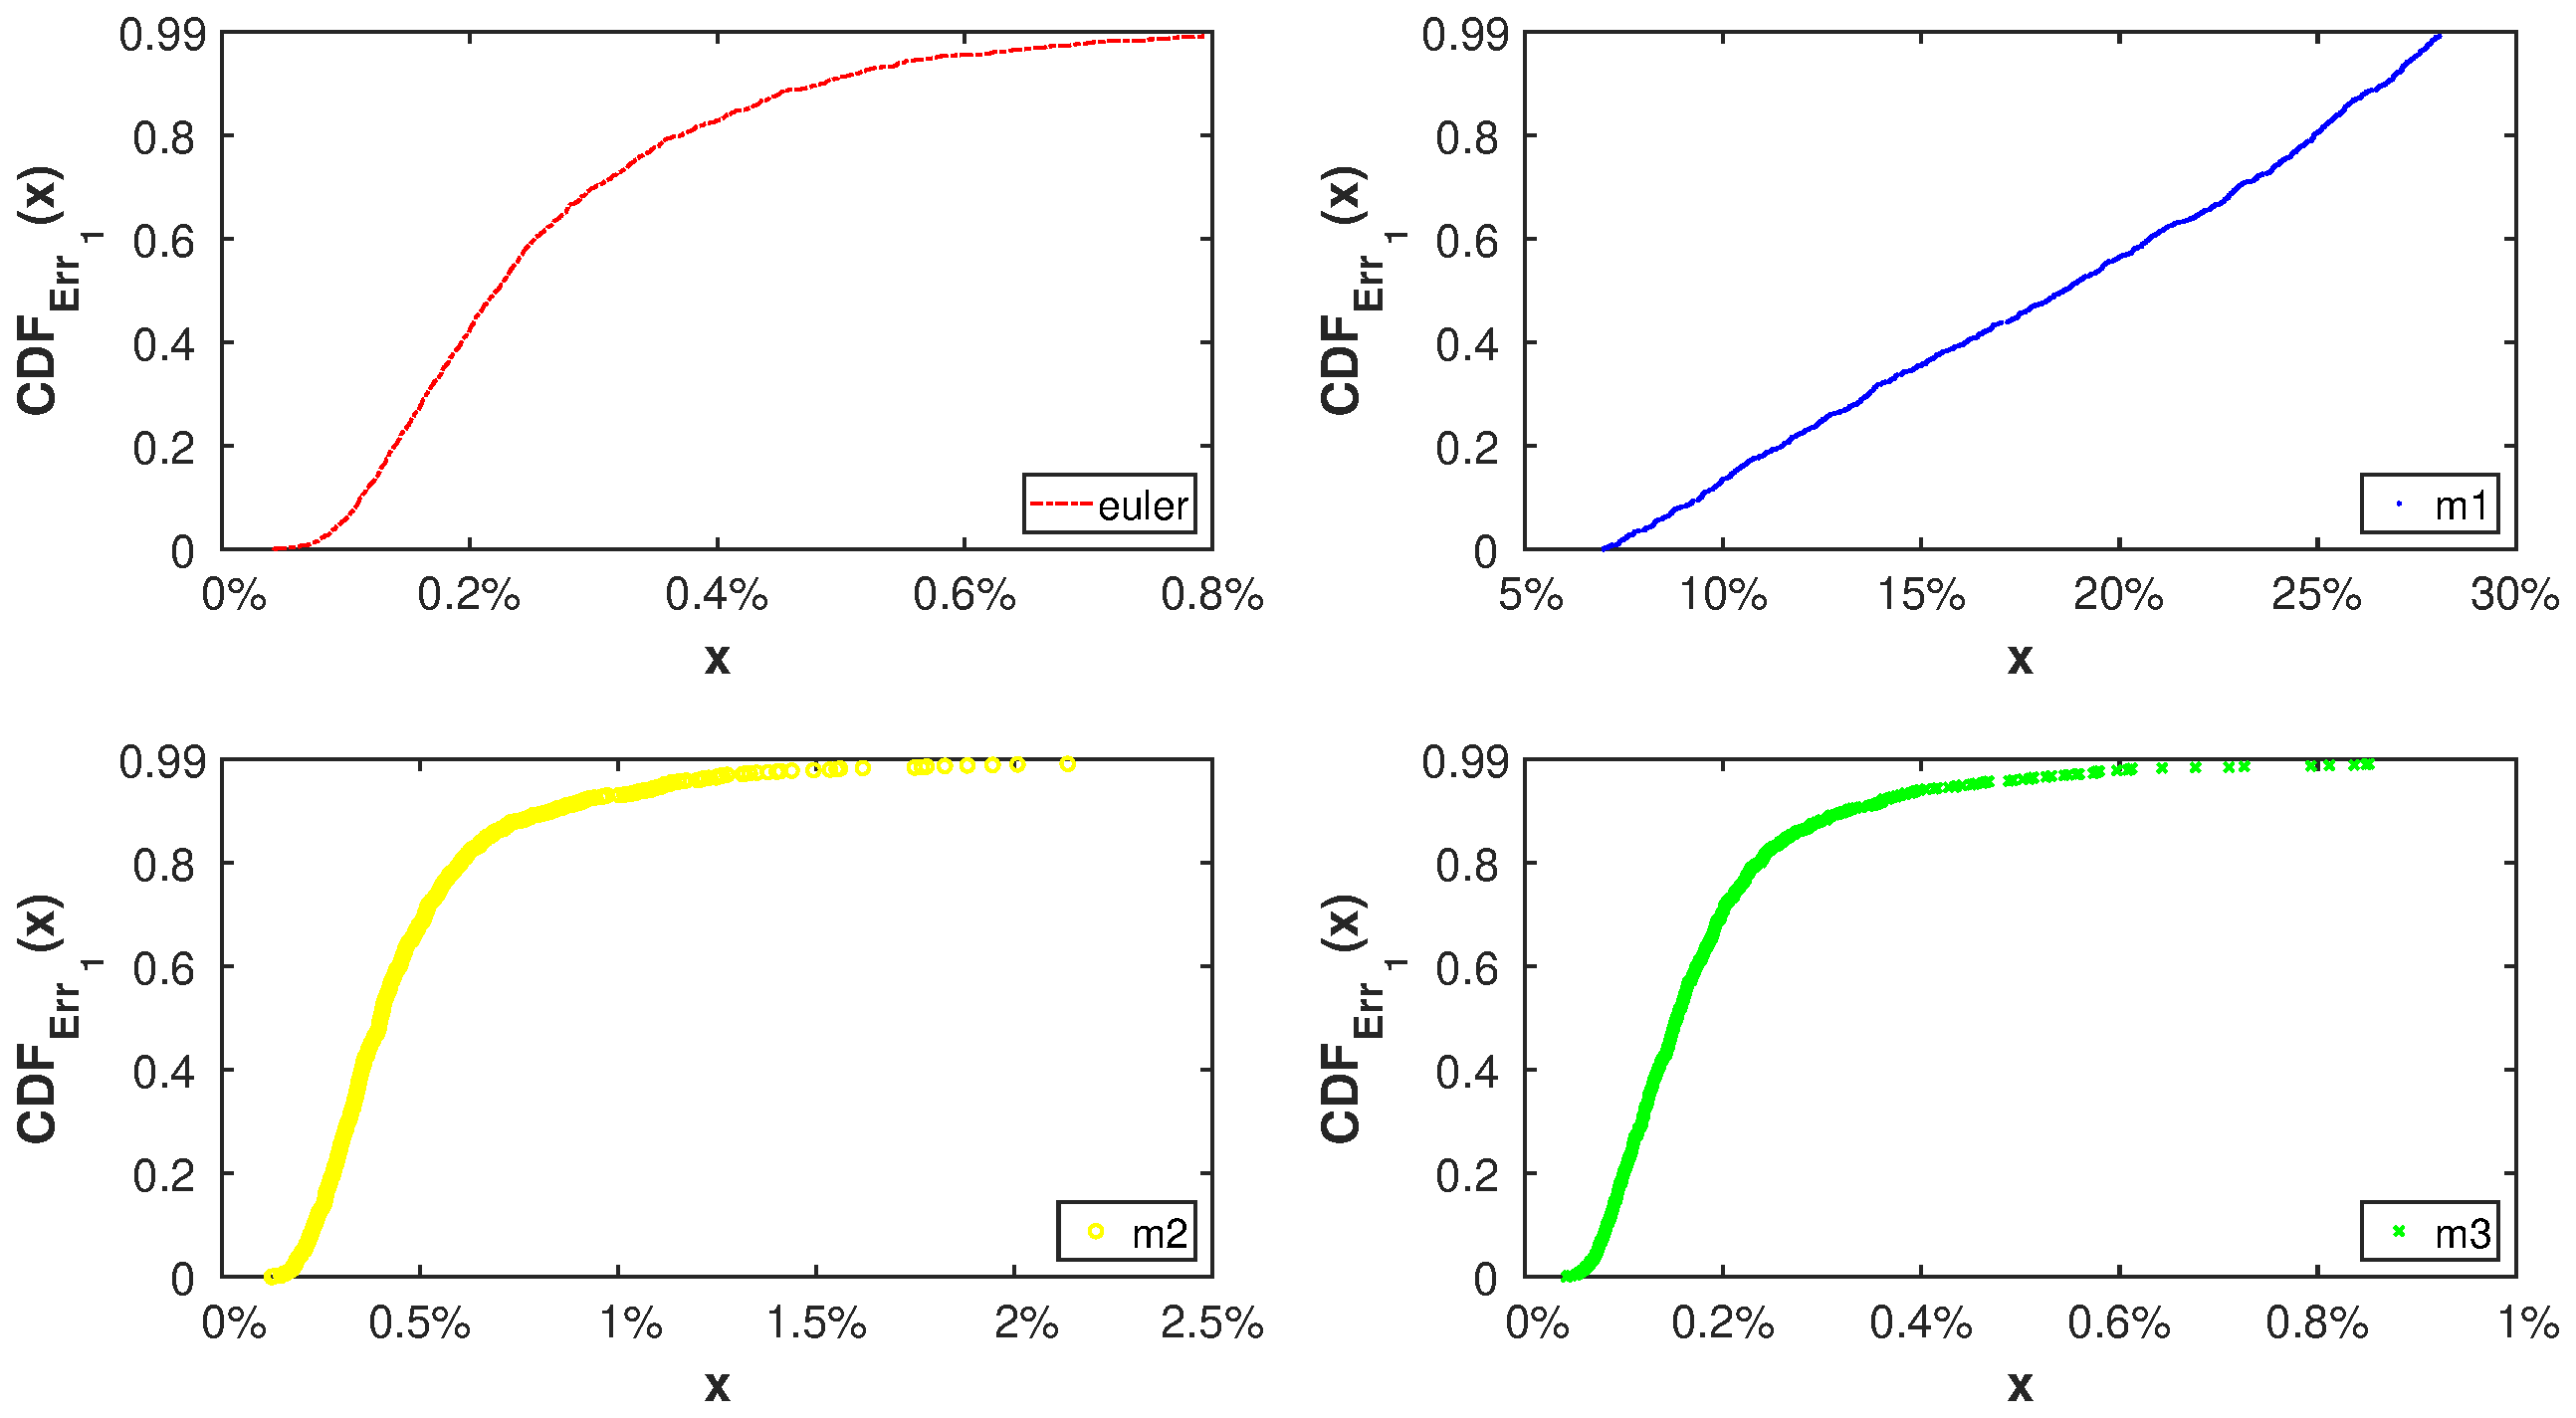
\includegraphics[width=.95\columnwidth]{C:/Users/kevin/Documents/MATLAB/PhD/Magnus/Final/Correction/B0_var/Pdf/temp/error_plot_5.eps}
\end{landscape}
\begin{landscape}
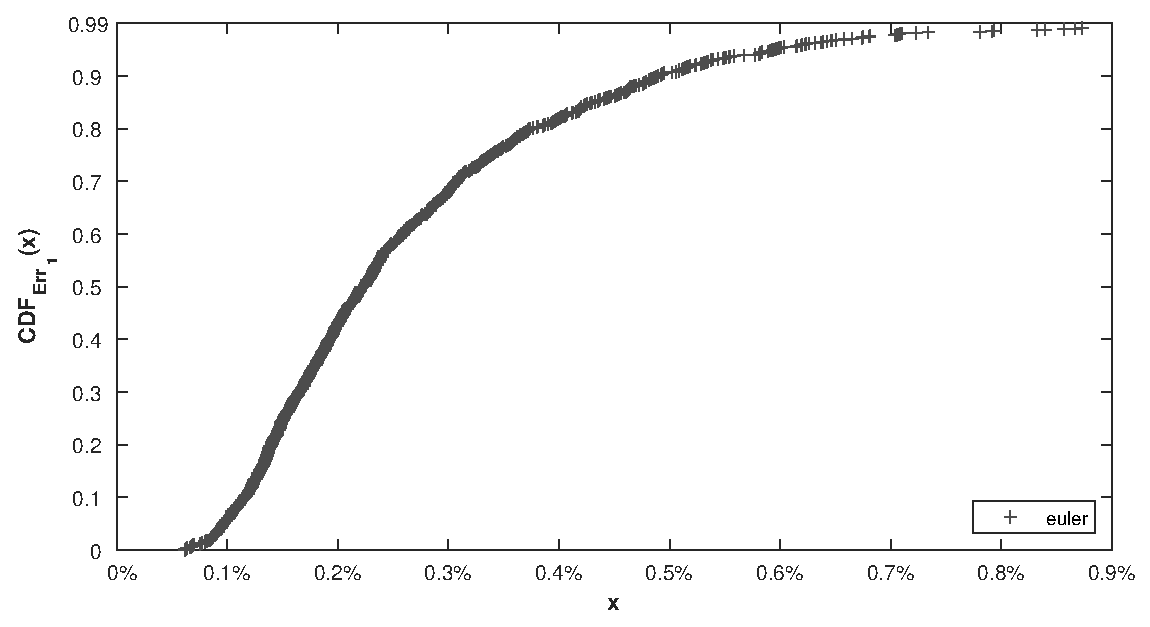
\includegraphics[width=.95\columnwidth]{C:/Users/kevin/Documents/MATLAB/PhD/Magnus/Final/Correction/B0_var/Pdf/temp/error_plot_6.eps}
\end{landscape}
\begin{landscape}
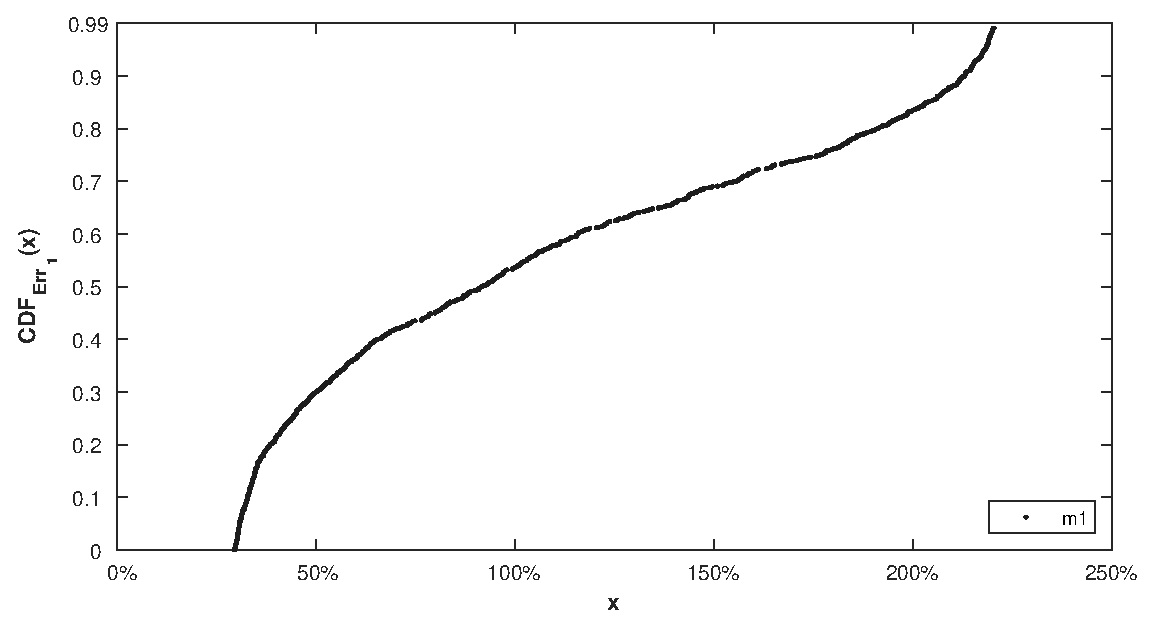
\includegraphics[width=.95\columnwidth]{C:/Users/kevin/Documents/MATLAB/PhD/Magnus/Final/Correction/B0_var/Pdf/temp/error_plot_7.eps}
\end{landscape}
\begin{landscape}
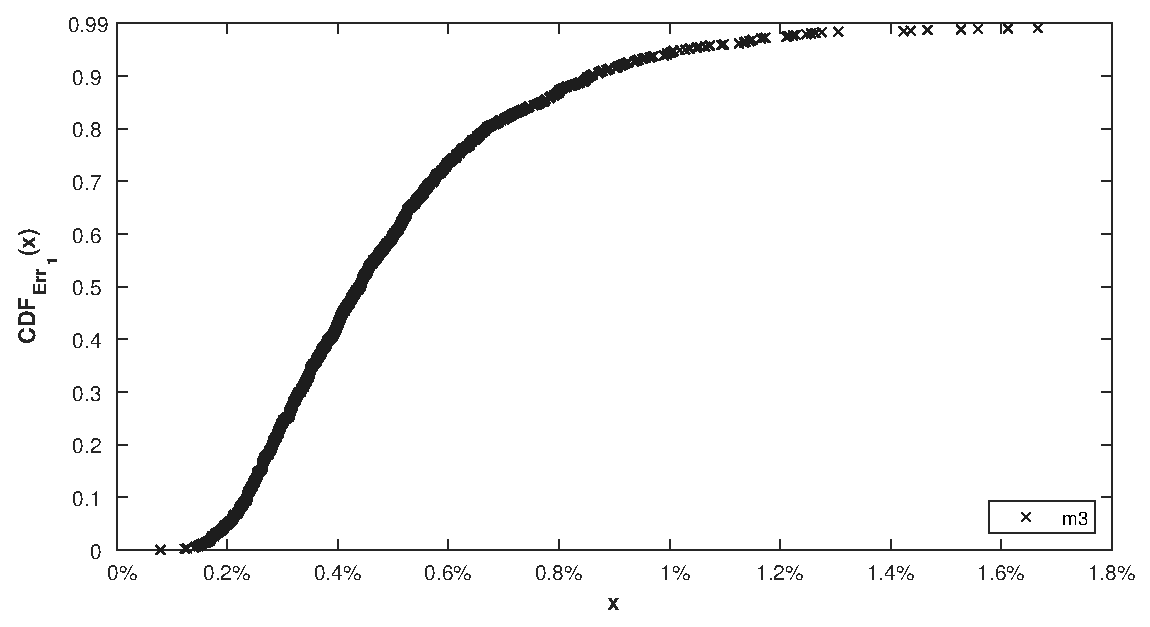
\includegraphics[width=.95\columnwidth]{C:/Users/kevin/Documents/MATLAB/PhD/Magnus/Final/Correction/B0_var/Pdf/temp/error_plot_8.eps}
\end{landscape}
\begin{landscape}
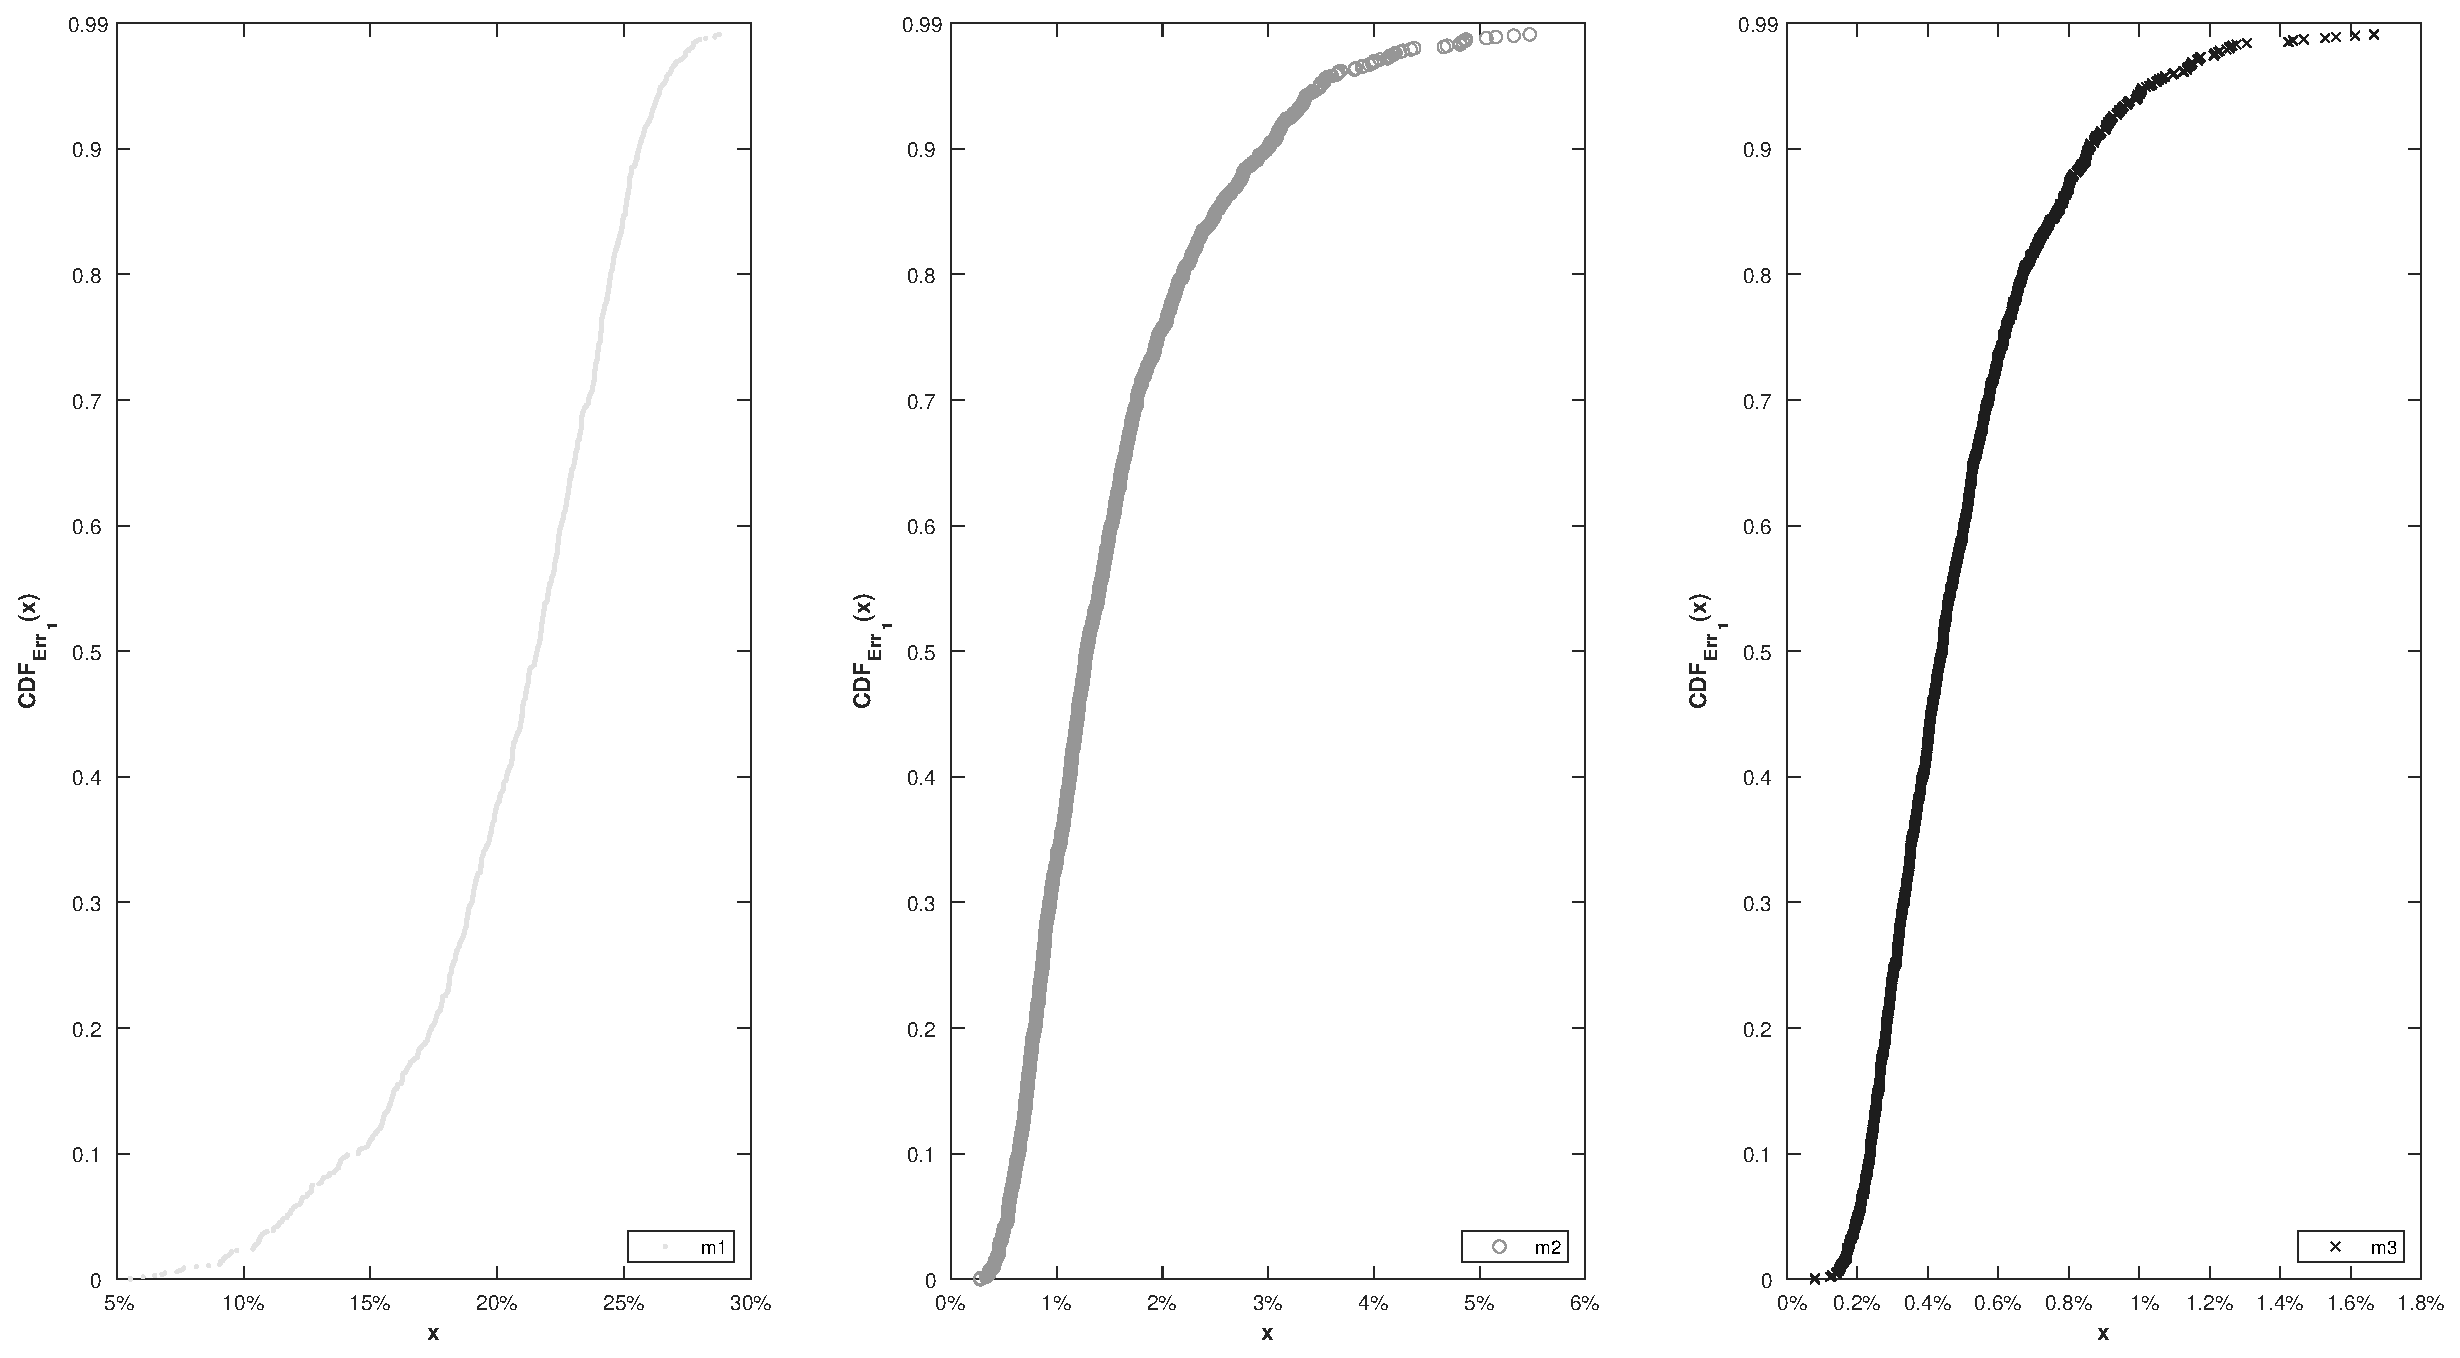
\includegraphics[width=.95\columnwidth]{C:/Users/kevin/Documents/MATLAB/PhD/Magnus/Final/Correction/B0_var/Pdf/temp/error_plot_9.eps}
\end{landscape}
\begin{landscape}
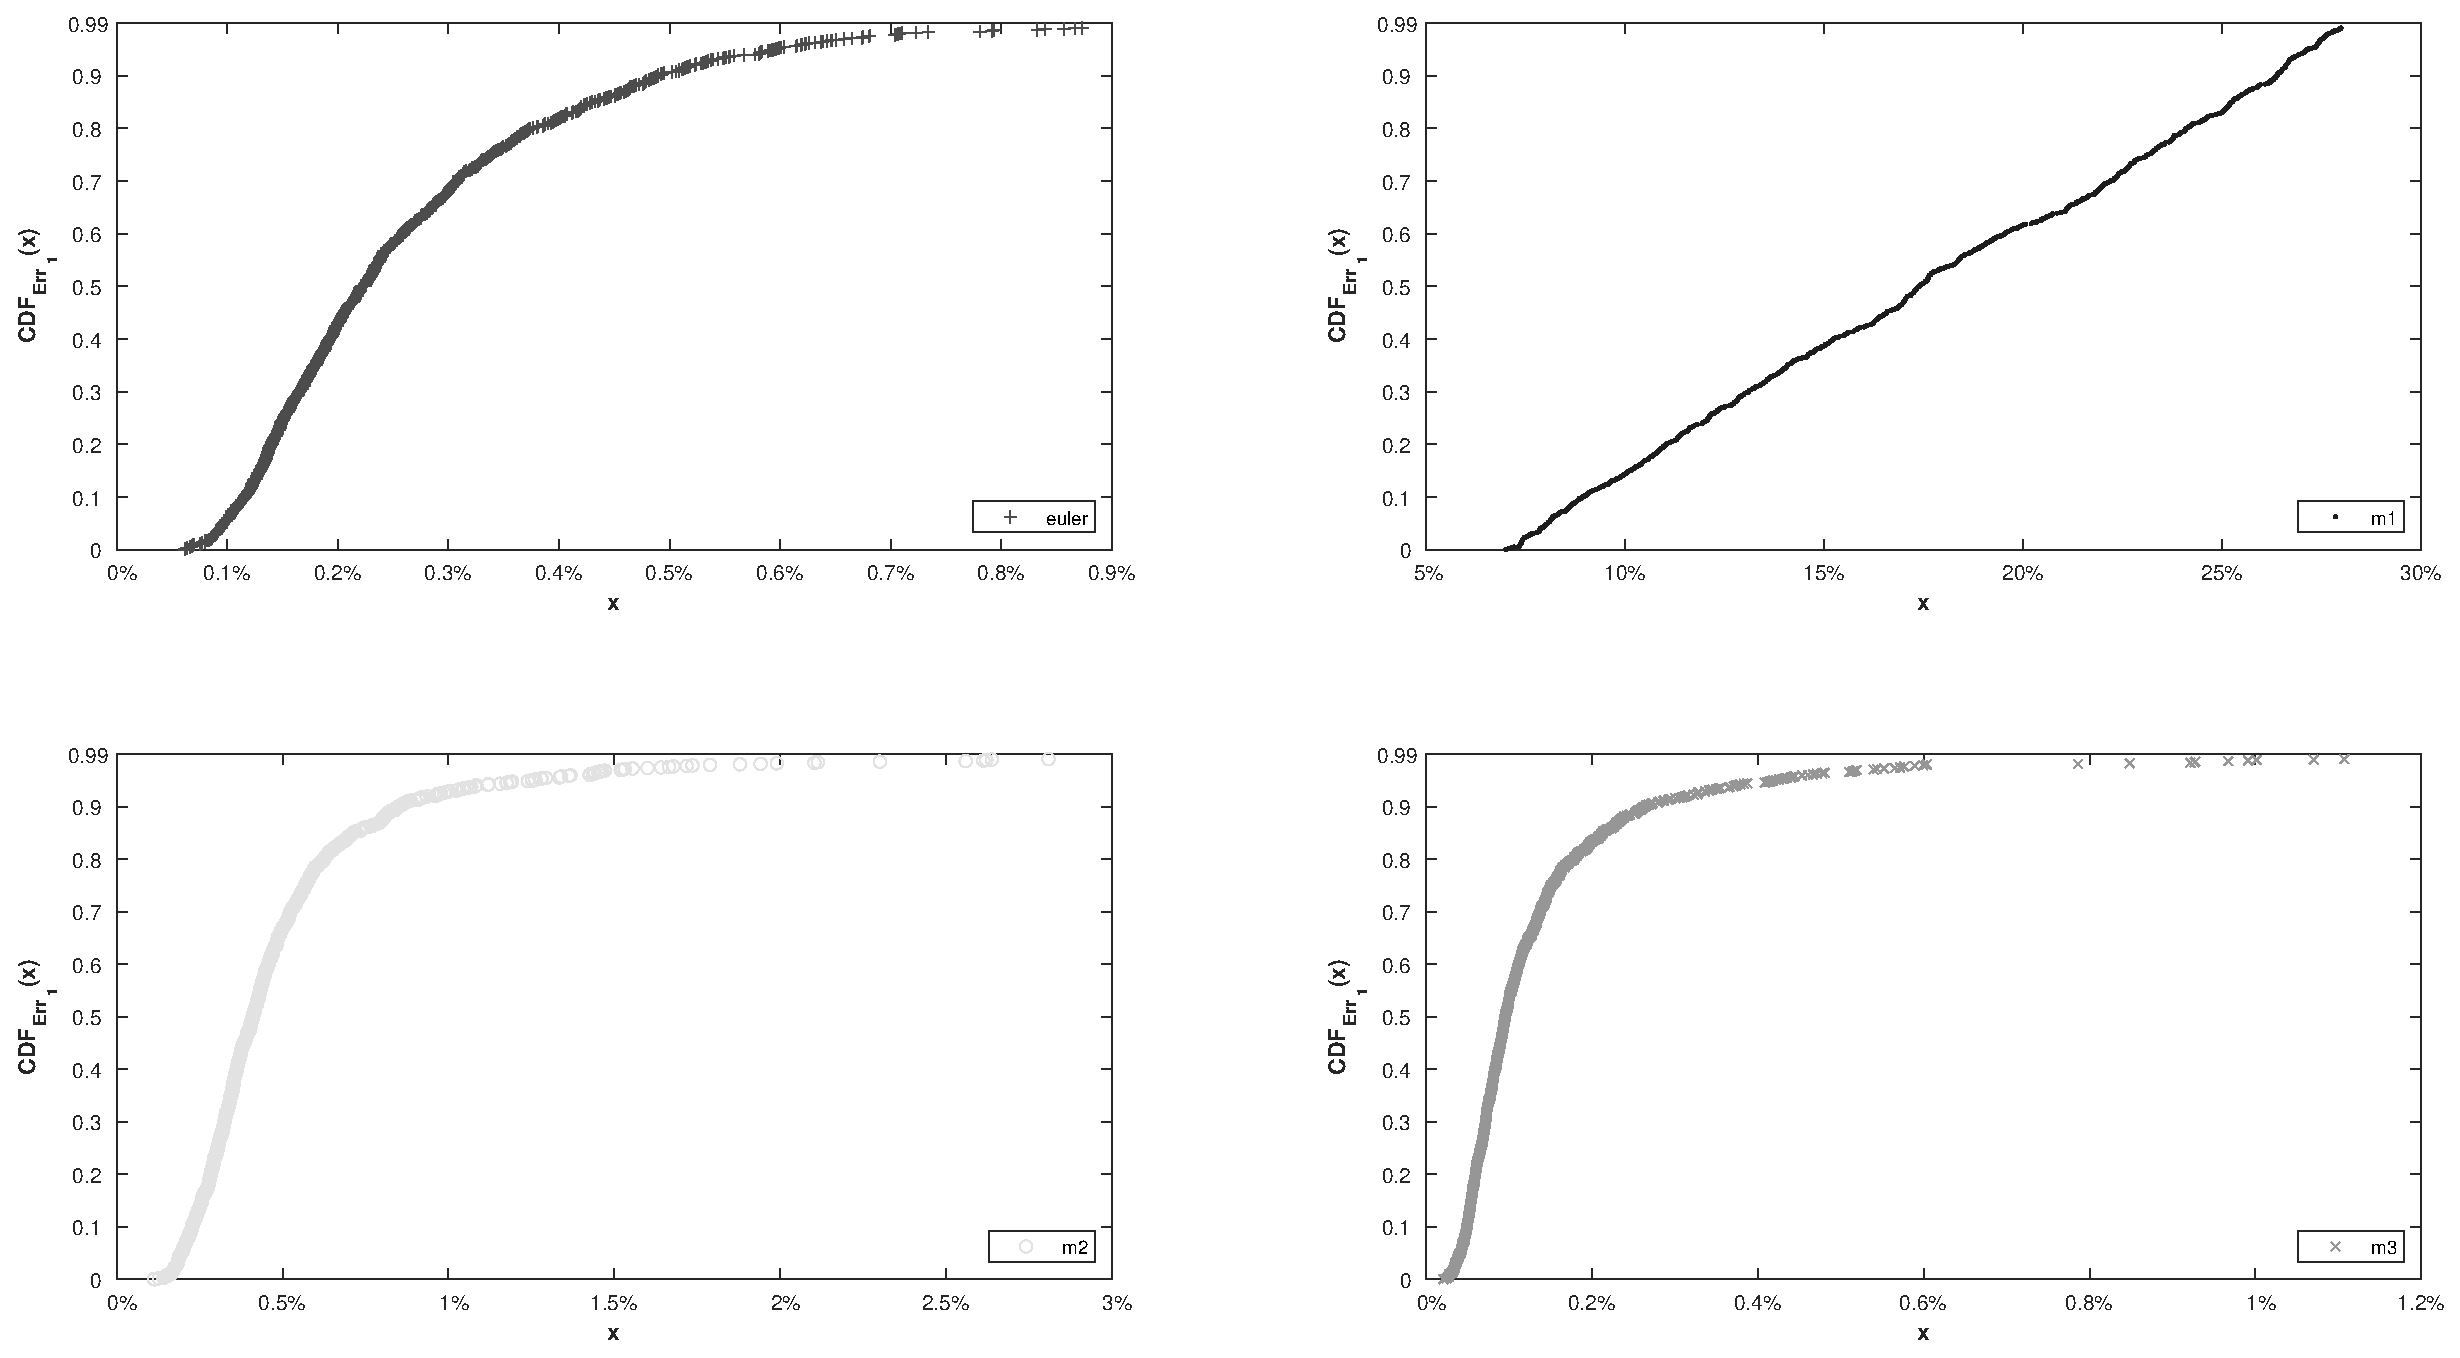
\includegraphics[width=.95\columnwidth]{C:/Users/kevin/Documents/MATLAB/PhD/Magnus/Final/Correction/B0_var/Pdf/temp/error_plot_10.eps}
\end{landscape}


%\subsubsection*{Parameters}
	%%\begin{table}%
		%\begin{tabular}{@{}*{2}{c}@{}}
\text{\textbf{Parameter}} & \text{\textbf{value}}\\
\toprule\\
$t_0$ & $0$\\
$T$ & $1$\\
\verb+N_fine+ & $10000$\\
$N$ & $1000$\\
\verb+M_fine+ & $1000$\\
$M$ & $1000$\\
$d$ & $2$\\
\end{tabular}

		%%\caption{}
		%%\label{}
	%%\end{table}
%\subsubsection*{Errors}
	%%\begin{table}%
		%\begin{compactenum}
\item Errors for $X(1,1,:,:)$:
\begin{compactenum}
\item Reference method: exact\\
\begin{tabular}{@{}*{5}{c}@{}}
\text{\textbf{Error}} &\text{\textbf{euler}} &\text{\textbf{m1}} &\text{\textbf{m2}} &\text{\textbf{m3}} \\
\toprule\\
(abs error) L2 &$0.00612649$ &$0.431044$ &$0.000170138$ &$0.000170138$ \\
(rel error) min &$0$ &$0$ &$0$ &$0$ \\
(rel error) max &$0.00519639$ &$0.576061$ &$9.72097e-05$ &$9.72097e-05$ \\
(rel error) mean &$0.00373177$ &$0.279633$ &$4.52479e-05$ &$4.52479e-05$ \\
\end{tabular}
\end{compactenum}
\item Errors for $X(1,2,:,:)$:
\begin{compactenum}
\item Reference method: exact\\
\begin{tabular}{@{}*{5}{c}@{}}
\text{\textbf{Error}} &\text{\textbf{euler}} &\text{\textbf{m1}} &\text{\textbf{m2}} &\text{\textbf{m3}} \\
\toprule\\
(abs error) L2 &$0.00213927$ &$0.0771372$ &$0.0217018$ &$0.0084237$ \\
(rel error) min &$0.000120492$ &$0.0197843$ &$0.0056921$ &$0.00628867$ \\
(rel error) max &$0.0140499$ &$0.433351$ &$0.138571$ &$0.0323207$ \\
(rel error) mean &$0.00771088$ &$0.239473$ &$0.065535$ &$0.0158499$ \\
\end{tabular}
\end{compactenum}
\item Errors for $X(2,2,:,:)$:
\begin{compactenum}
\item Reference method: exact\\
\begin{tabular}{@{}*{5}{c}@{}}
\text{\textbf{Error}} &\text{\textbf{euler}} &\text{\textbf{m1}} &\text{\textbf{m2}} &\text{\textbf{m3}} \\
\toprule\\
(abs error) L2 &$0.00131998$ &$0.0788425$ &$5.32062e-05$ &$5.32062e-05$ \\
(rel error) min &$0$ &$0$ &$0$ &$0$ \\
(rel error) max &$0.0013011$ &$0.120453$ &$4.61903e-05$ &$4.61903e-05$ \\
(rel error) mean &$0.000933184$ &$0.0618502$ &$2.20918e-05$ &$2.20918e-05$ \\
\end{tabular}
\end{compactenum}
\item Total Errors:
\begin{compactenum}
\item Reference method: exact\\
\begin{tabular}{@{}*{2}{c}@{}}
\text{\textbf{Method}} & \text{$\mathbb{E}[Err_{ 1}]$}\\
\toprule
euler &$0.27\,\%$ \\
m1 &$17.6\,\%$ \\
m2 &$0.523\,\%$ \\
m3 &$0.147\,\%$ \\
\end{tabular}
\end{compactenum}
\end{compactenum}

		%%\caption{}
		%%\label{}
	%%\end{table}
%\subsubsection*{Computational times}
	%%\begin{table}%
		%\begin{tabular}{@{}*{4}{c}@{}}
\text{\textbf{Method}} &\text{\textbf{Log}} &\text{\textbf{Matrix Exp}} &\text{\textbf{Total}}\\
\toprule\\
\text{euler} & 0 & 0 & 20.4149 \\
\text{m1} & 0.0135129 & 1.68122 & 1.69474 \\
\text{m2} & 0.0248556 & 1.65356 & 1.67842 \\
\text{m3} & 0.0422674 & 1.63387 & 1.67613 \\
\end{tabular}

		%%\caption{}
		%%\label{}
	%%\end{table}
%\subsubsection*{Figures}
		%\input{Pdf/temp/figures.tex}
%%\begin{landscape}
	%%%\begin{figure}%
	%%\includegraphics[width=.95\columnwidth]{Pdf/temp/figures.png}%
	%%%\caption{}%
	%%%\label{}%
	%%%\end{figure}
%%\end{landscape}
\end{document}